
\documentclass{article}
\usepackage{float}
\usepackage{array,multirow,graphicx}
\usepackage{subfig}
\usepackage{lipsum}
\usepackage{tikz}
\usepackage{eso-pic}
\usepackage{changepage}
\usepackage{afterpage}
\usepackage[document]{ragged2e}
\usepackage[none]{hyphenat}
\usepackage[margin=1in,footskip=0.25in]{geometry}
\usepackage{array}
\usepackage{siunitx}
\usepackage{color,soul}
\usepackage{placeins}
\usepackage{siunitx}
\usepackage{microtype}
\usepackage[backend=biber]{biblatex}
\usepackage{hyperref}
\usepackage[toc,page]{appendix}
\usepackage[toc]{glossaries}
\usepackage[subfigure]{tocloft}
\usepackage{rotating}
\usepackage[printwatermark]{xwatermark}
\usepackage{xcolor}
\usepackage{changepage}
% \usepackage{tgbonum}
% \usepackage[utf8]{inputenc}

\hypersetup{
    colorlinks,
    linkcolor={black!50!black},
    citecolor={blue!50!black},
    urlcolor={blue!80!black}
}

\cftsetindents{subsection}{.25in}{.4in}

\usepackage[flushleft]{threeparttable}
\newcolumntype{C}[1]{>{\centering\let\newline\\\arraybackslash\hspace{0pt}}m{#1}}

\definecolor{ULred}{HTML}{B10820}

\usepackage{chngcntr}
\counterwithin{table}{section}
\counterwithin{figure}{section}

\setlength{\parskip}{1em}

\addbibresource{PPVReport.bib}
\pdfoptionpdfminorversion=6

\loadglsentries{glossary.tex}

\makeglossaries

\newcommand{\adjustimg}{% Horizontal adjustment of image
  \checkoddpage%
  \ifoddpage\hspace*{\dimexpr\evensidemargin-\oddsidemargin}\else\hspace*{-\dimexpr\evensidemargin-\oddsidemargin}\fi%
}
\newcommand{\centerimg}[2][width=\textwidth]{% Center an image
  \makebox[\textwidth]{\adjustimg\includegraphics[#1]{#2}}%
}

% \newenvironment{Arialfont}{\fontfamily{<familyname>}\selectfont}{\par}

% \newsavebox\mybox
% \savebox\mybox{\tikz[color=gray,opacity=0.5]\node{DRAFT};}
% \newwatermark*[
% allpages,
% angle=65,
% scale=15,
% xpos=-65,
% ypos=20
% ]{\usebox\mybox}

\begin{document}
\thispagestyle{empty}
\vspace*{-1.25in}
\hspace*{-1.05in}
\makebox[0pt][l]{%
  \raisebox{-\totalheight}[0pt][0pt]{%
    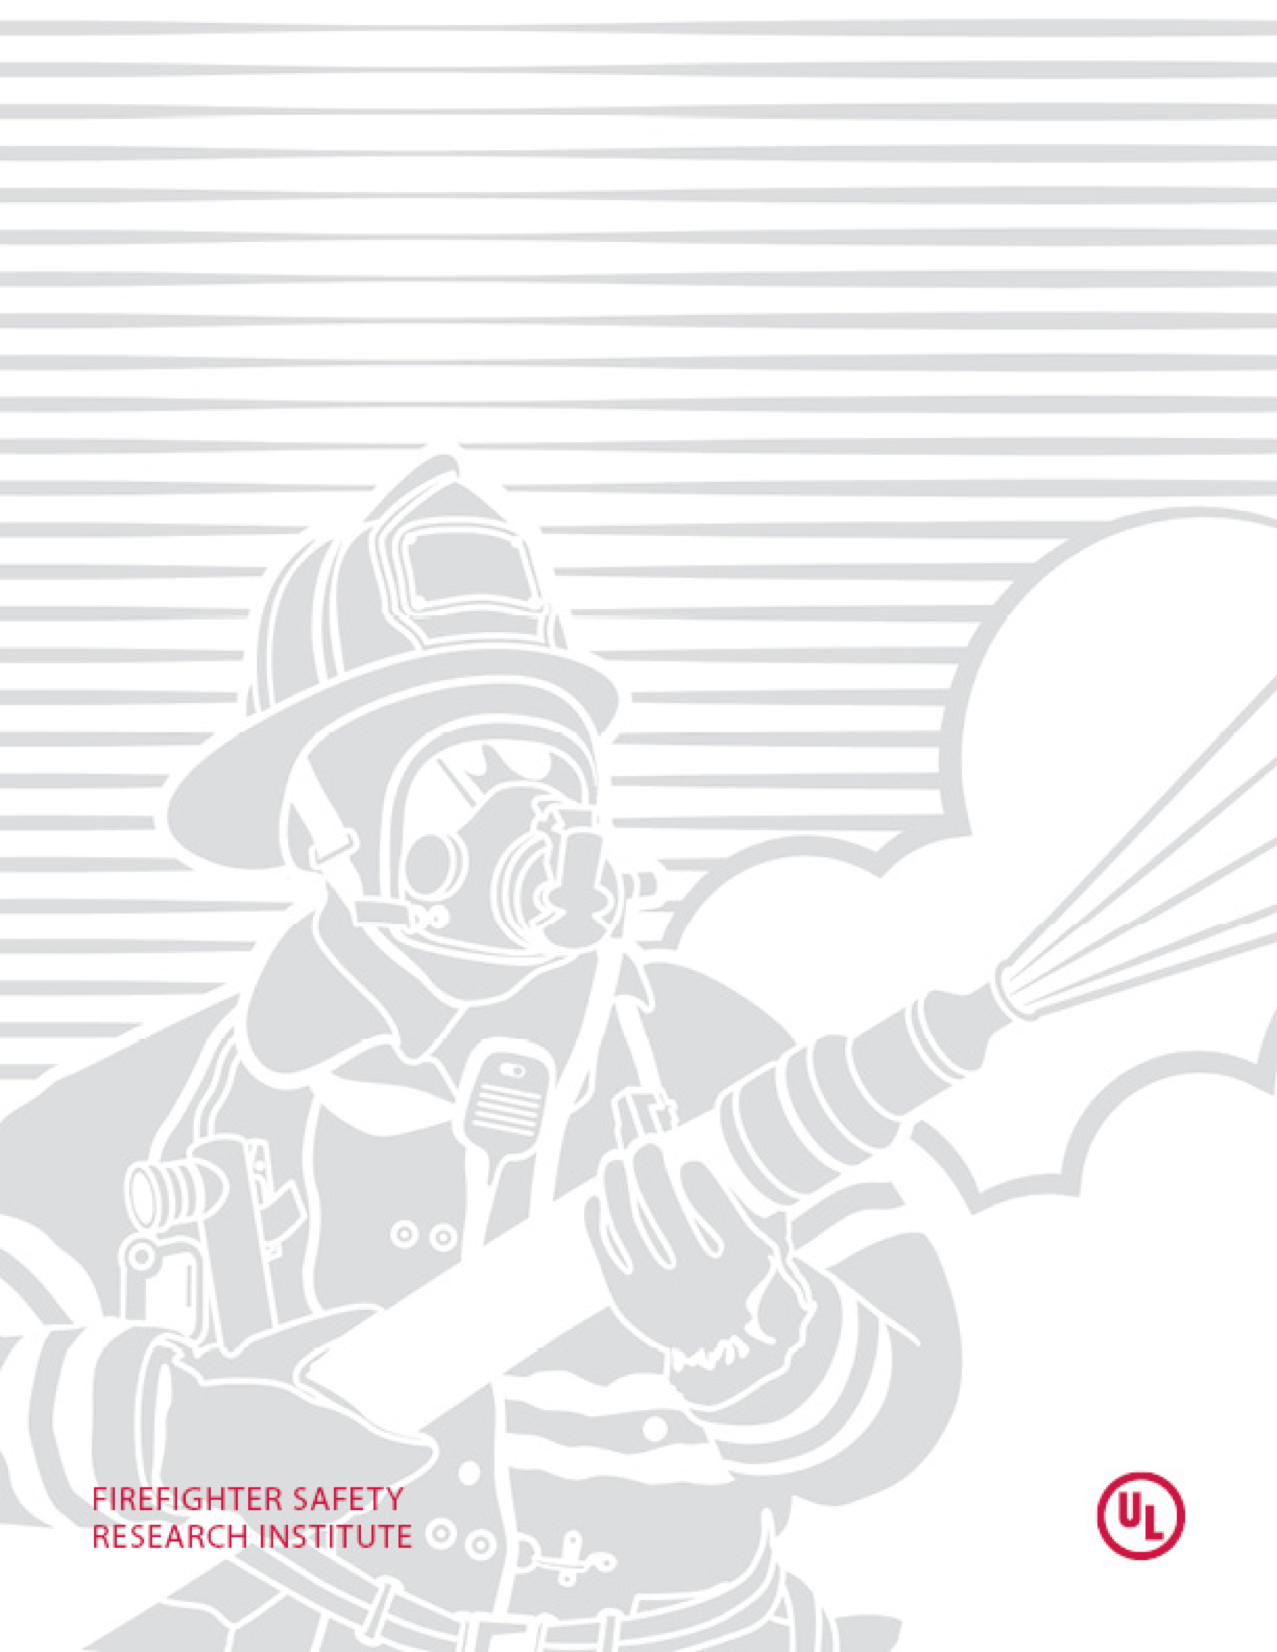
\includegraphics[width=\paperwidth,height=\paperheight]{0_Images/FD_Summary_Cover_Image.png}}}%

\color{ULred}

\begin{adjustwidth}{-.25in}{-.25in}
\fontsize{30}{40}\selectfont {\fontfamily{qhv}\selectfont Fire Service Summary Report:} \\
\vspace*{.1in}
\huge
{\fontfamily{qhv}\selectfont Study of the Effectiveness of Fire Service Positive \\ Pressure Ventilation During Fire Attack in Single \\ Family Homes Incorporating Modern Construction \\Practices} \\
\normalsize
\vspace*{.5in}
\fontfamily{qhv}\selectfont\today
\end{adjustwidth}

\clearpage

\vspace*{-1.75in}
\hspace*{-1.075in}
\makebox[0pt][l]{%
  \raisebox{-\totalheight}[0pt][0pt]{%
    
\includegraphics[scale=1.05]{0_Images/FD_Summary_2nd_Page.png}}}%

\normalsize
\color{black}
\clearpage

\begin{center}
DISCLAIMER\\
\end{center}

\vspace*{\baselineskip}

In no event shall UL be responsible to anyone for whatever use or nonuse is made of the information contained in this Report and in no event shall UL, its employees, or its agents incur any obligation or liability for damages including, but not limited to, consequential damage arising out of or in connection  with the use or inability to use the information contained in this Report. Information conveyed by this Report applies only to the specimens actually involved in these tests. UL has not established a factory Follow-Up Service Program to determine the conformance of subsequently produced material, nor has any provision been made to apply any registered mark of UL to such material. The issuance of this Report in no way implies Listing, Classification or Recognition by UL and does not authorize the use of UL Listing, Classification or Recognition Marks or other reference to UL on or in connection with the product or system.

\begin{center}
FORWARD
\end{center}

\vspace*{\baselineskip}

This document is a subset of the full technical report titled, “Study of the Effectiveness of Fire Service Positive Pressure Ventilation During Fire Attack in Single Family Homes Incorporating Modern Construction Practices,” that can be downloaded at \href{www.ULfirefightersafety.com}{www.ULfirefightersafety.com}. There is no additional information provided in this document rather it includes introductory material, a summary of the experimental setup, fire service tactical considerations and summary of the full report.  Please refer to the full report for more detail and discussion of the results.

\clearpage

\section{Introduction}
The purpose of this study is to increase firefighter safety by providing the fire service with credible scientific information, developed from full-scale fire testing in representative modern single family homes, on the usage of positive pressure ventilation fans during fire attack. 

\subsection{Background}
NFPA estimates \cite{NFPAFireLoss} that from 2002-2011, U.S. fire departments responded to an average of 398,000 residential fires annually. These fires caused an estimated annual average of 2,820 civilian deaths and 13,780 civilian injuries. More than 70\% of the reported home fires and 84\% of the fatal home fire injuries occurred in one- or two- family dwellings, with the remainder in apartments or similar properties. For the 2006-2009 period, there were an estimated annual average 35,743 firefighter fire ground injuries in the U.S. \cite{NFPAFFInjuries} The rate of traumatic firefighter deaths occurring outside structures or from cardiac arrest has declined, while at the same time, firefighter deaths occurring inside structures has continued to climb over the past 30 years. \cite{NFPALast30} Ventilation is believed to be a significant contributing factor to this continued climb in firefighter injuries and deaths. Developing the proper knowledge about the use of PPV will enable more departments to implement its use with the confidence of knowing when to apply it to increase the safety of their members, whether in place of or supplementing current ventilation tactics.

Over the last 5 years of fire service research, it has become clear that the fire service needs more information and knowledge about fire dynamics and how the changing fire environment impacts their tactics and safety. Studying the modern fire environment has shown that fires grow faster today than ever before, they become ventilation limited (or run out of air) and the control of that air during fire attack is critical to a safely mitigated fire incident \cite{ChangingResdFires_Kerber}. Two previous UL studies have examined horizontal ventilation \cite{One_Two_Family_Fires_Kerber} and vertical ventilation \cite{UL_VerticalVent} which are the two most common types of ventilation used by the fire service on a daily basis. The results of these studies have been disseminated to the fire service with positive feedback \cite{HowToKeepFirefighterSafer_Goldfeder}, \cite{SurbarbanFirefighting_Knapp} regarding the integration of tactical considerations into their standard operating procedures. The fire service anticipates increased safety due to the knowledge obtained from UL’s research as they better understand the necessary coordination of ventilation and suppression. Following each presentation on the horizontal and vertical ventilation results, firefighters have also consistently sought similar data and knowledge for the use of positive pressure ventilation (PPV). 

PPV is a technique used by the fire service to remove smoke, heat and other combustion products from a structure. This technique uses a fan or multiple fans to create a higher pressure inside the home in order to speed up the flow to the lower pressure outside of the house (Figure \ref{fig:PPV_Diagram}). This allows the fire service to perform tasks within the structure in a more tenable atmosphere. Since it was introduced in the 1980’s, PPV has become an important tool in the fire service. Many departments have adopted this technique after water has been applied to the fire to assist in the overhaul phase of the fire. Several other departments have incorporated it as part of their initial fire attack. When used during fire attack, a PPV fan or blower is placed at the entry point of the attack crew and air is forced through the home and out through an exhaust point ahead of the crew. Under ideal conditions, visibility is increased as smoke and heat are forced ahead of the attack crew and away from occupants inside. This makes the fire attack, search, and other fire ground operations easier and safer to complete.


\begin{figure}[H]
	\centering
	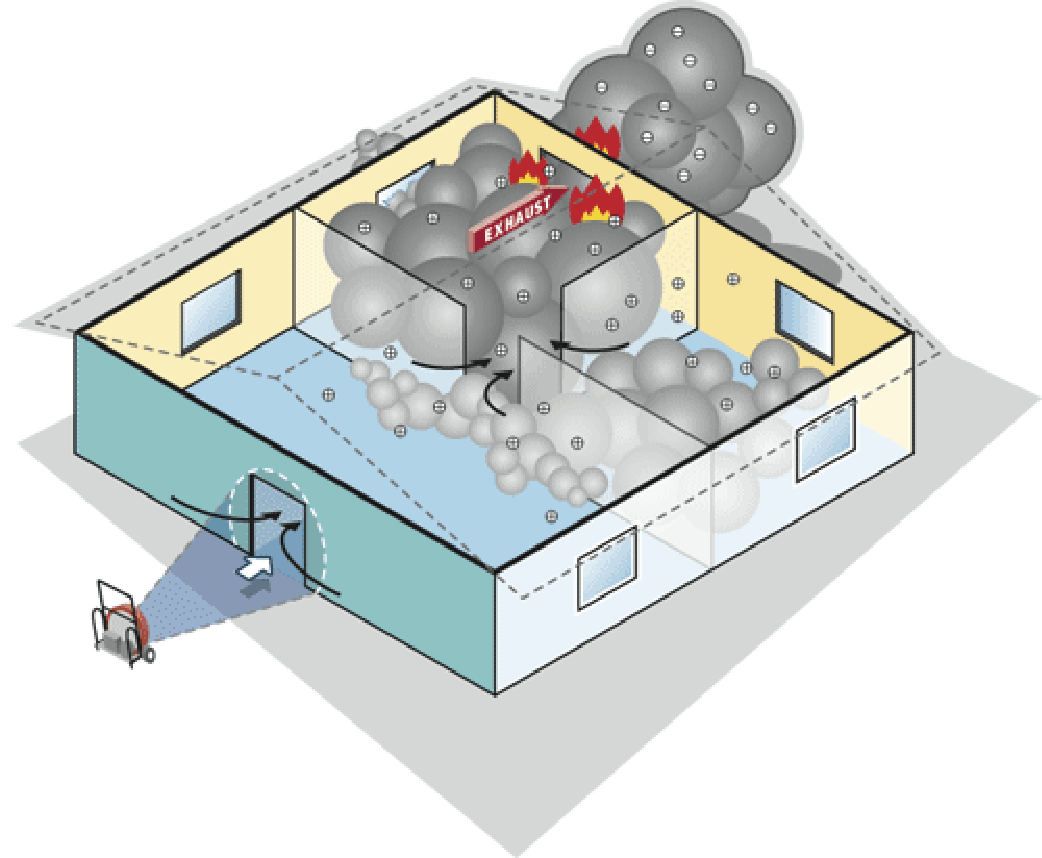
\includegraphics[width = 4in]{0_Images/Tactical_Considerations/Exhaust_Over_Cone/ppv_illistration.pdf}
	\caption{Diagram showing the basic application of positive pressure ventilation}
	\label{fig:PPV_Diagram}
\end{figure}

Since its inception, PPV has become an important tool in the fire service, yet its use has been polarizing. Some departments have developed confidence in using PPV, citing its positive impact on firefighter safety. A majority of departments refuse to use PPV because of the uncertainty created by the unanswered questions or a negative experience with the technology. Constrained by current economic conditions, many departments have limited staffing or have had their staffing reduced and are experimenting with ways to utilize technologies such as positive pressure ventilation fans during fire attack. However, risks exist when its use is not accompanied by appropriate scientific investigations or post-release surveillance of the impact on firefighter and occupant safety. There have been incidents where PPV has been incorporated into firefighting tactics without developing a scientific basis of their use. The lack of knowledge has led to improper usage, misapplication, and numerous injuries and line of duty deaths \cite{NIOSHF2000-44} \cite{NIOSH98F-32} \cite{TexasFMFY07-02} \cite{ContraCostaFalaityInvestigation} \cite{NIOSHF2004-02} \cite{NIOSHF2002-12}. These referenced reports detail the circumstances under which firefighters lost their lives and in each of these cases a PPV fan was in operation. In most of the incidents, it is not clear what role the PPV may have played due to the complexity of the incident and many simultaneous actions. 

Some fire departments have utilized PPV fans after water was applied to the fire but prior to fire control. In these situations, it was observed that fire will intensify while a fan is being used as is expected with additional oxygen made available by the fan. Fire service training on the proper use of fans and their impact on fire dynamics has been difficult. Fire service training buildings are not able to safely replicate the ventilation limited fire conditions needed to understand the impact of PPV. That limitation is coupled with the safety requirement to use wood based fuels in training, which does not replicate the speed or magnitude in which a fire grows, spreads, and reacts to the oxygen added by the PPV fan. This same requirement is placed on acquired structure burn training. Even if realistic home geometries become available, the fire service is not able to use realistic fuels such as sofas, per NFPA 1403 (the Standard on Live Fire Training Evolutions). Additionally, there has been at least one training incident (see Figure \ref{fig:PPVTrainingInj}) where an instructor and trainee have been injured from improper use of PPV techniques \cite{LasVegasNews_ChiefsRole}. This underlines the need for developing scientific data that can be used both on the fire scene as well as during firefighter training.

\begin{figure}[H]
	\centering
	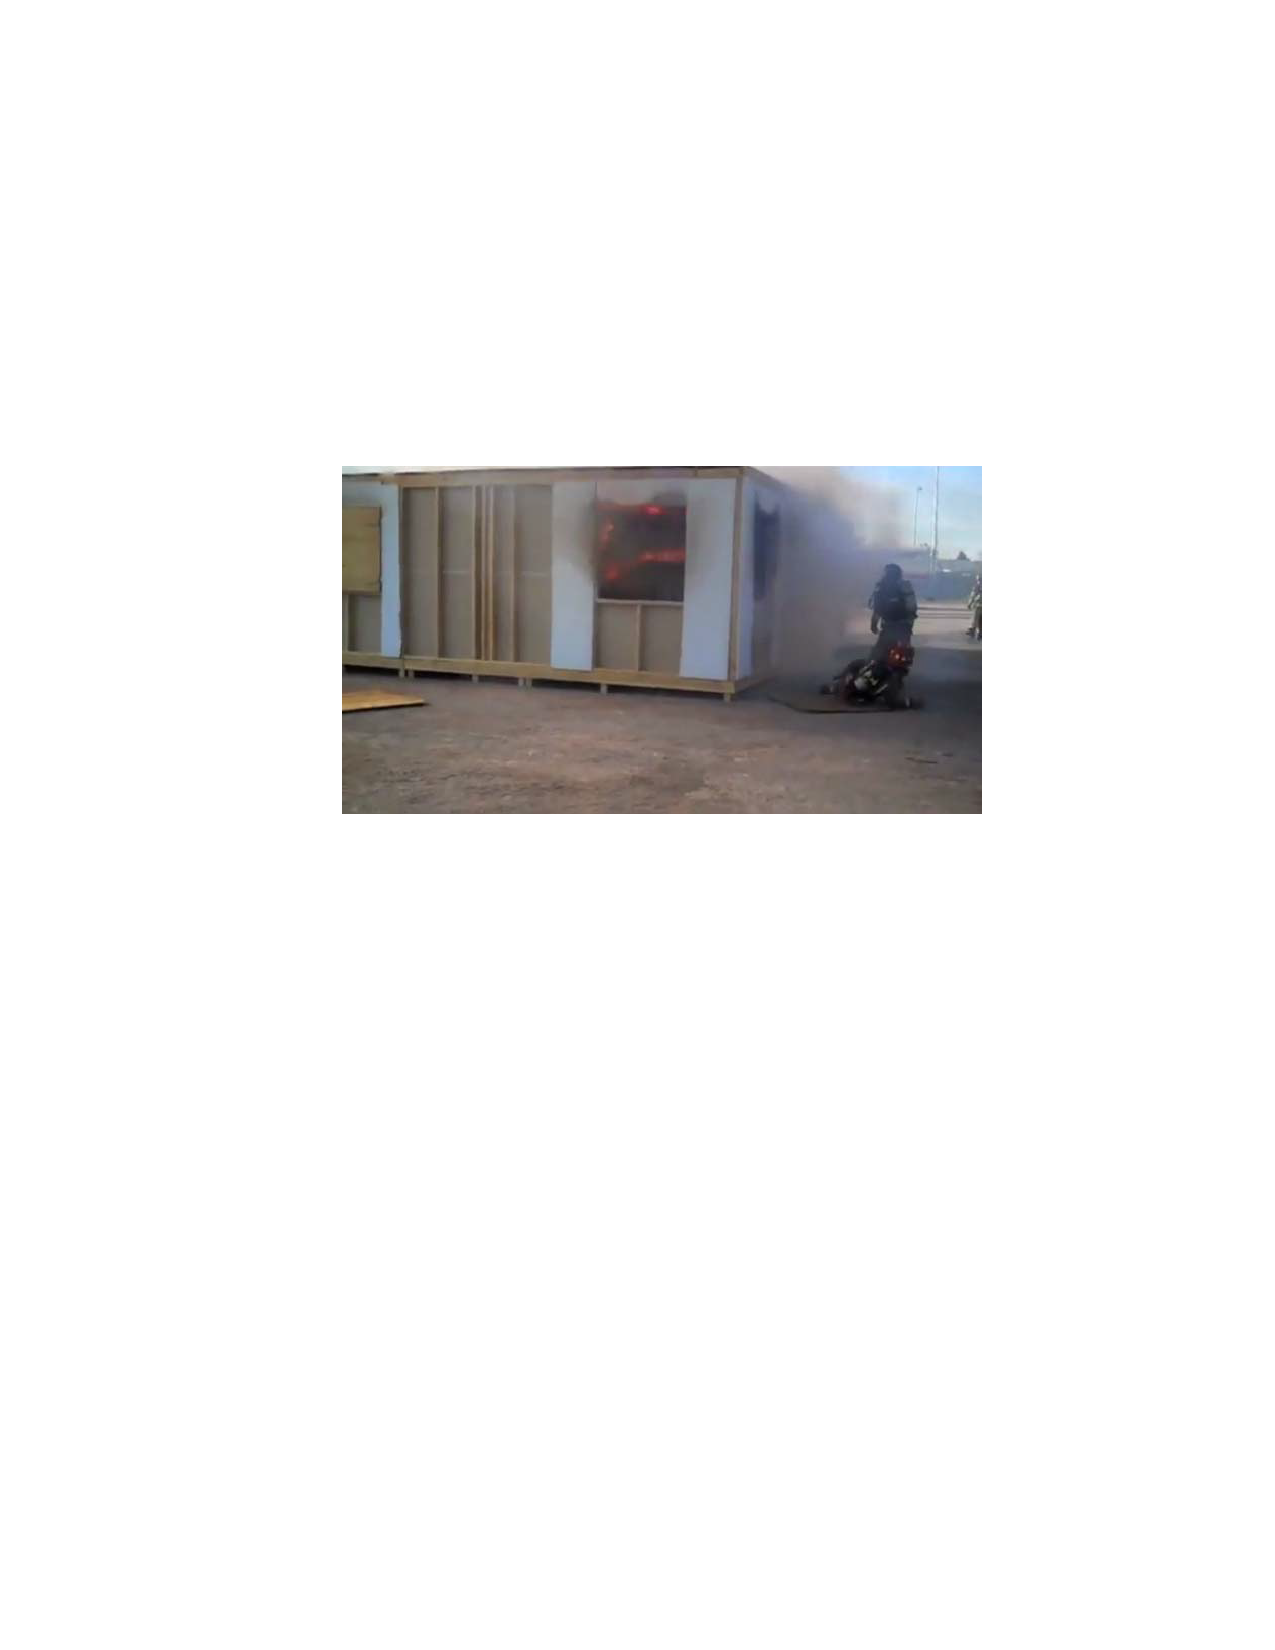
\includegraphics[width = 5in]{0_Images/Background/PPVTrainingInjury.pdf}
	\caption{Moments after lead instructor and student jump out of window to escape further injury during PPV training exercise}
	\label{fig:PPVTrainingInj}
\end{figure}

The use of PPV must be coordinated with fire attack and timed with other ventilation procedures. Traditionally this is done by an interior crew with the fan flow at their back. However, reduced staffing at fire departments have led to firefighters attacking the fire by applying water from outside the structure. A concern with this practice is that applying water externally will “push fire” into the house and subsequently decrease the tenability of occupants inside the structure. Further more, since PPV provides additional oxygen to the fire, used of the tactic can increase the rate of heat released. This can easily exacerbate firefighting operations if the ensuing fire dynamics are not fully understood. Thus, use of PPV needs to be optimized in the overall context of firefighter tactics such as horizontal and vertical ventilation, deployment of firefighter teams, and timing of the use of PPV.

Key factors that need to be addressed to implement PPV safely and most effectively include
the following:

\begin{itemize}
	\item Impact of home structure on PPV effectiveness.
	\begin{itemize}
		\item Home Size
		\item Floor Plan
		\item Void Spaces (e.g attic)
		\item Fuel load
	\end{itemize}
	\item Impact of PPV tactics on fire dynamics.
	\begin{itemize}
		\item Potential of increased hazards associated with forcing fire gases into the eave or attic space.
		\item Potential of blowing fresh air pushing fire through a house or spreading fire from a non-vented room to a vented room.
		\item Impact to occupants (and fire teams) that are in or out of the flow path and may be downstream of the fan.
		\item Conditions created when the flow path to the exhaust is blocked inside the structure.
		\item Transition from a content to a structure fire by forcing hot gases into void spaces.
	\end{itemize}
	\item Integration of PPV with other ventilation techniques
	\begin{itemize}
		\item Comparison to natural horizontal ventilation tactics and development of optimized firefighting ventilation tactics.
		\item Potential hazards associated with commencing PPV while fire attack crews are inside the structure.
	\end{itemize}
	\item Impact of PPV technology and parameters on effectiveness.
	\begin{itemize}
		\item Fan flow rate
		\item Size of exhaust opening and the ideal inlet/exhaust ratio.
		\item Influence the location of exhaust or openings
	\end{itemize}
\end{itemize}

Research organizations and the fire service have made significant contributions to understanding the scope and limitations of the use of the PPV in fire scenarios over the past two decades. However, there are several gaps that limit its use by the fire service. These may be categorized as follows: (i) type of structures used in the research; (ii) fuel loads; (iii) fire ventilation conditions; and (iv) PPV parameters considered. There are further discussed herein. \par

\textbf{Fire Test Structures:} In many studies, fire department training buildings have been used in the experiments. These buildings are typically constructed with metal or concrete walls that absorb energy differently from representative single-family homes \cite{HughesPPVTesting} \cite{KerberPPVinTraining} \cite{SvennsonFireVentilationDuringOperatoins}. 

\textbf{Fuel loads and Fire Ventilation Conditions:} Some of the studies were limited to wood based fuels (e.g., wood pallets, straw). These fuel sources have different burning characteristics than fuel sources (e.g., upholstered furniture, mattress, carpets, stored items, etc.) in representative single family homes in the USA. Thus, findings from these studies \cite{HughesPPVTesting} \cite{KerberPPVinTraining} \cite{SvennsonFireVentilationDuringOperatoins} have limited practical applications for firefighting tactics. \par

In some studies, fuel packages were utilized which do not allow for the realistic ventilation limited fire conditions necessary to make conclusions that are expected in actual incidents \cite{ExekoyePPVHouseFires} \cite{SvenssonFireVentinLargeFireHall} \cite{BowserTacticalVent} \cite{EzekoyePPVStrucuresReport}. These referenced studies utilized stacks of wooden pallets, foam racks with limited amounts of foam, gas burners, or small pans of flammable liquids. These fuel loads are easily repeatable and cost effective, but again limit the practical application of the results. In the absence of ventilation limited conditions, the impact of added oxygen can only improve conditions, which may be misleading to the effects encountered at actual incidents. Some studies have used computational and scale fire modeling due to the high cost of fire testing but have not been validated, and therefore not incorporated into operating procedures \cite{Didona1993modeling} \cite{KerberPPVCFD} \cite{KerberPPVFDS} \cite{TuomisaariVentilationInFirefighting}. \par

\textbf{PPV Parameters:} \mbox{}Additional studies examined the use of PPV fans in large structures and high-rise buildings \cite{SymposiumHighRisePPV} \cite{KerberMadrzyPPVInLargeStructures} \cite{KerberMadrzyPPVInHighRise}. The results of these studies have added to the understanding of the scope and limitations of PPV. However, in most cases, these studies examined the fan's ability to pressurize areas of a building to limit fire and smoke spread, which is very different than blowing air through the fire compartment in one and two family homes. 

Since the initial introduction of fans into the fire service, newer fan technologies have been developed (including conventional, turbo and Pow’Air). These technologies have not yet been investigated in realistic fire scenarios. Also, fan manufacturers have increased flow rates over time. When first introduced, most fans were rated at less than 10,000 cubic feet per minute (CFM); now similar sized fans are rated in excess of 30,000 CFM. The impact of forcing more air into a house fire is not well understood. PPV fans can be found on apparatus around the world and are available in many shapes and sizes. There are portable fans as small as 16 in. and truck mounted fans as large as 60 in. They are powered with gasoline, electric, hydraulic, battery and propane motors. Gasoline powered are the most common, but are accompanied by additional concerns about carbon monoxide (CO) production. Some research has been done on this topic, but CO measurements will be made during these experiments to add to the body of knowledge \cite{KerberMadrzyPPVInLargeStructures}, \cite{LougheedPPVHighRise}. 

This study used representative modern and traditional home geometries, realistic fuel loads representative of furnishings found in today’s homes, fan technologies, sizes and ratings available to the fire service today and simulated response and operational times in order to adequately address the questions and concerns the firefighter community has expressed. In addition it is intended to provide a baseline for choosing when and when not to employ PPA or PPV on the fireground. The results and conclusions of this study are intended to be used to improve firefighting tactics, fire ground safety and fire dynamics knowledge.

\subsection{Limitation and Scope}

The purpose of this study is not to establish if positive pressure attack or positive pressure ventilation are more effective than other types of ventilation. The purpose is to increase the fire service’s knowledge of the impact of these tactics under specific conditions. Since all fireground circumstances cannot be analyzed, it is anticipated that the data developed and this analysis will enable firefighters to complement their previous observations and experiences.

Every fire event that the fire service responds to is unique. The range of fire ground variables at each fire event make firefighting complex. In this investigation, key variables were identified and bounded to develop the data under controlled conditions. These variables included:

\begin{itemize}
	\item House geometry.
	\item Hosue Construction.
	\item Fuel loading. 
	\item Fire department arrival time. 
	\item Tactical choices.
	\item Hose stream flow rates.
	\item Fan (manufacturer and model...at least in the live fire experiments)
	\item Fan placement.
	\item PPA inlet/exhaust locations. 
\end{itemize}

In order to allow for a consitent comparision of tactical choices no glass windows were utilized. Windows were replaced with plugs constructed of framing lumber covered with a cement board to represent the window. This prevented unintended glass failure which had the potential to occur in an inconsistant manor.  

By bounding these variables and controlling the test conditions during firefighting operations, the impact of positive pressure attack and fire suppression tactics on fire dynamics and conditions in two types of single family homes was examined. The results enable the establishment of a scientific basis that may be used for other types of structures that are different sized rooms, different fuel loads, different interior geometries, different timing of operations, etc however have the same architectural features. This work was not intended to examine positive pressure attack or positive pressure ventilation in structures other than single family homes. The test structures included a single family, 1200$ft^2$ ranch home and a 3200$ft^2$ two story open concept floor plan home. Extrapolation of the scientific basis established in this work would not be applicable in multi-family, commercial or industrial facilities. 

The fires in this study, where positive pressure attack was used, were content fires and represented a fire event within the living space of the home, and not a structure fire with fire extension into the wall, floor and/or attic spaces. These experiments were also meant to simulate initial fire service operations by an engine company or engine and truck company arriving together in short order within the range of national average response times of less than 8 minutes \cite{USFA_Response_Times}.  

The structures that were used represent common residential structures found throughout the U.S; a modern two story open floor plan and a single story ranch structure representative of a smaller compartmentalized home. The structures were built such that they accurately represent Type V (wood frame) construction, allowing the results to be analyzed and used to develop residential structure fire tactical considerations. 

\clearpage

\subsection{Project Technical Panel}

A project Technical Panel was established of fire service personnel from all over the world. In an effort to ensure subject matter experts with a wide array of experience an application was developed with an application period lasting 60 days. Many applications were received and reviewed by UL's Firefighter Safety Research Institutes team for training level and experience with positive pressure attack and ventilation. Additionally panel members were evaluated based on rank and geographical location to develop input from all ranks and geographical areas. The final 25 technical panel members were selected to most accurately represent a cross section of firefighters who have either used or are using positive pressure attack and ventilation. 

\begin{figure}[H]
	\centering
	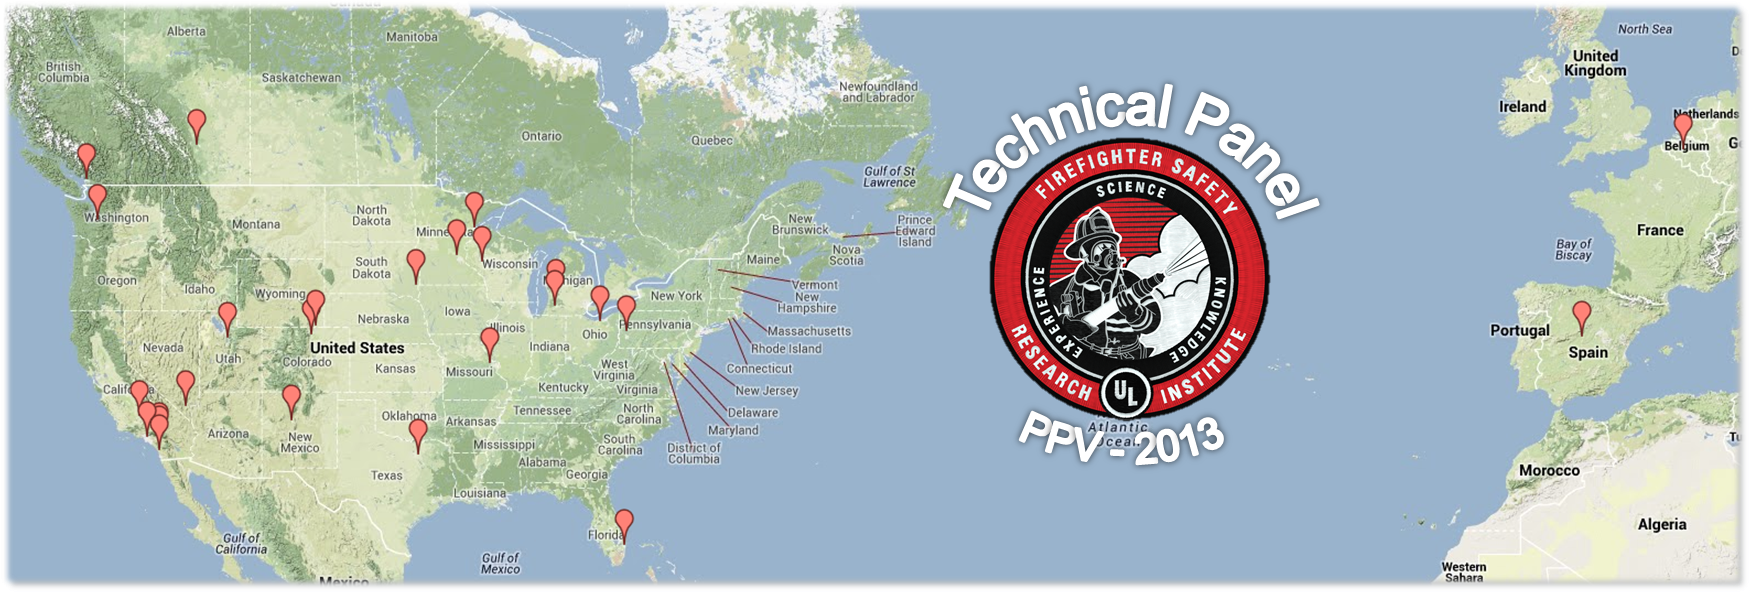
\includegraphics[width = 5in]{0_Images/Technical_Panel/TechnicalPanelLocations.png} 
	\caption{Positive Pressure Attack Technical Panel Member Locations}
	\label{fig:PanelLocatoins}
\end{figure} 

The individuals below provided direction for the project, assisting in planing the experiments, witnessing the testing and developing tactical considerations. Their tireless support and effort make this project relevant to the fire service across the world. 

\renewcommand{\arraystretch}{1.5}

\begin{table}[H]
	\centering
	\caption{Fire Service Technical Panel}
	\begin{tabular}{|c|c|}
		\hline
		\bf{Name} & \bf{Fire Department} \\ \hline \hline
		Art Armalich & CERN Labs Fire Department \\ \hline
		Jason Bennett & Poudre Fire Authority \\ \hline
		Ian Bolton & North Vancouver District Fire Services \\ \hline
		Jason Caughey & Laramie County Fire District \\ \hline
		Scott Corrigan & Pierce County Fire Department \\ \hline
		David Downey & Albuquerque Fire Department \\ \hline
		Chip Everett & Oshtemo Township Fire Department \\ \hline
		John Flynn & Palm Beach County Fire Rescue \\ \hline
		Adam Frick & Sioux Falls Fire Department \\ \hline
		Kriss Garcia & American Fork Fire Department \\ \hline
		Gregg Gerner & General Motors Assembly \\ \hline
		Jeff Gillette & East Valley Fire Department \\ \hline
		Jim Golondzinier & Los Angeles County Fire Department \\ \hline
		Andy Golz & Duluth Fire Department \\ \hline
		Dennis Haisma & Grand Rapids Fire Department (Ret.) \\ \hline
		Josh Janssen & Riverside County Fire Department \\ \hline
		Tom Jenkins & Rogers Fire Department \\ \hline
		Brian Kazmierzak & Penn Twp Fire Department \\ \hline
		Colin Kelley & Clark County Fire Department \\ \hline
		Karel Lambert & Brussels Fire Department \\ \hline
		Nick Ledin & Eau Claire Fire Department \\ \hline
		Scott Lindsay & Calgary Fire Department \\ \hline
		Joseph Pronesti & Elyria Fire Department \\ \hline
		Garrett Rice & Colony Fire Department \\ \hline
		Ned Vander Pol & Vista Fire Department \\ \hline
	\end{tabular}
	\label{tab:TechPanelList}
\end{table}

\section{Ventilation Limited Room Experiments}
A fire releases energy in direct proportion to the amount of available oxygen. Past studies conducted under the Department of Homeland Security's Assistance to Firefighters Grant Program have established a basis of this for both single compartment fires along with fires within a residential structure \cite{DHS2008} \cite{DHS2010}. In order to provide further understanding of this concept, two, room scale experiments were conducted under a cone calorimeter hood to evaluate the energy release rate as it compares to the fuel load in a furnished compartment as compared to an overfurnished compartment with the same ventilation opening.

Each compartment measured 12ft long by 12ft wide and 8ft tall, with a front opening of 7ft - 10$\frac{3}{4}$in wide by 8ft high. The walls were wood stud frame 16in on center covered with $\frac{1}{2}$in type X gypsum wall board. The ceiling was supported by 2in x 6in framing 16in on center covered with a type X gypsum wall board. The floor was concrete covered with a $\frac{1}{2}$in cement board. The compartments were constructed side by side in the oxygen consumption calorimeter lab at UL's Northbrook test facility. 

\paragraph{Furnished Compartment} \mbox{}

The furnished compartment contained a sofa, arm chair, coffee table, TV Stand, tube television, two plastic bins, two end tables, lamp, stuffed toys, picture frames, candles, drapes, and a polyester carpet with foam padding. See Figure \ref{fig:furnished_images} for arrangement of furnishings.

\begin{figure}[H]
	\centering
	\begin{tabular} {c c c}
	\subfloat[]{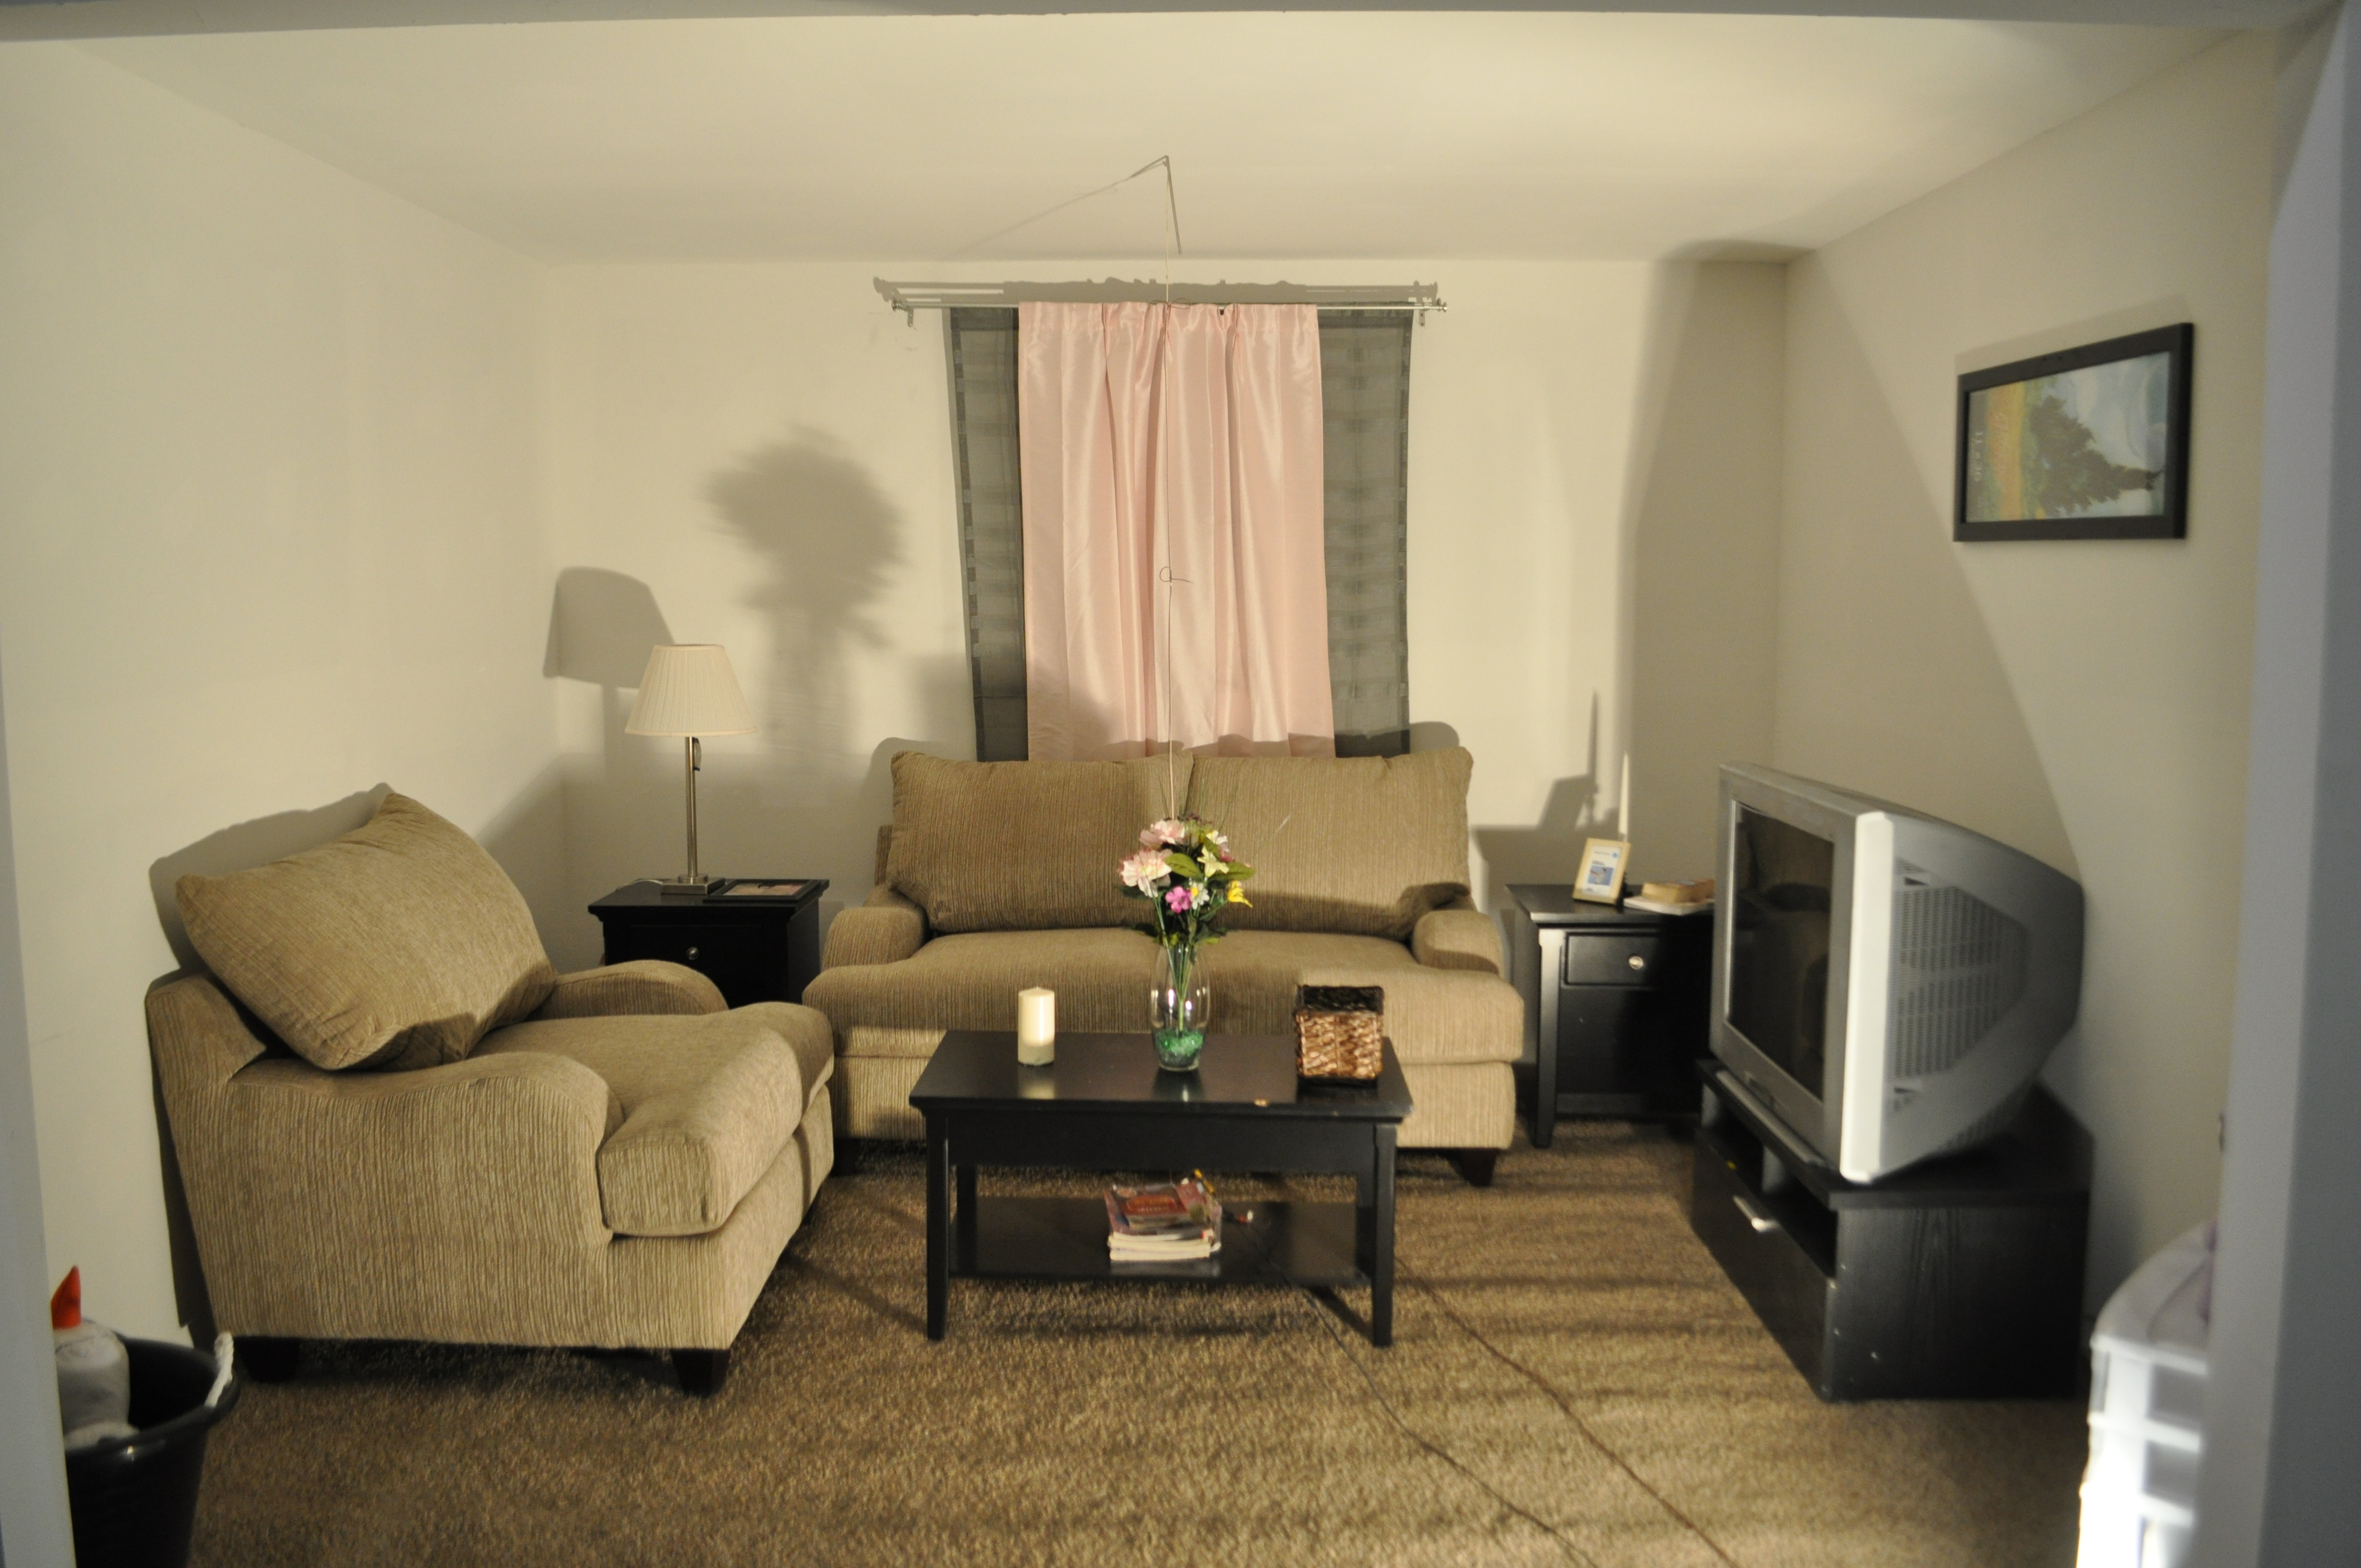
\includegraphics[width=5cm]{0_Images/Vent_Limited_Room/Furnished_Overall.jpg}} &
	\subfloat[]{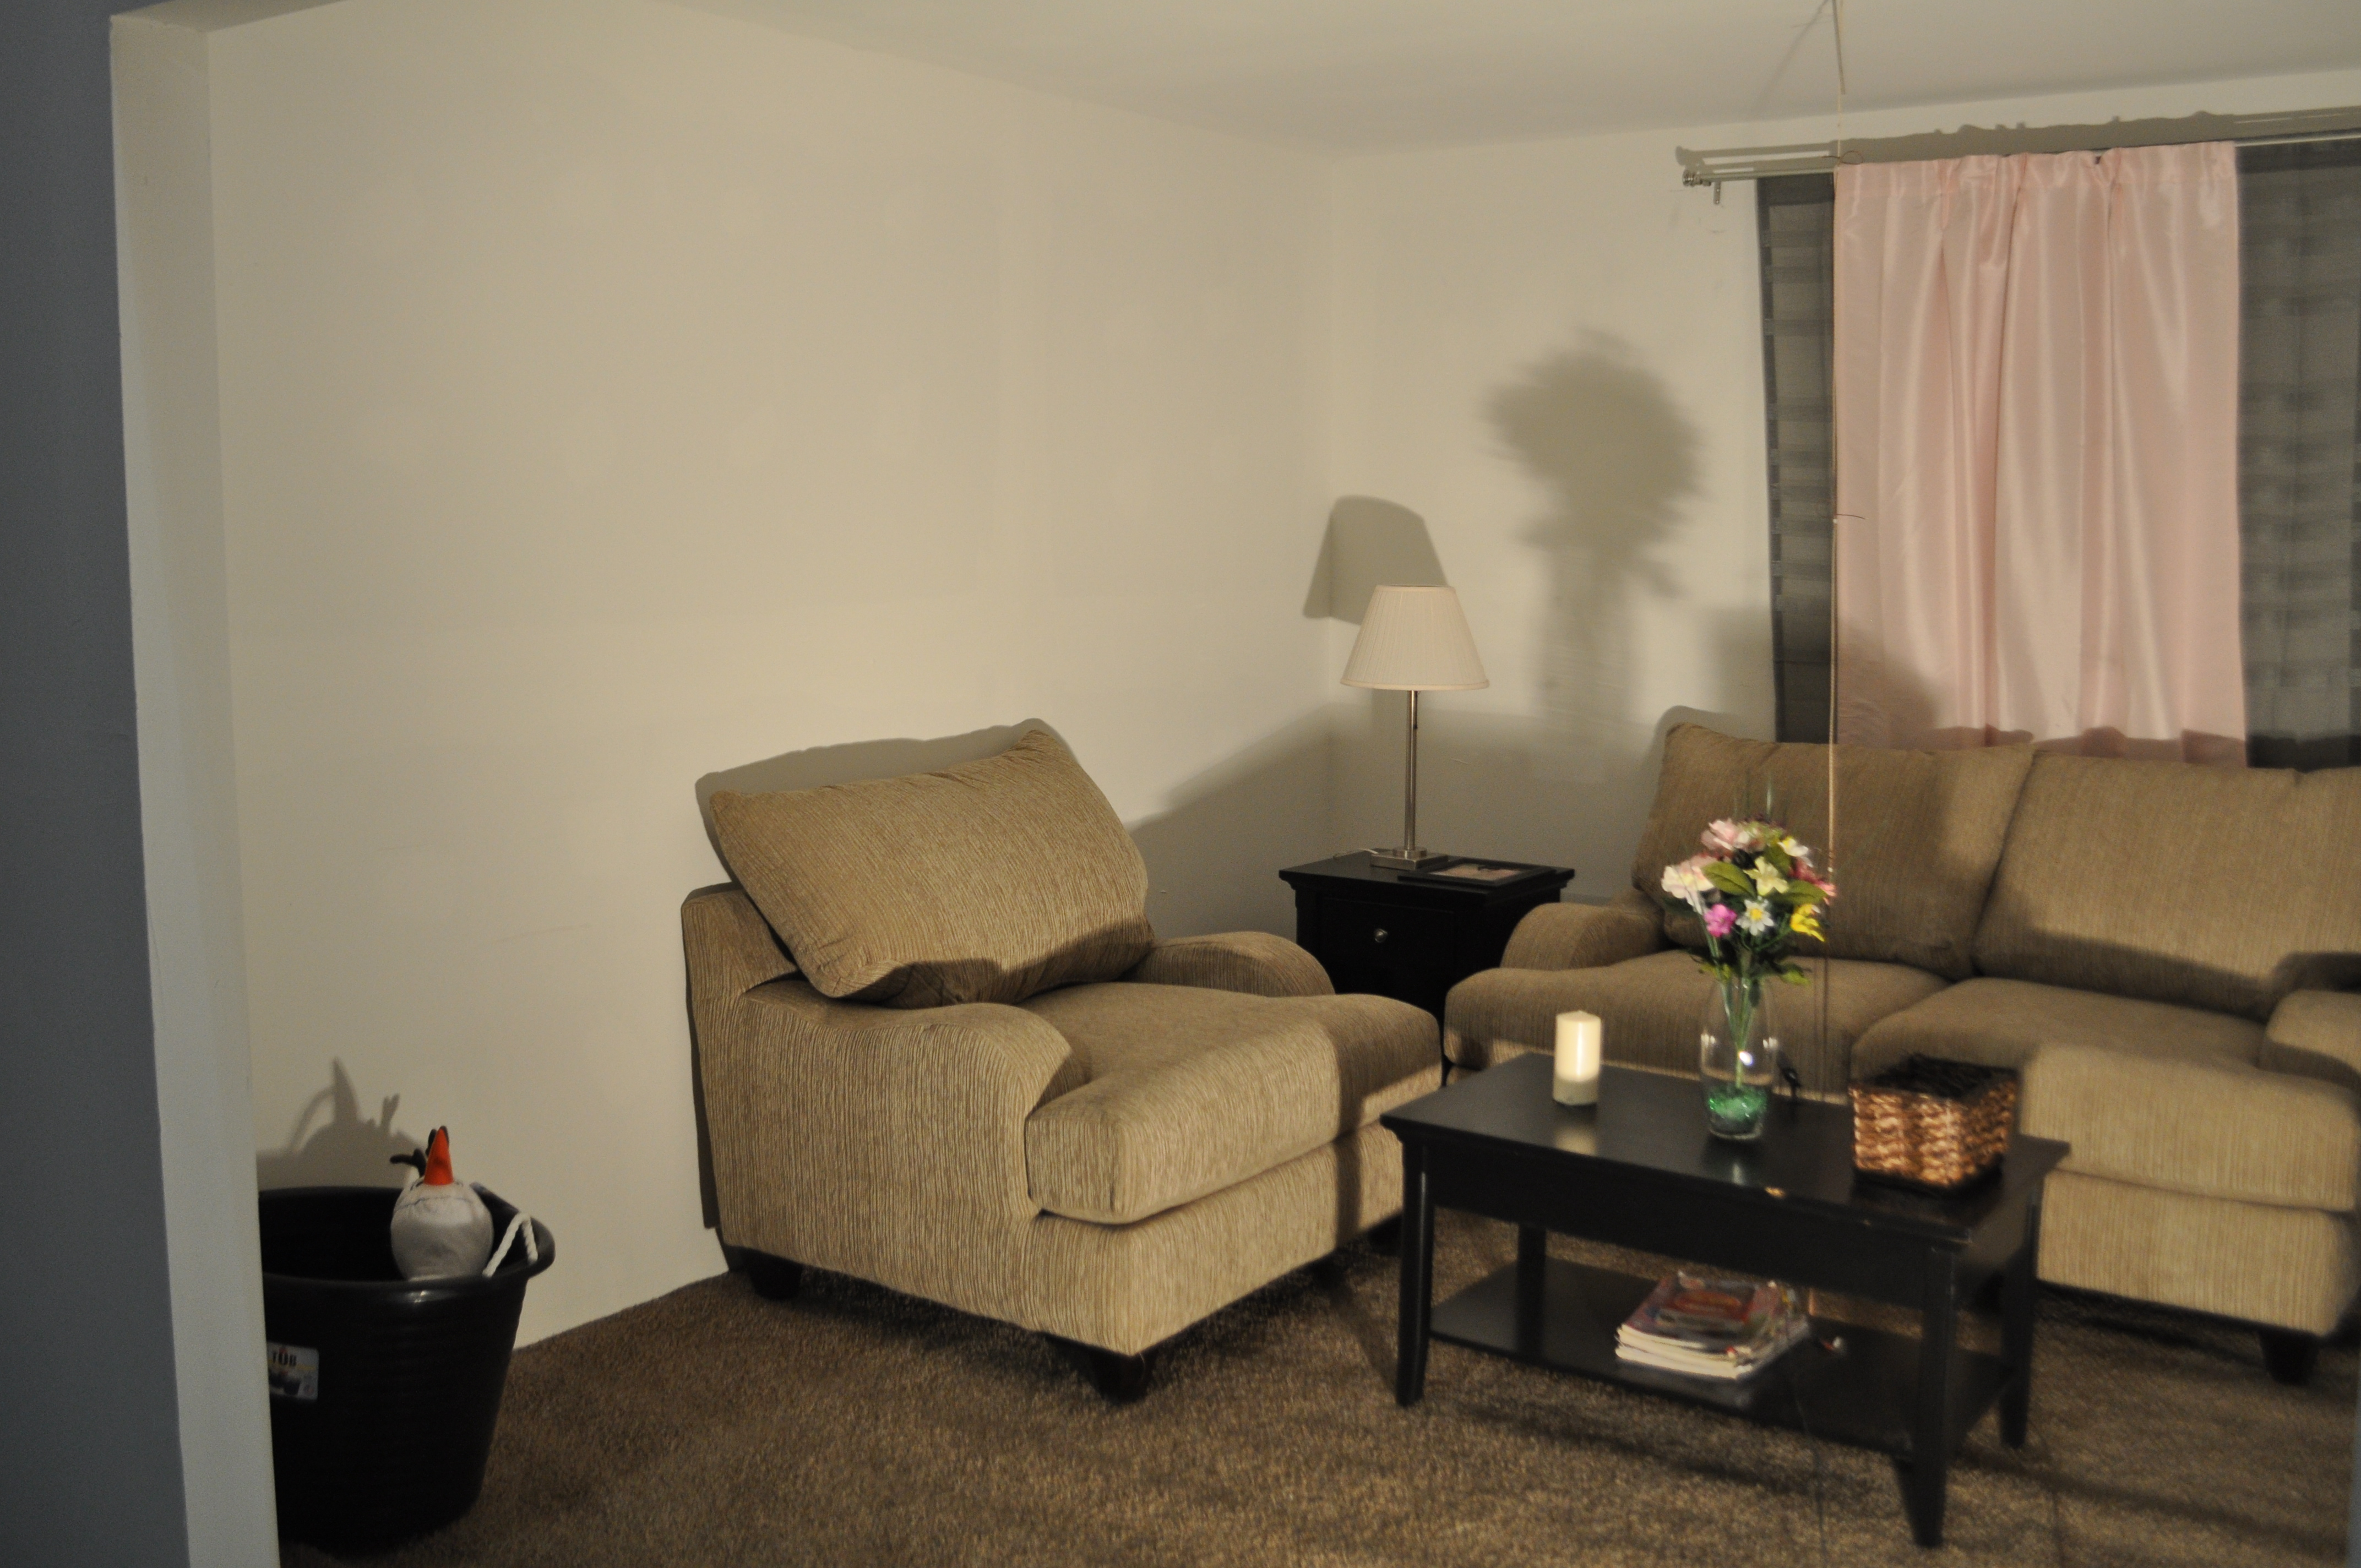
\includegraphics[width=5cm]{0_Images/Vent_Limited_Room/Furnished_Left_Side.jpg}} &
	\subfloat[]{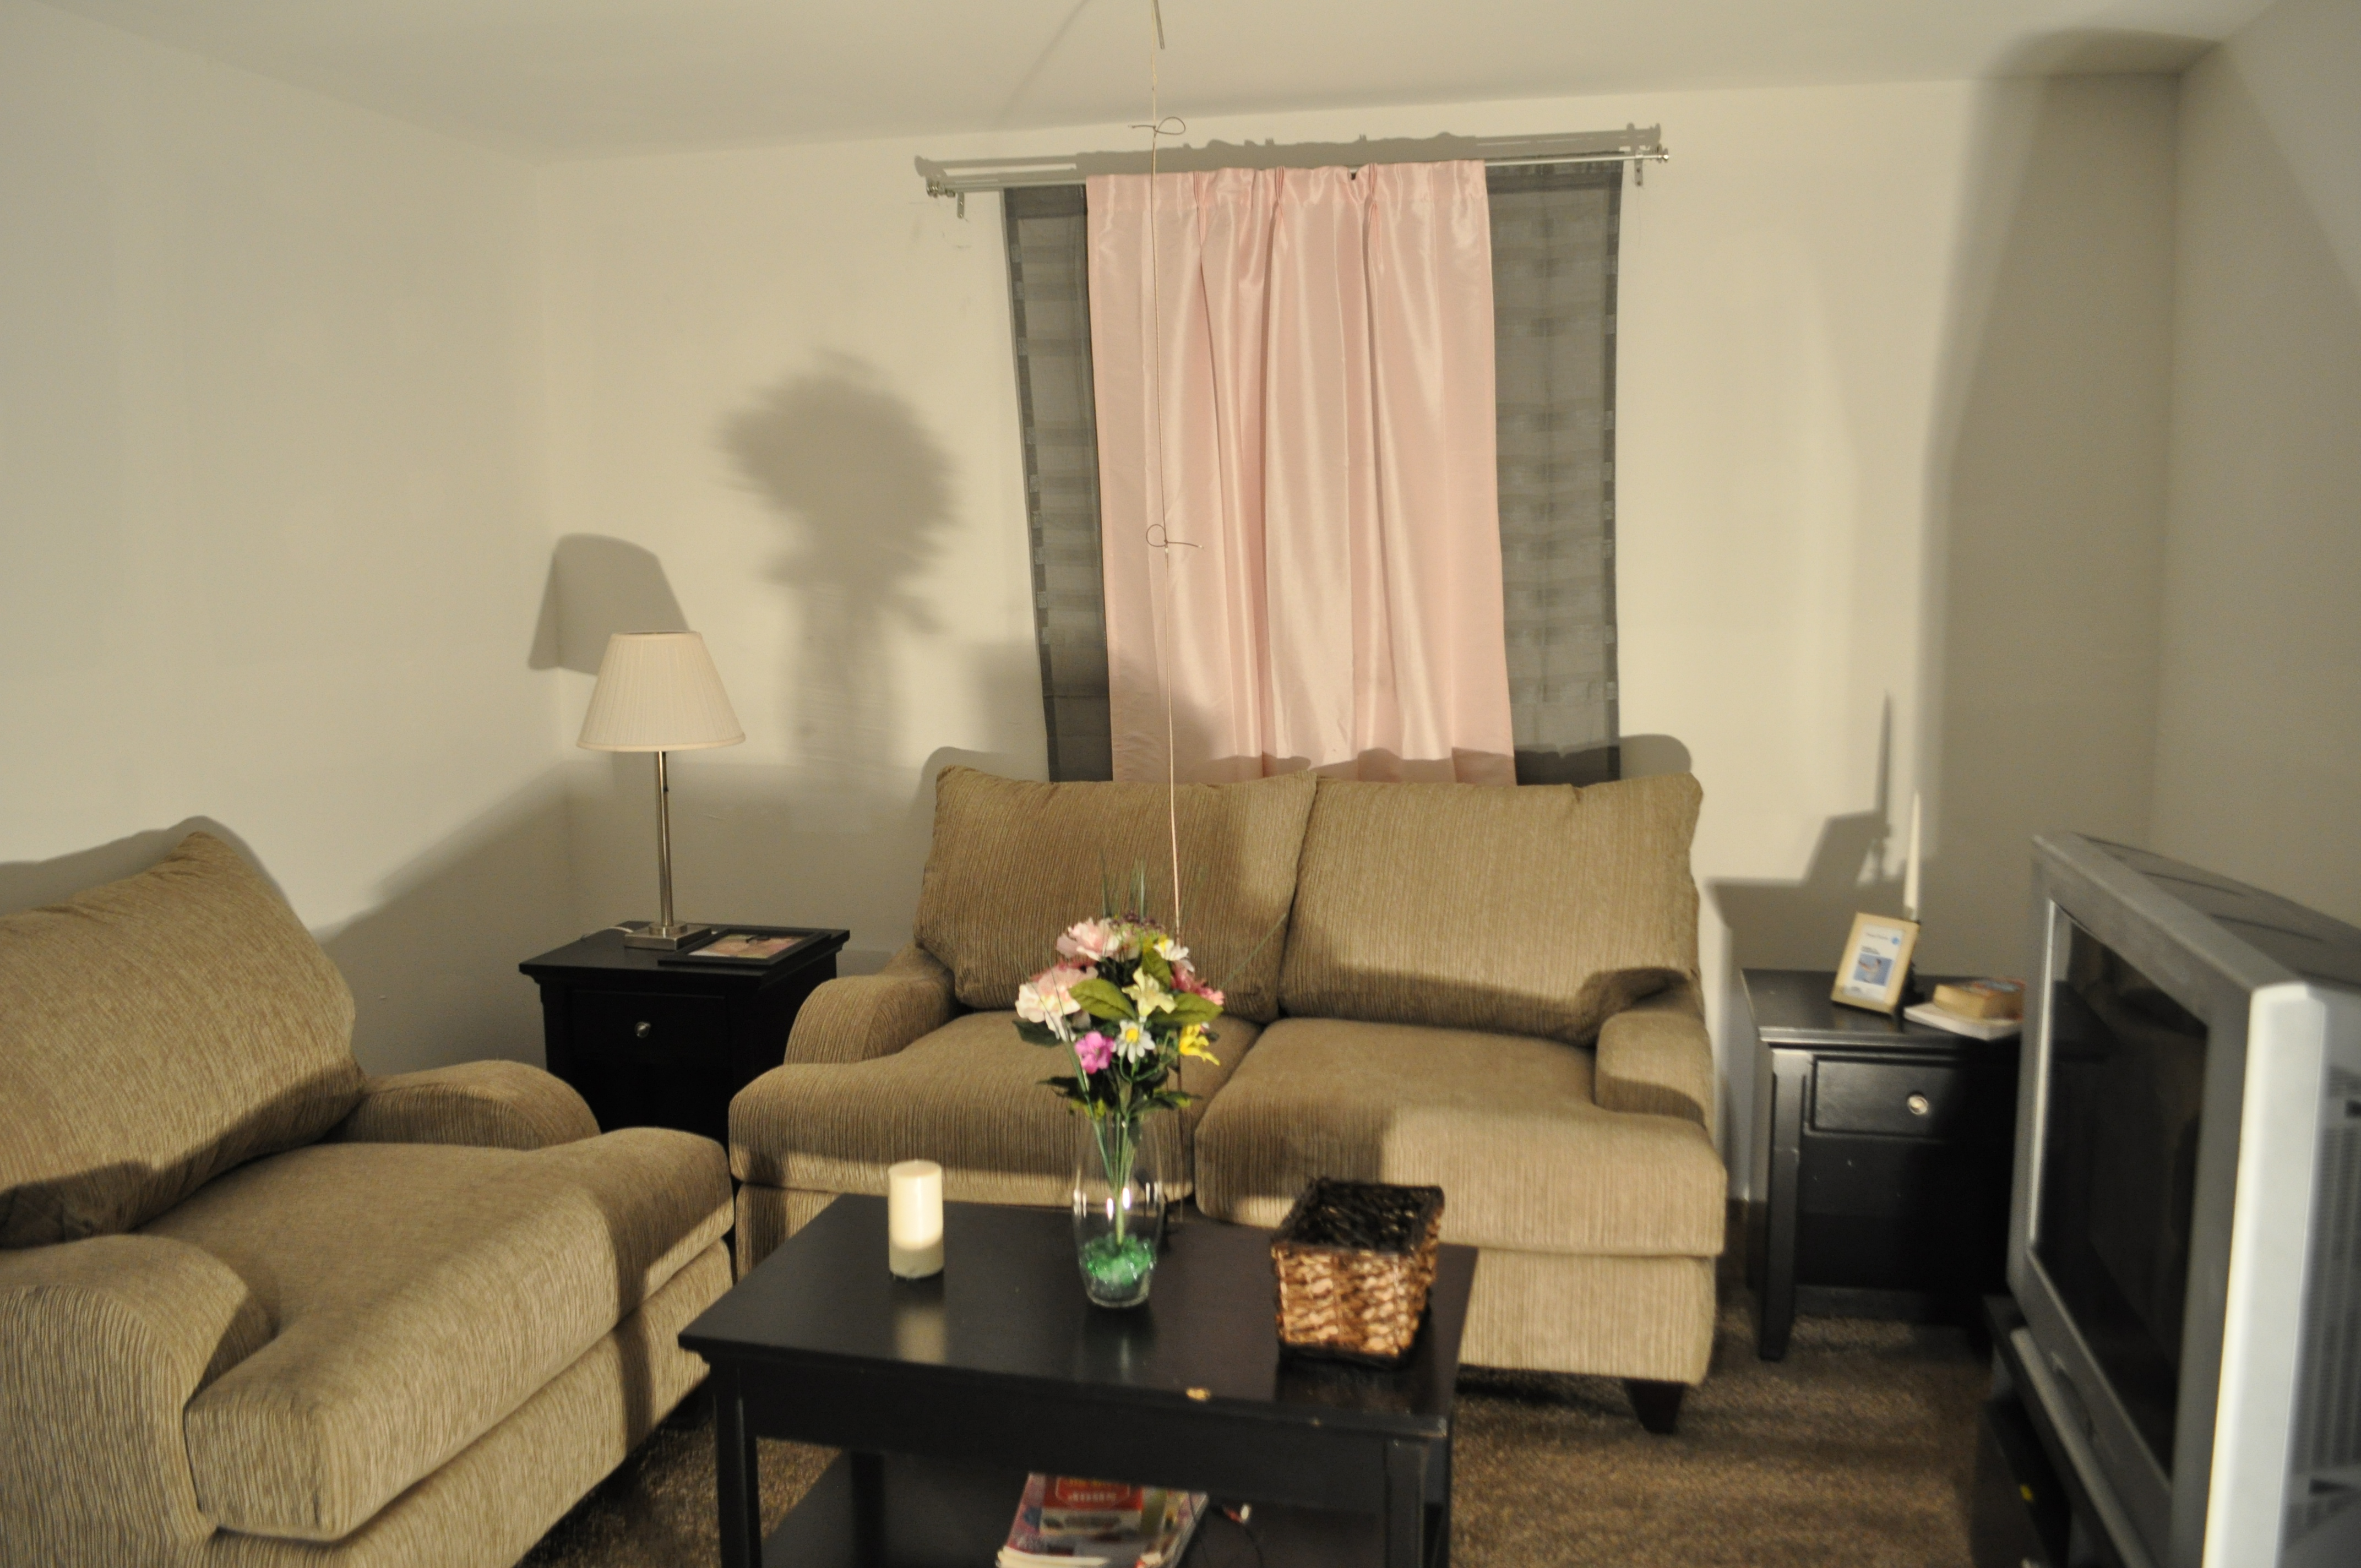
\includegraphics[width=5cm]{0_Images/Vent_Limited_Room/Furnished_Center.jpg}} \\
	\end{tabular}
	\begin{tabular} { c c }
	\subfloat[]{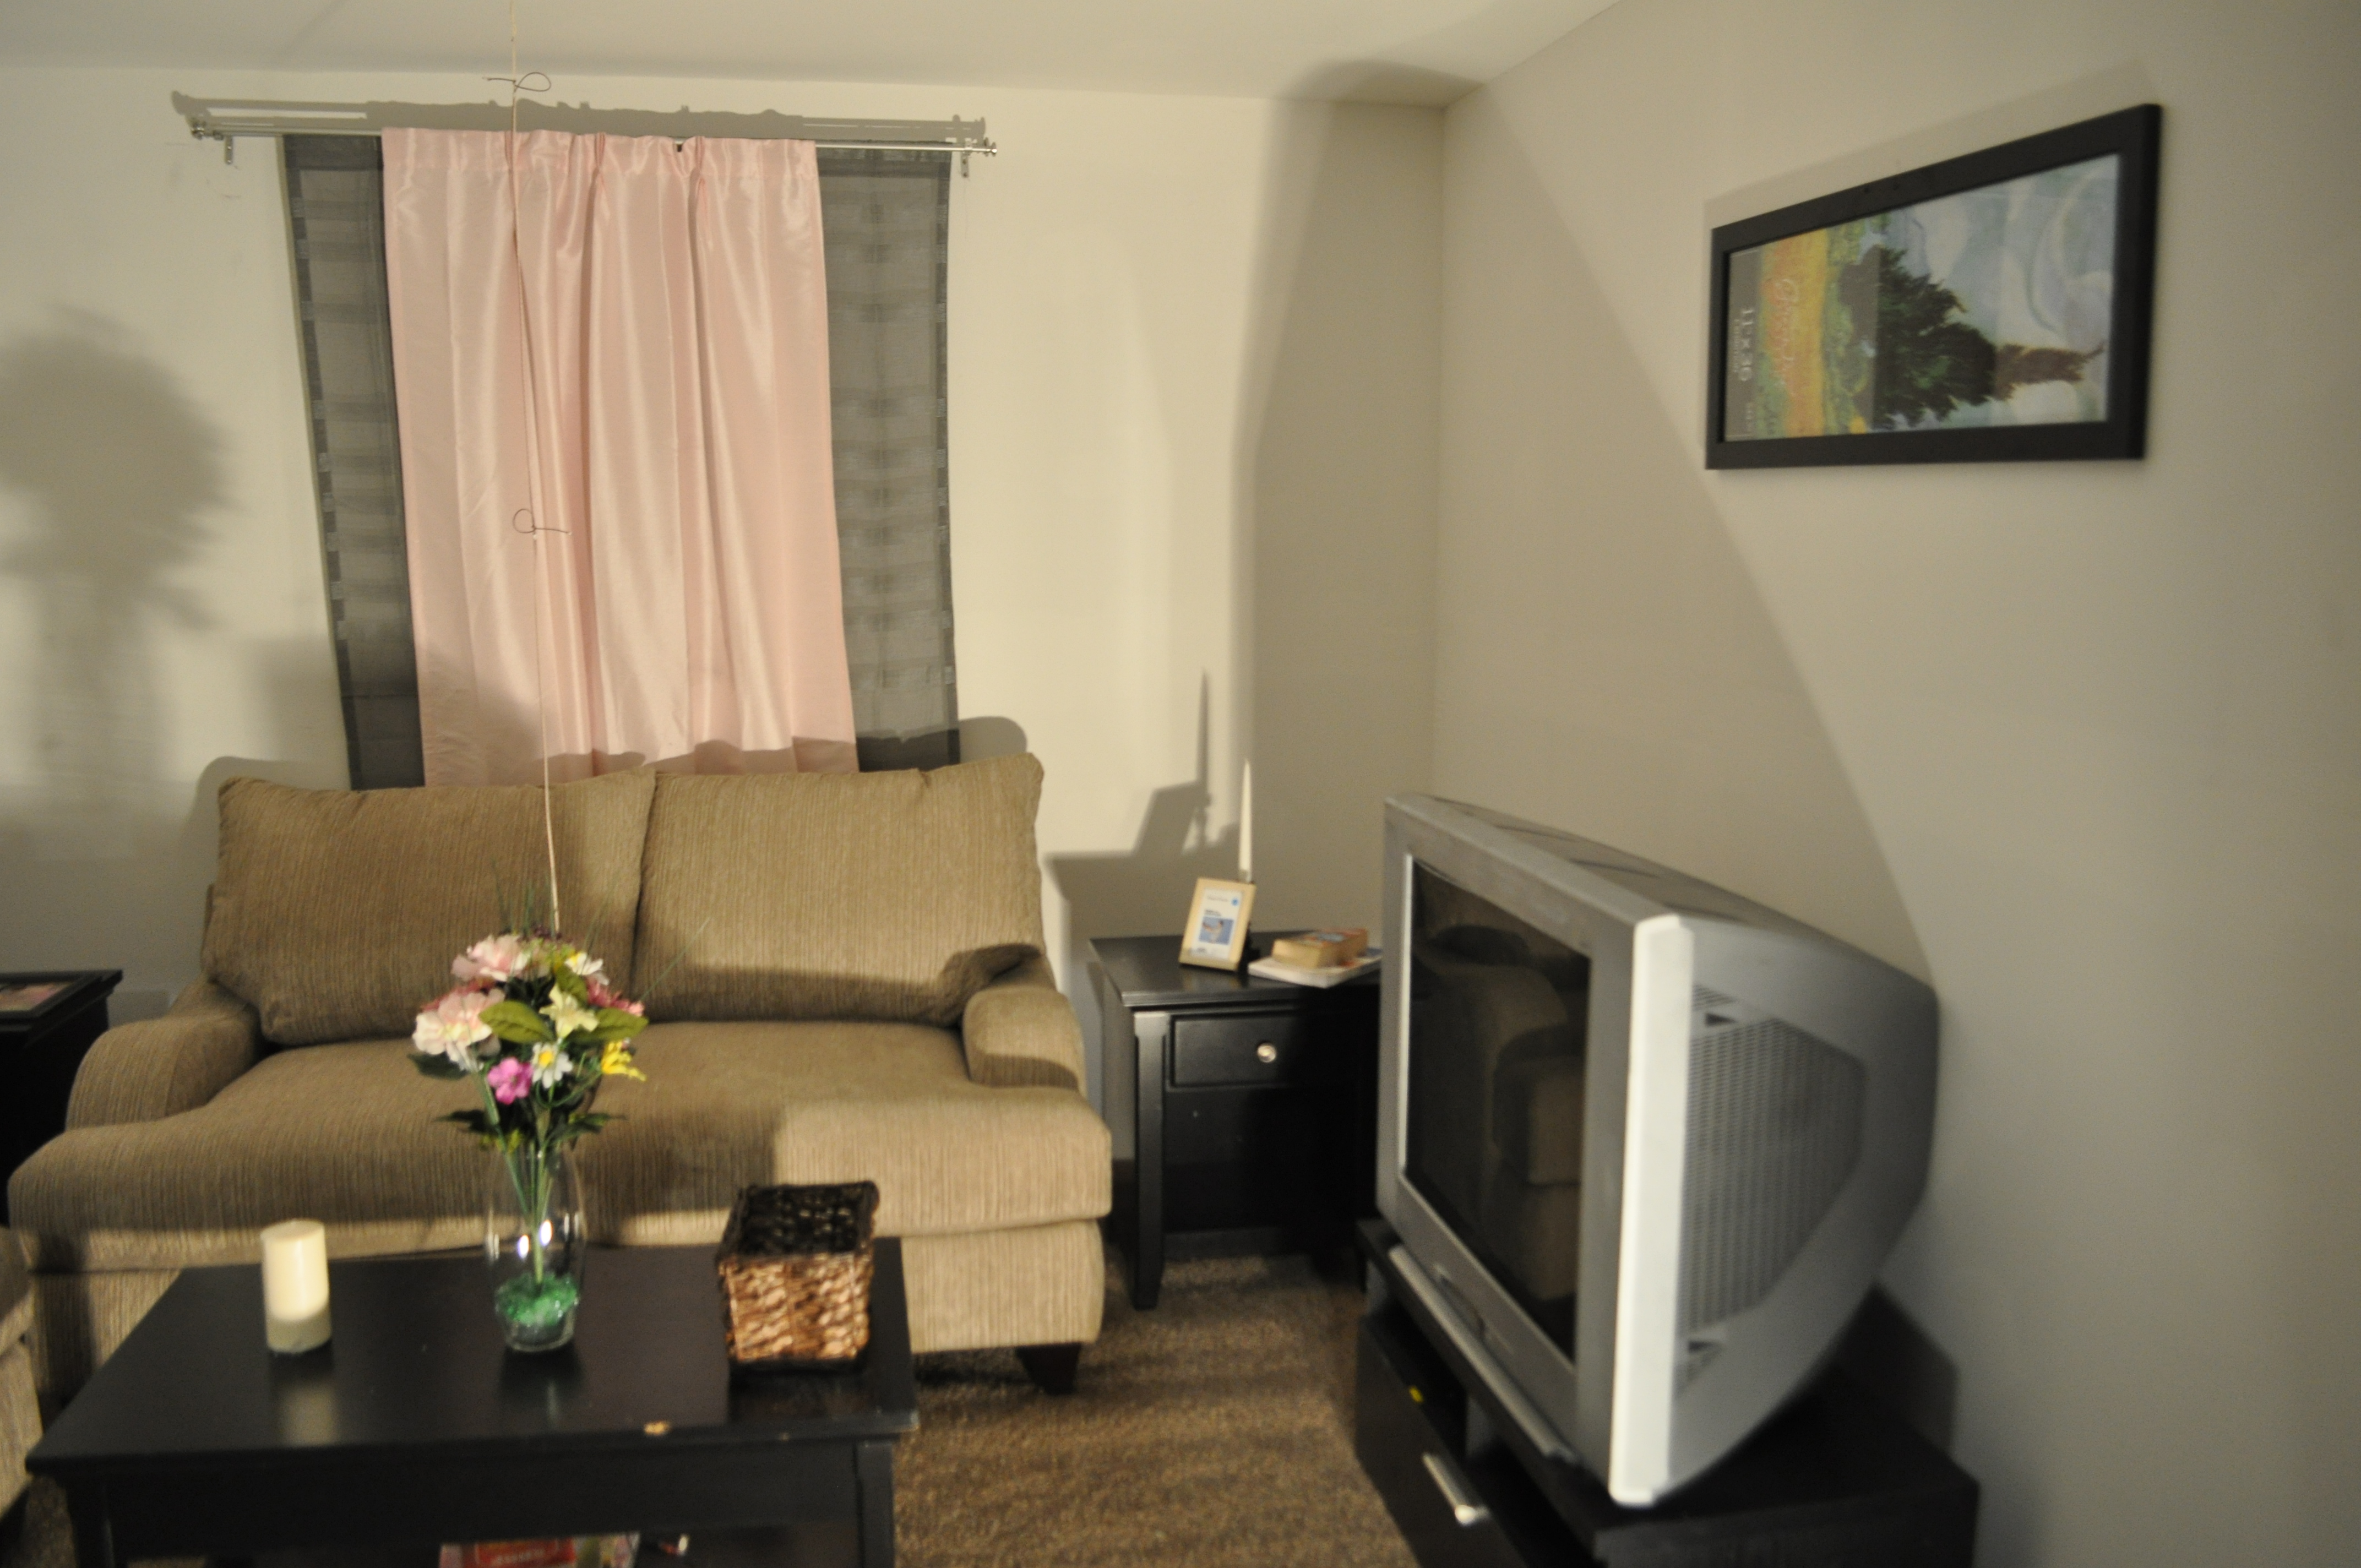
\includegraphics[width=5cm]{0_Images/Vent_Limited_Room/Furnished_Center_Right.jpg}} &
	\subfloat[]{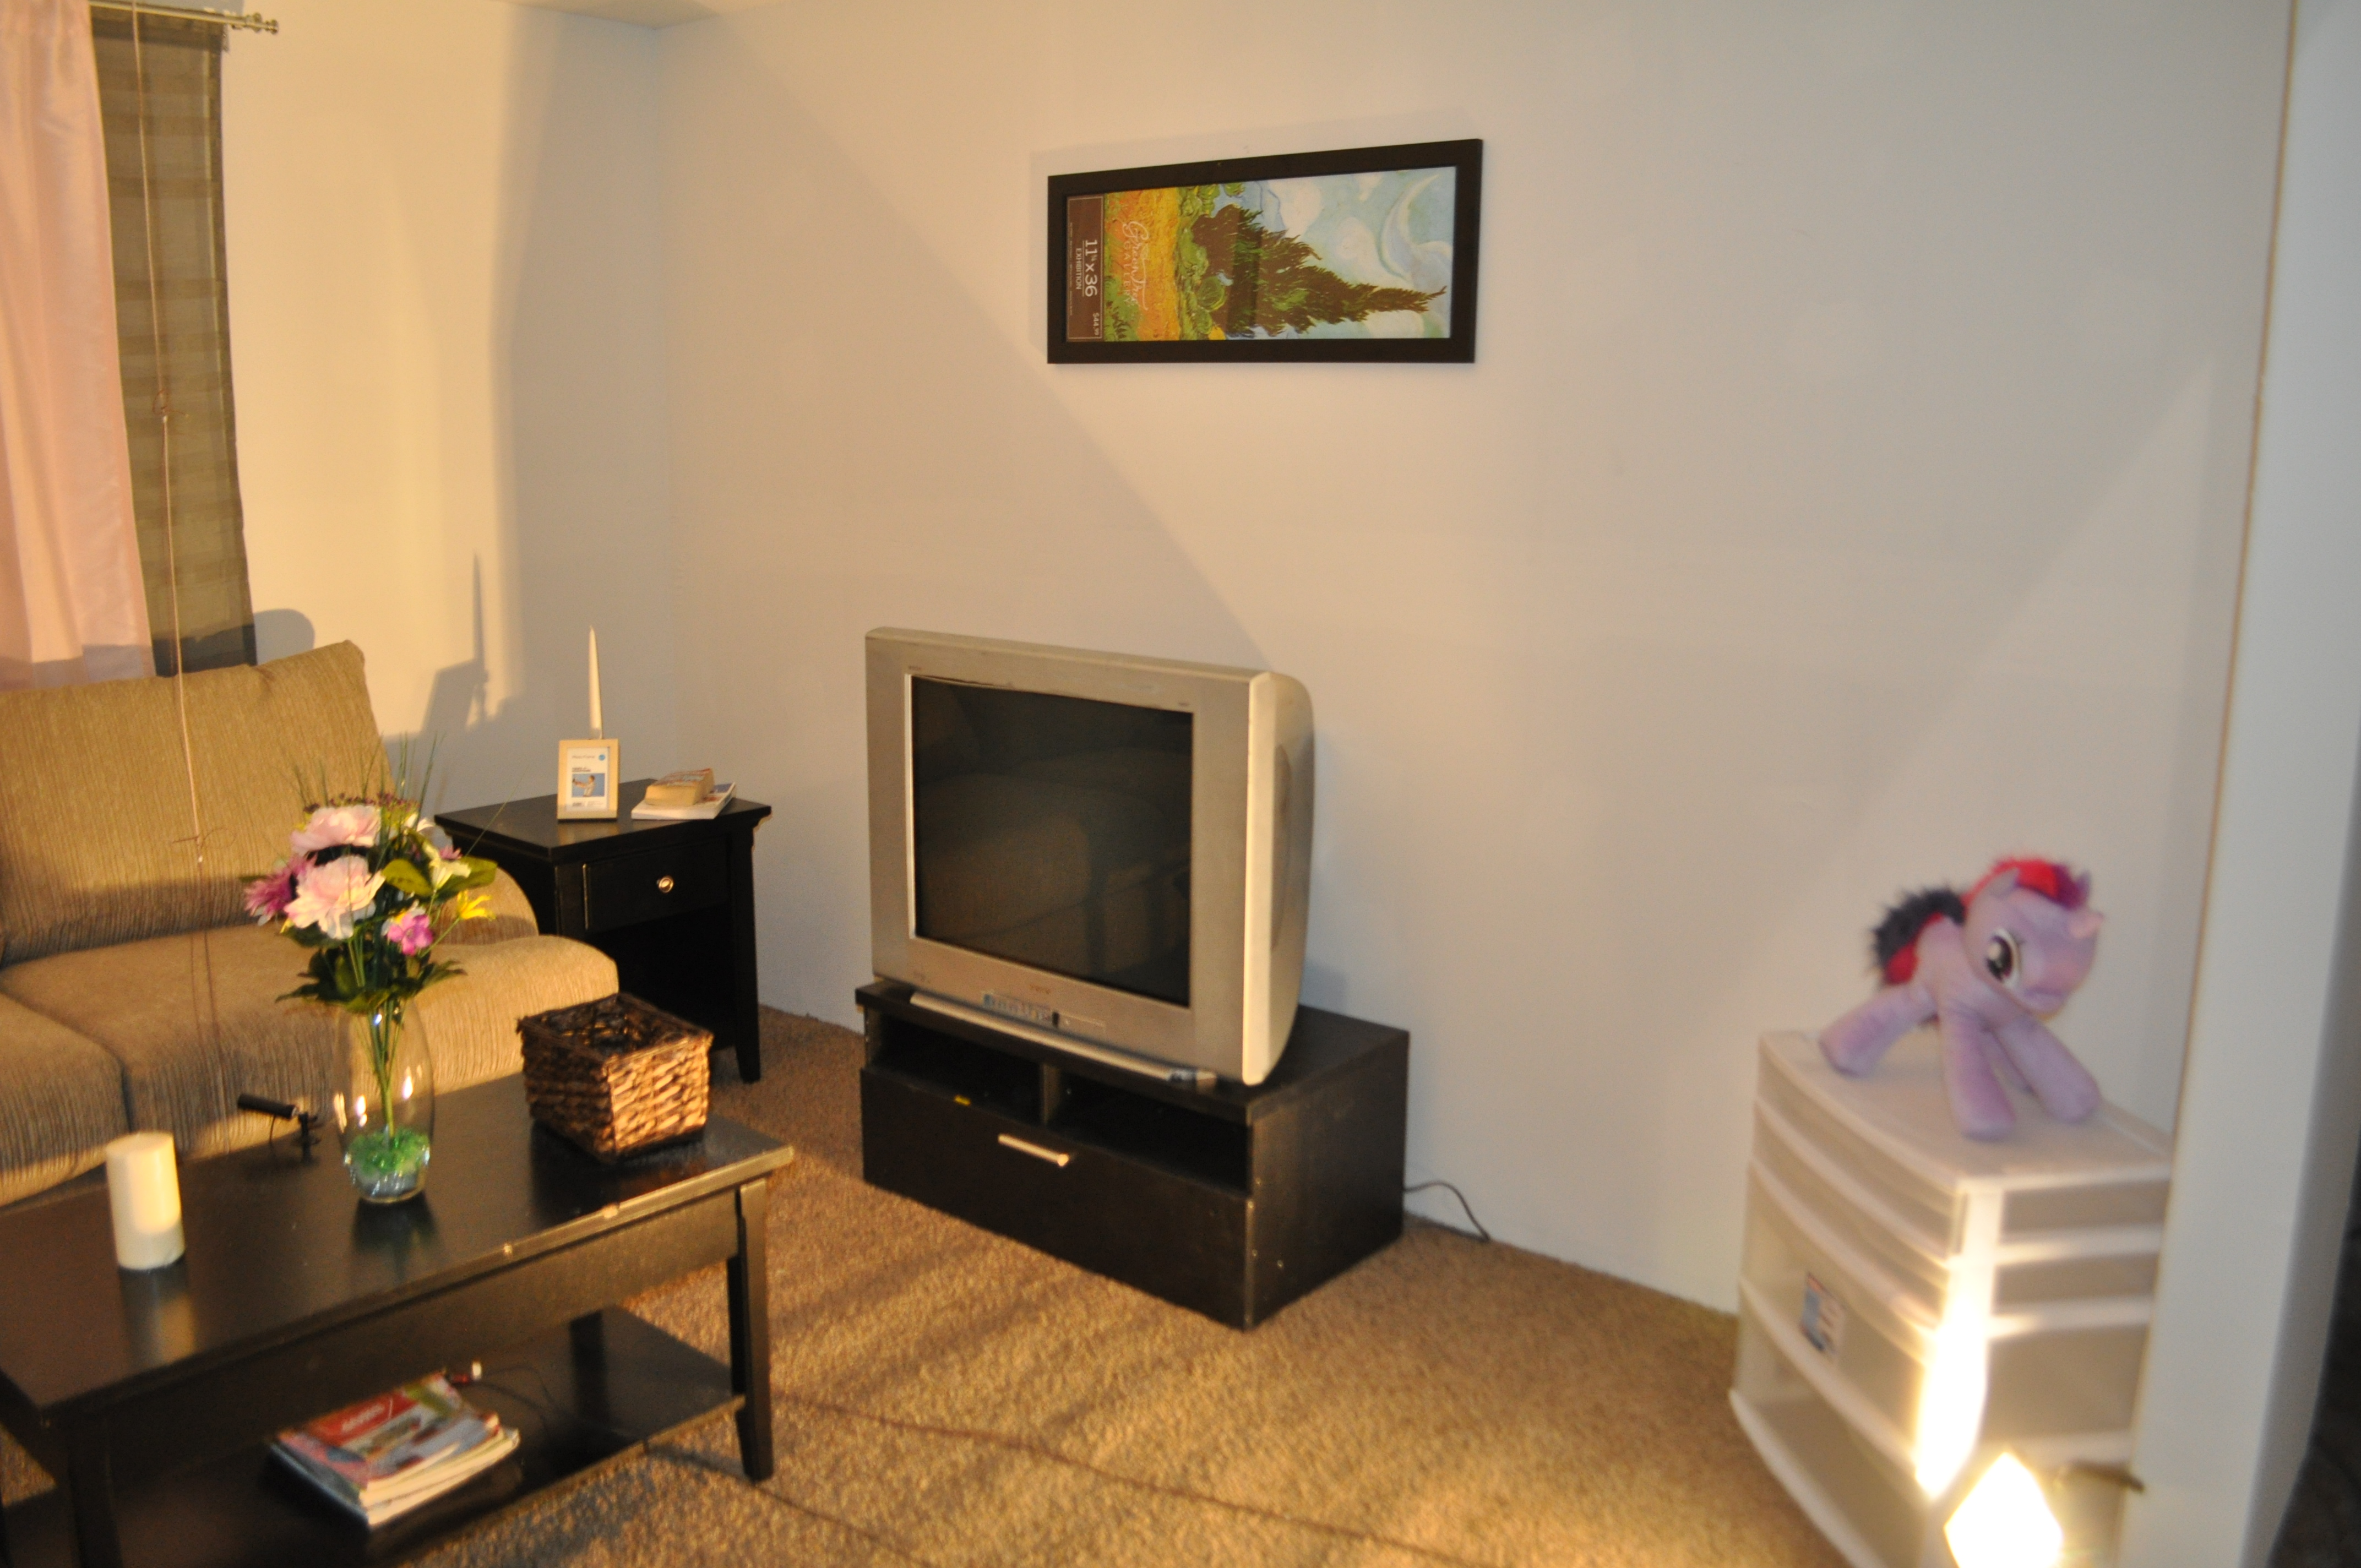
\includegraphics[width=5cm]{0_Images/Vent_Limited_Room/Furnished_Right_Side.jpg}} \\
	\end{tabular}
	\caption{Furnished Room Images}
	\label{fig:furnished_images}
\end{figure}

\paragraph{Over Furnished Compartment} \mbox{}

The over furnished compartment contained six stuffed brown chairs, two orange sleeper sofas and two one green sleeper sofa from the furniture aquired for the full scale fire experiments. The furniture was arranged as shown in Figure \ref{fig:horder_images}.

\begin{figure}[H]
	\centering
	\begin{tabular} {c c c}
		\subfloat[]{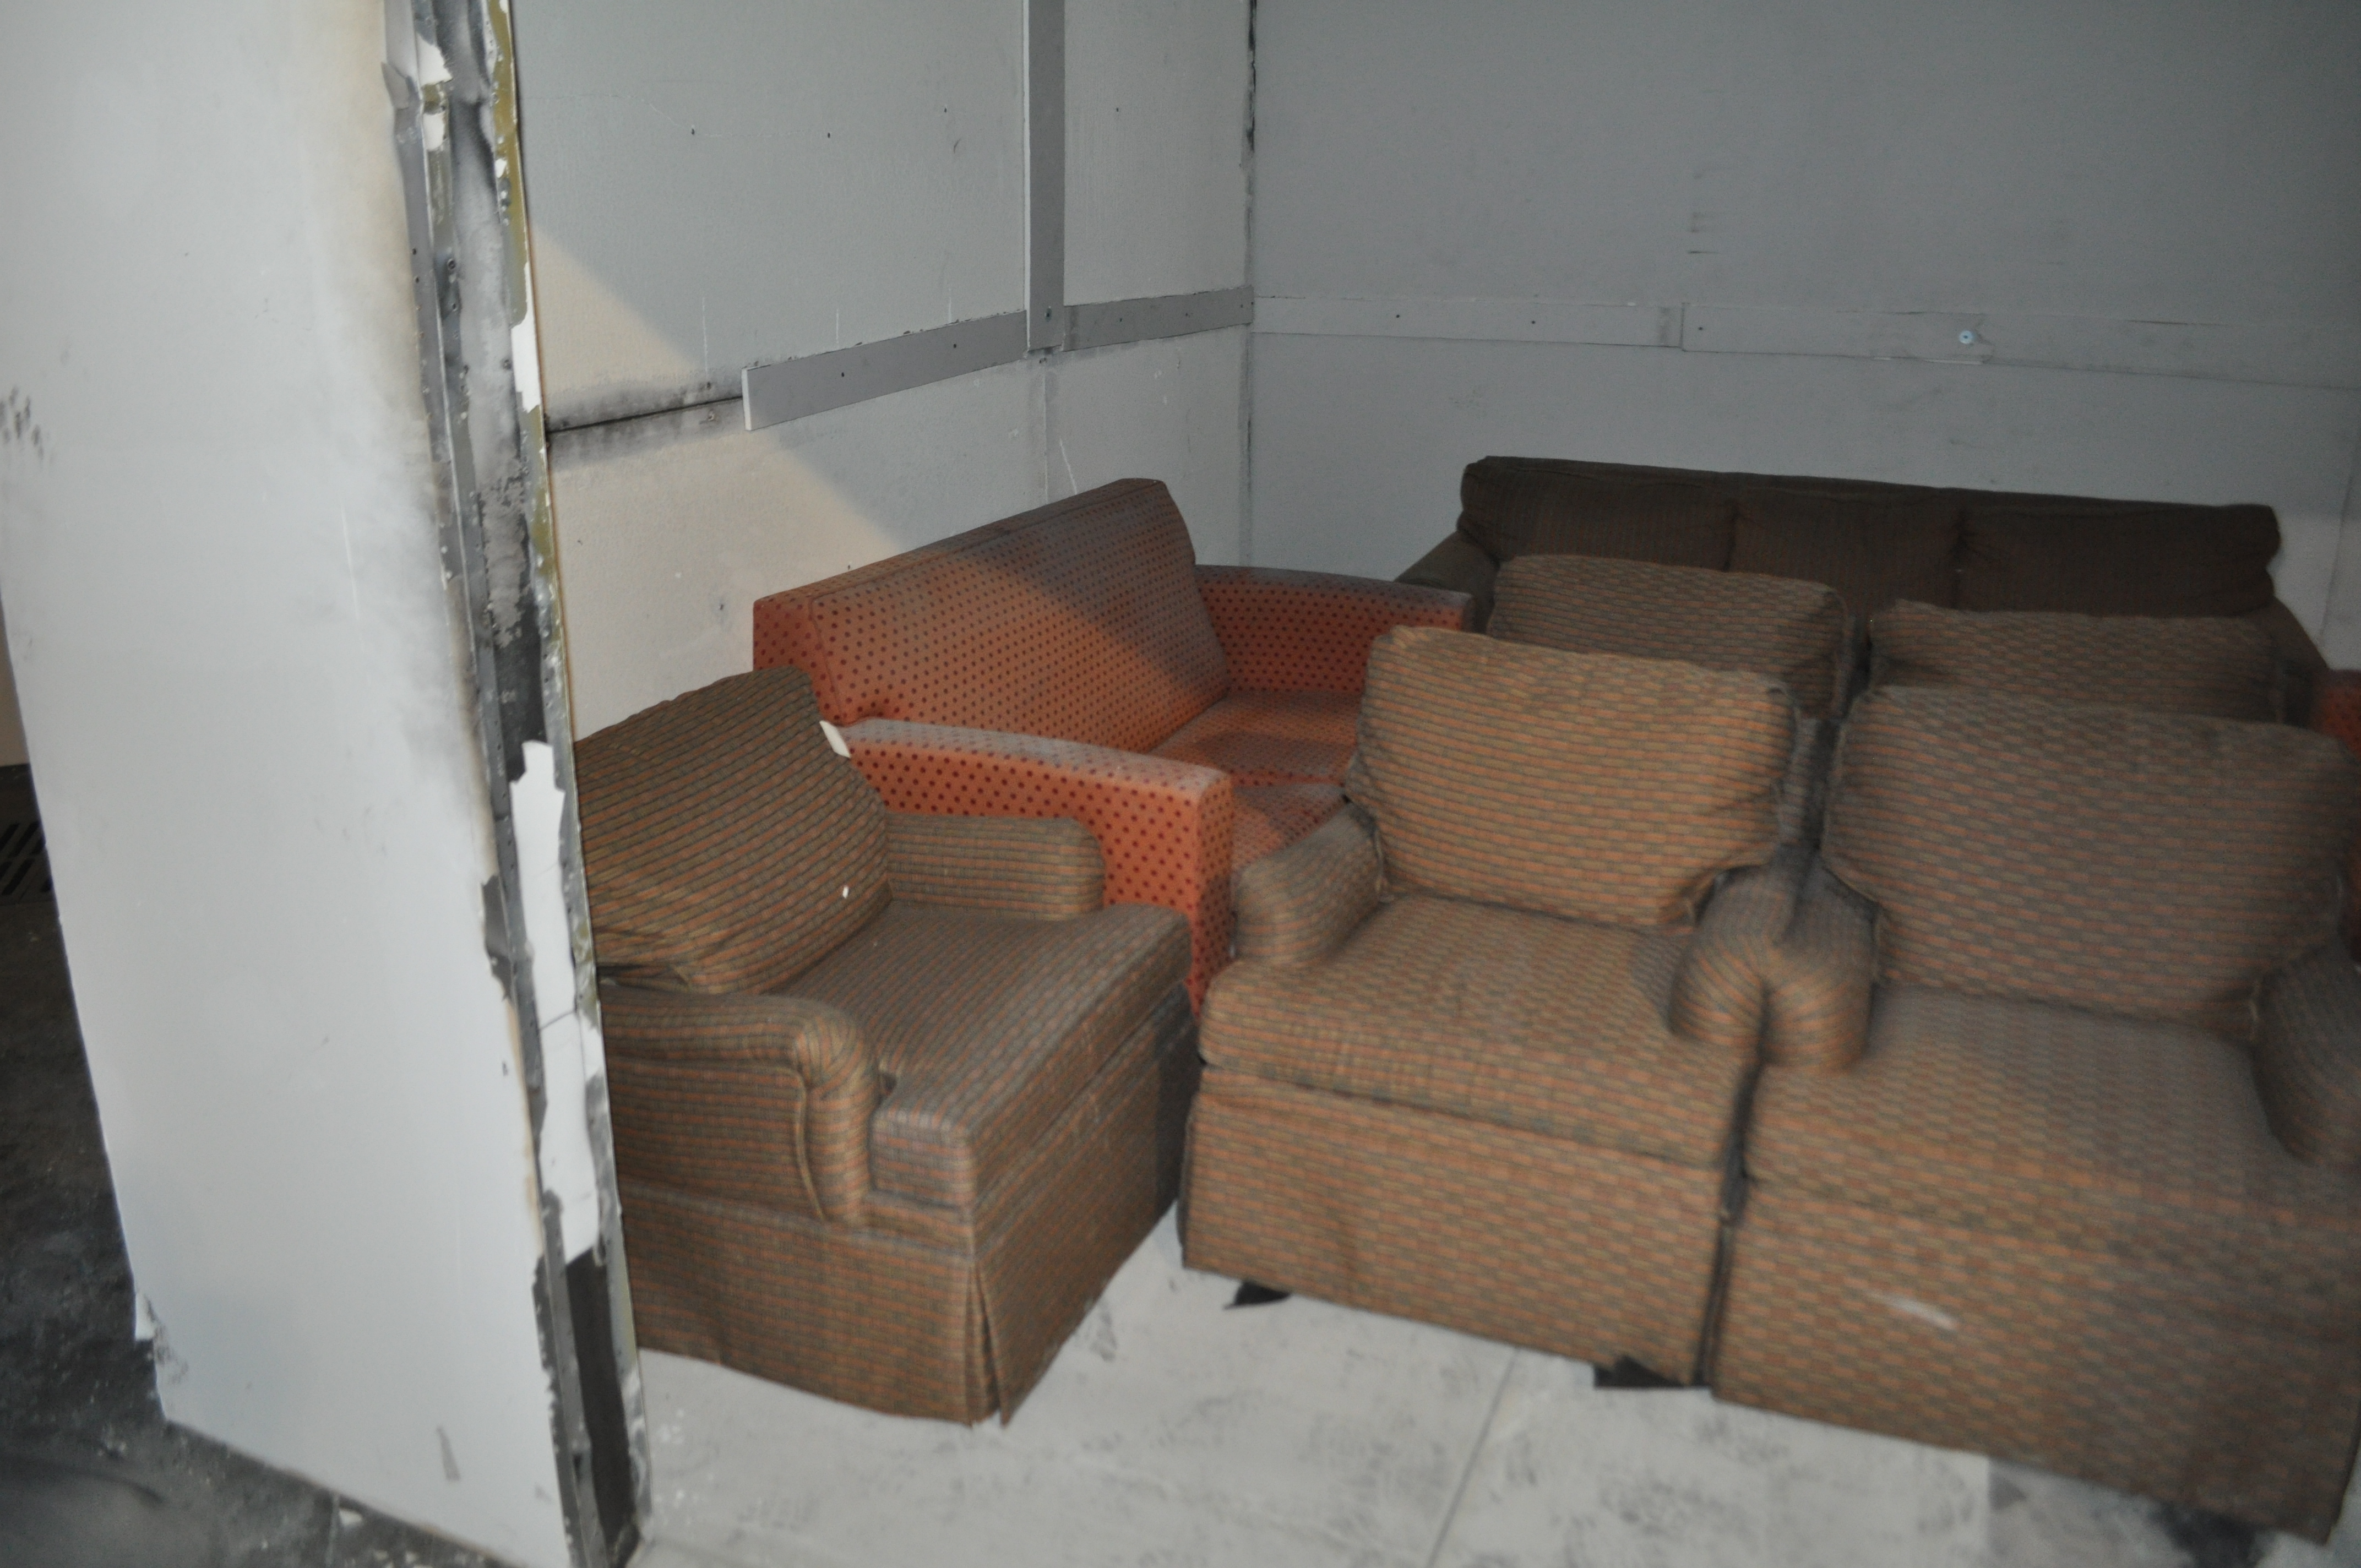
\includegraphics[width=5cm]{0_Images/Vent_Limited_Room/Horder1.jpg}} &
		\subfloat[]{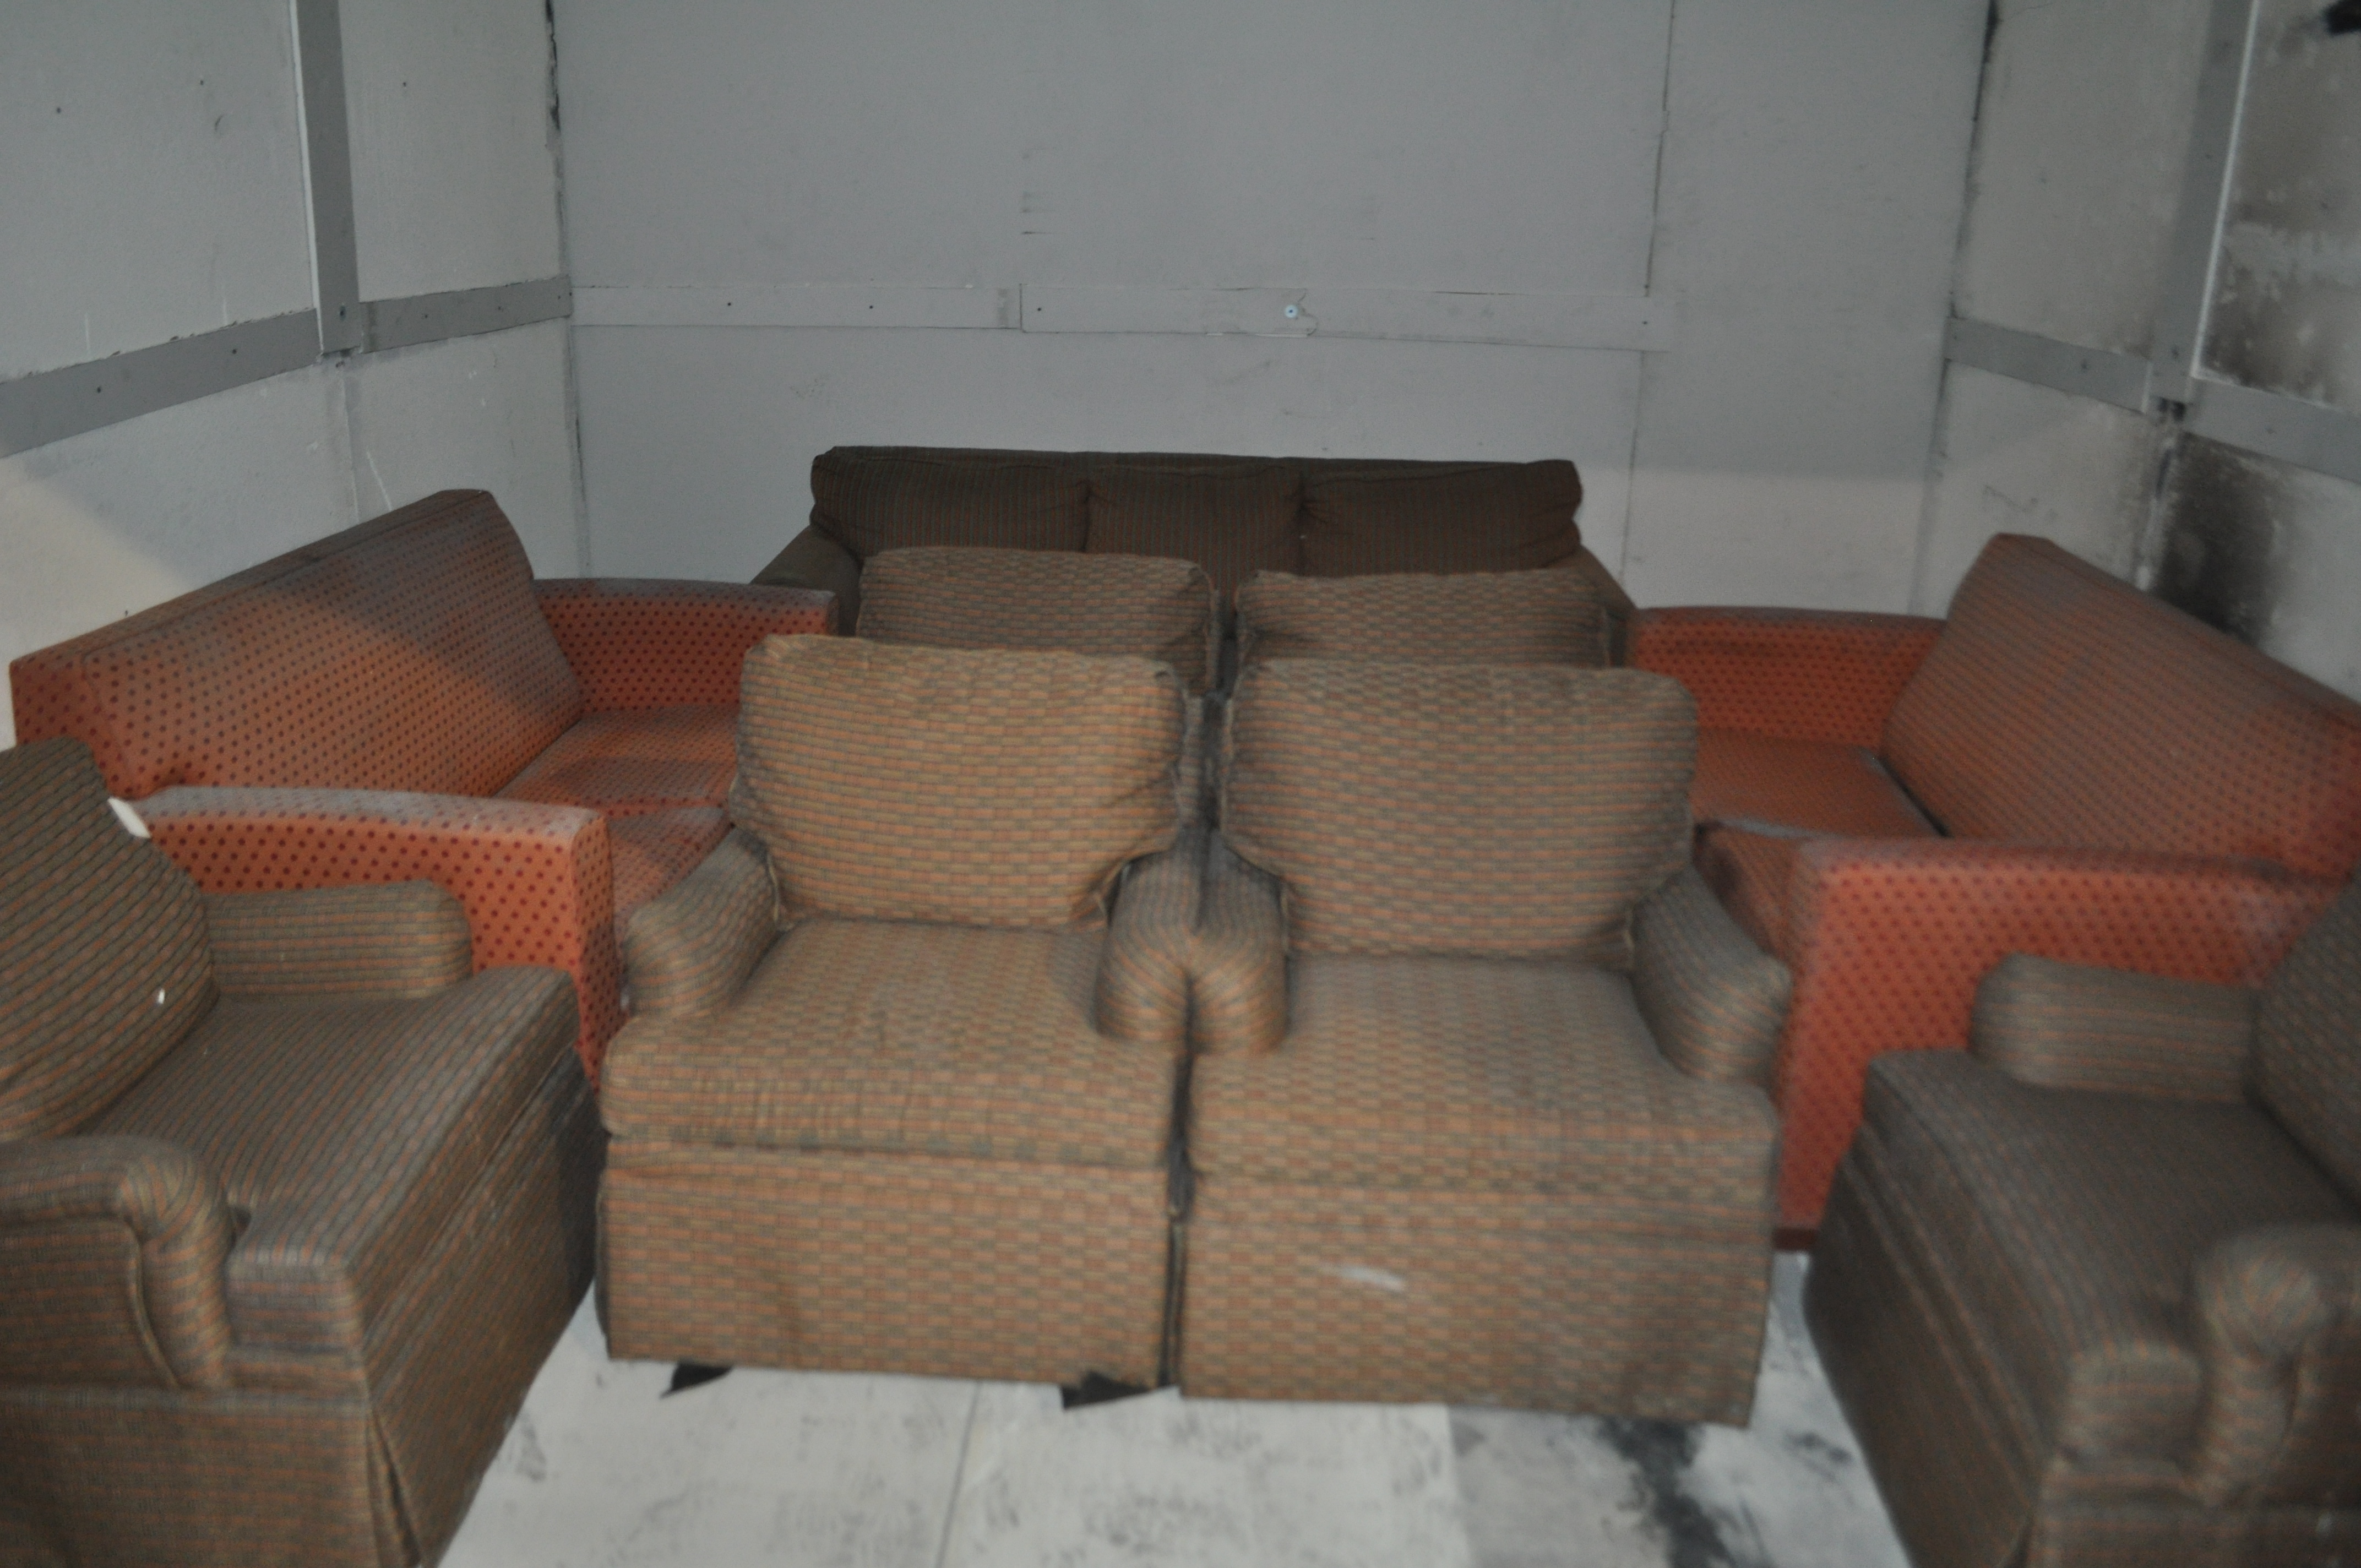
\includegraphics[width=5cm]{0_Images/Vent_Limited_Room/Horder2.jpg}} &
		\subfloat[]{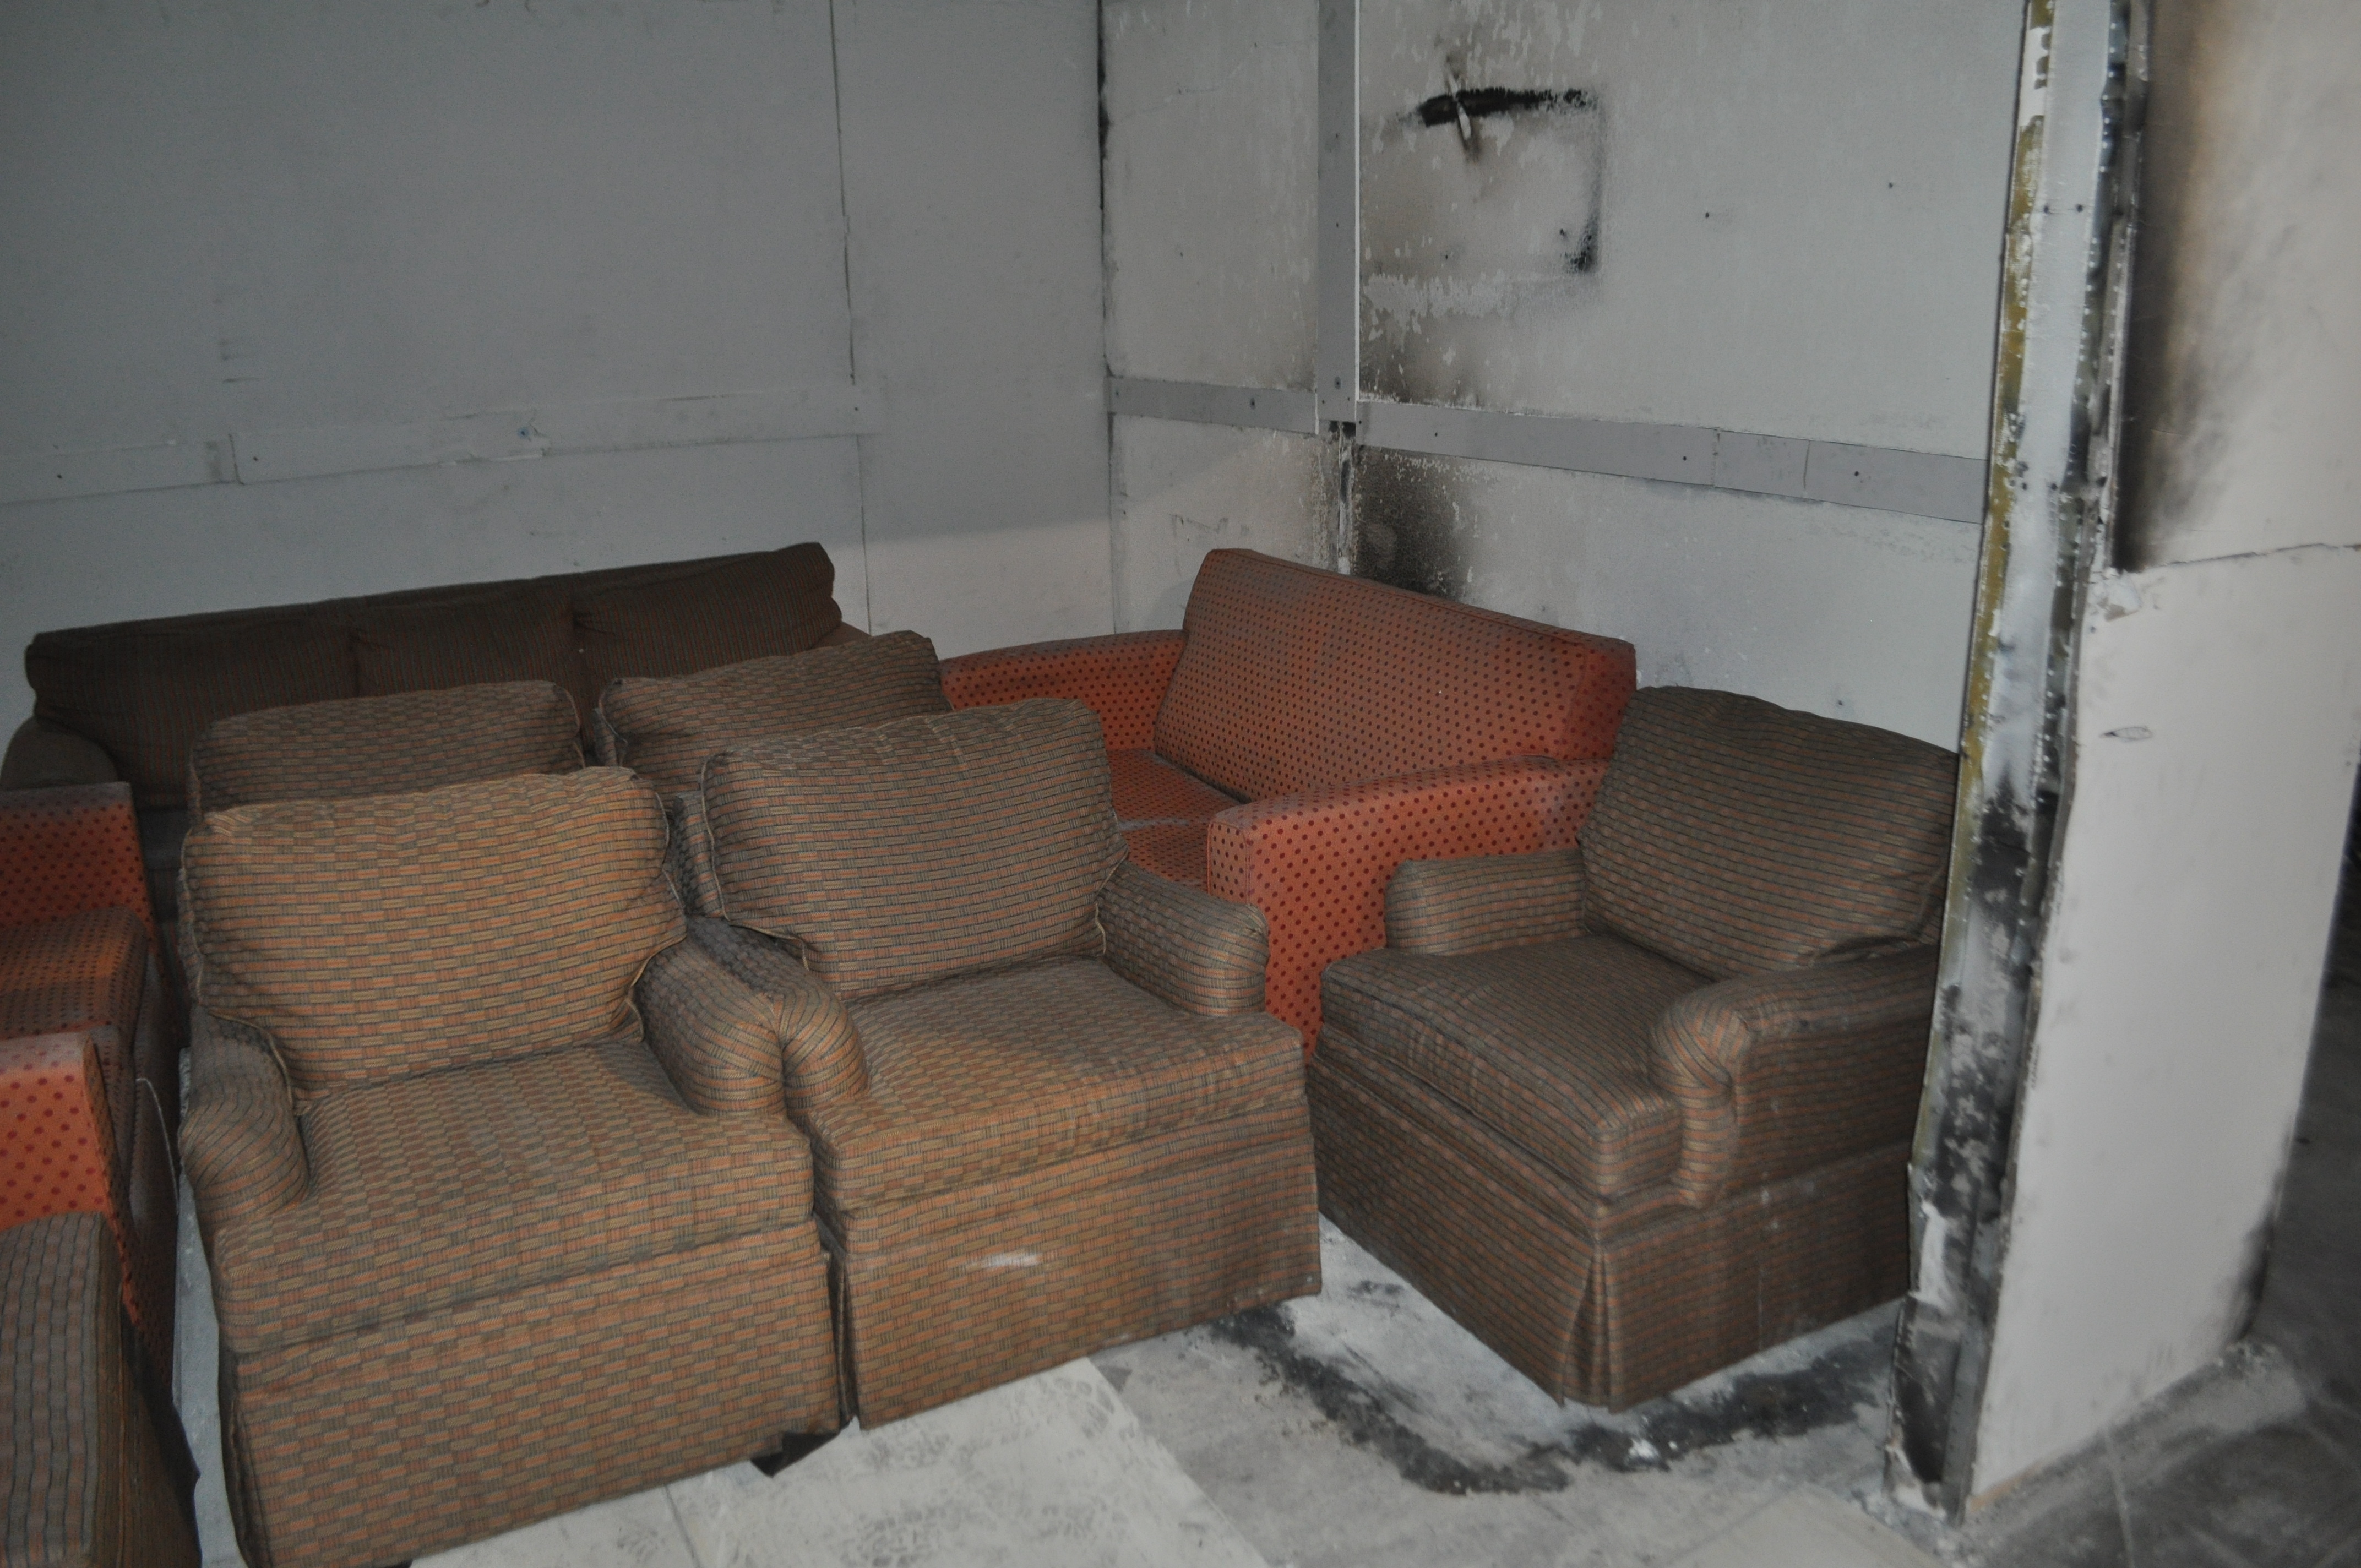
\includegraphics[width=5cm]{0_Images/Vent_Limited_Room/Horder3.jpg}} \\
	\end{tabular}
	\caption{Over Furnished Compartment}
	\label{fig:horder_images}
\end{figure}

\paragraph{Ventilation Limited Room Experiment Results} \mbox{}

In each of the compartment experiments the total heat release rate versus time was recorded using the oxygen consumption calorimeter. Although the compartment geometry was identical, the fuel load was significantly different, leading to two very different growth rates. As seen in Table \ref{table:comp_burn_results}, the furnished room reached its fully developed heat release rate at 2 minutes and 56 seconds where the overfurnished room took longer to grow, reaching its fully developed stage at 5 minutes and 46 seconds. The fully developed stage for both rooms was approximately 6500kW, until the failure of the ceiling in the overfurnished compartment failed, increasing the available oxygen, and thus the the heat release rate as seen in Figure \ref{fig:comp_burn_chart}. 

\begin{figure}[H]
	\centering
	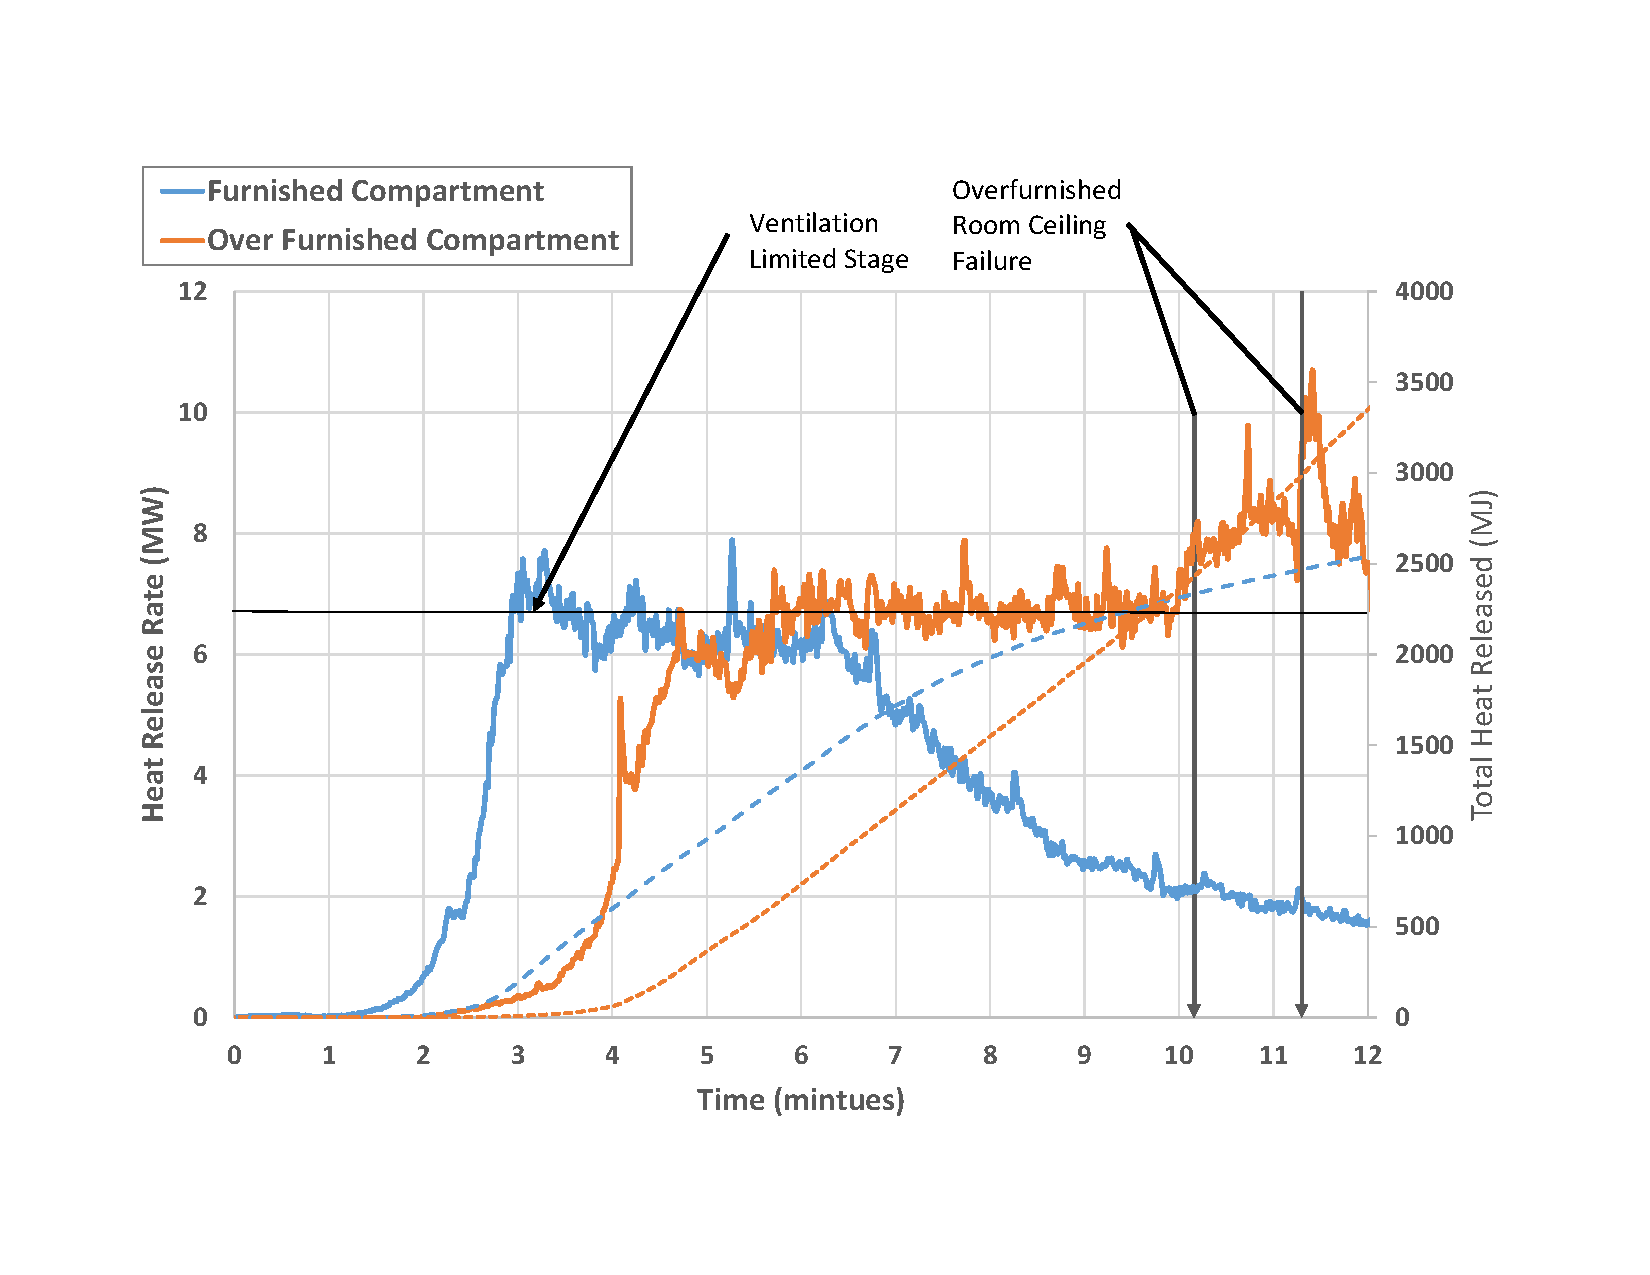
\includegraphics[width=\textwidth]{0_Images/Vent_Limited_Room/Compartment_Burn_Chart.pdf}
	\caption{Compartment Burn Results}
	\label{fig:comp_burn_chart}
\end{figure}

The difference in the two experiments was the fuel configuration, which resulted in different growh rates (Figure \ref{fig:comp_burn_chart}) The furnished compartment reached a fully developed stage within 3 minutes of ignition and maintained that heat release rate for 3 minutes before it began to decay at 6 minutes. The overfurnished compartment reached a similar peak heat release rate at just under 6 minutes and maintained that through the failure of the ceiling at 10 minutes, at which time it increased. The overfurnished compartment had more fuel to consume, thus, it remained fully developed much longer than the furnished compartment. 

Since both experiments exhibited the same peak heat release rate, the difference was the total energy that was released. The furnished compartment had a total energy release of approximately 2500MJ, where the total energy release for the over furnished compartment was approximately 3500MJ and it had yet to enter a fuel limited decay stage. The furnished compartment had entered its fuel limited decay stage however in the over furnished compartment there was still a substantial amount of fuel remaining at the time of ceiling failure. 

This demonstrates how the heat release rate or energy release rate in a compartment fire is limited by the available oxygen for combustion. The opening of the compartment served as the only means of supplying the fire with oxygen and limited its energy release. Additional fuel did not necessarily mean additional energy release per unit time. It did however, mean additional energy release over the duration of the fire. 


\begin{table}[H]
	\caption{Compartment Burn Results}
	\begin{tabular}{|c|c|c|}
		\hline
		\textbf{Experiment} & \textbf{Time to Fully Developed} & \textbf{Average Fully Developed HRR (kW)} \\ \hline \hline
		Furnished Room & 02:56 & 6458 \\ \hline
		Over Furnished Room & 05:46 & 6779 \\ \hline
	\end{tabular}
	\label{table:comp_burn_results}
\end{table}

\section{Test Structures}

\subsection{Single Story Structure} 

The house was designed by a residential architectural company to be representative of a home constructed in the mid-twentieth century with walls and doorways separating all of the rooms and 8 ft. ceilings. The experiments aim to examine the fire dynamics in a structure of this type and to further understand the impact of positive pressure attack on tenability throughout the structure.

The one-story house had an area of 1200 $ft^2$, with 3 bedrooms, 1 bathroom and 8 total rooms (Figure \ref{fig:SingleStory}). The home was a wood frame, type 5 structure lined with two layers of gypsum board (Base layer 5/8 in, Surface layer 1/2 in.) The intent of the study was to focus on content fires thus no roof structure was included in the design. The ceilings were supported with engineered i-joists instead of engineered trusses. The front and rear of the structure were covered with cement board to limit exterior fire spread. Figure \ref{fig:SingleStoryISO} is a 3D rendering of the house with the roof cut away to show the interior layout with furniture and floor coverings. The tan floor shows the carpet placement and the grey show the cement floor or simulated tile locations.

\begin{figure}[H]
	\centering
	\begin{tabular}{*2c}
		\subfloat[Single Story Side A]{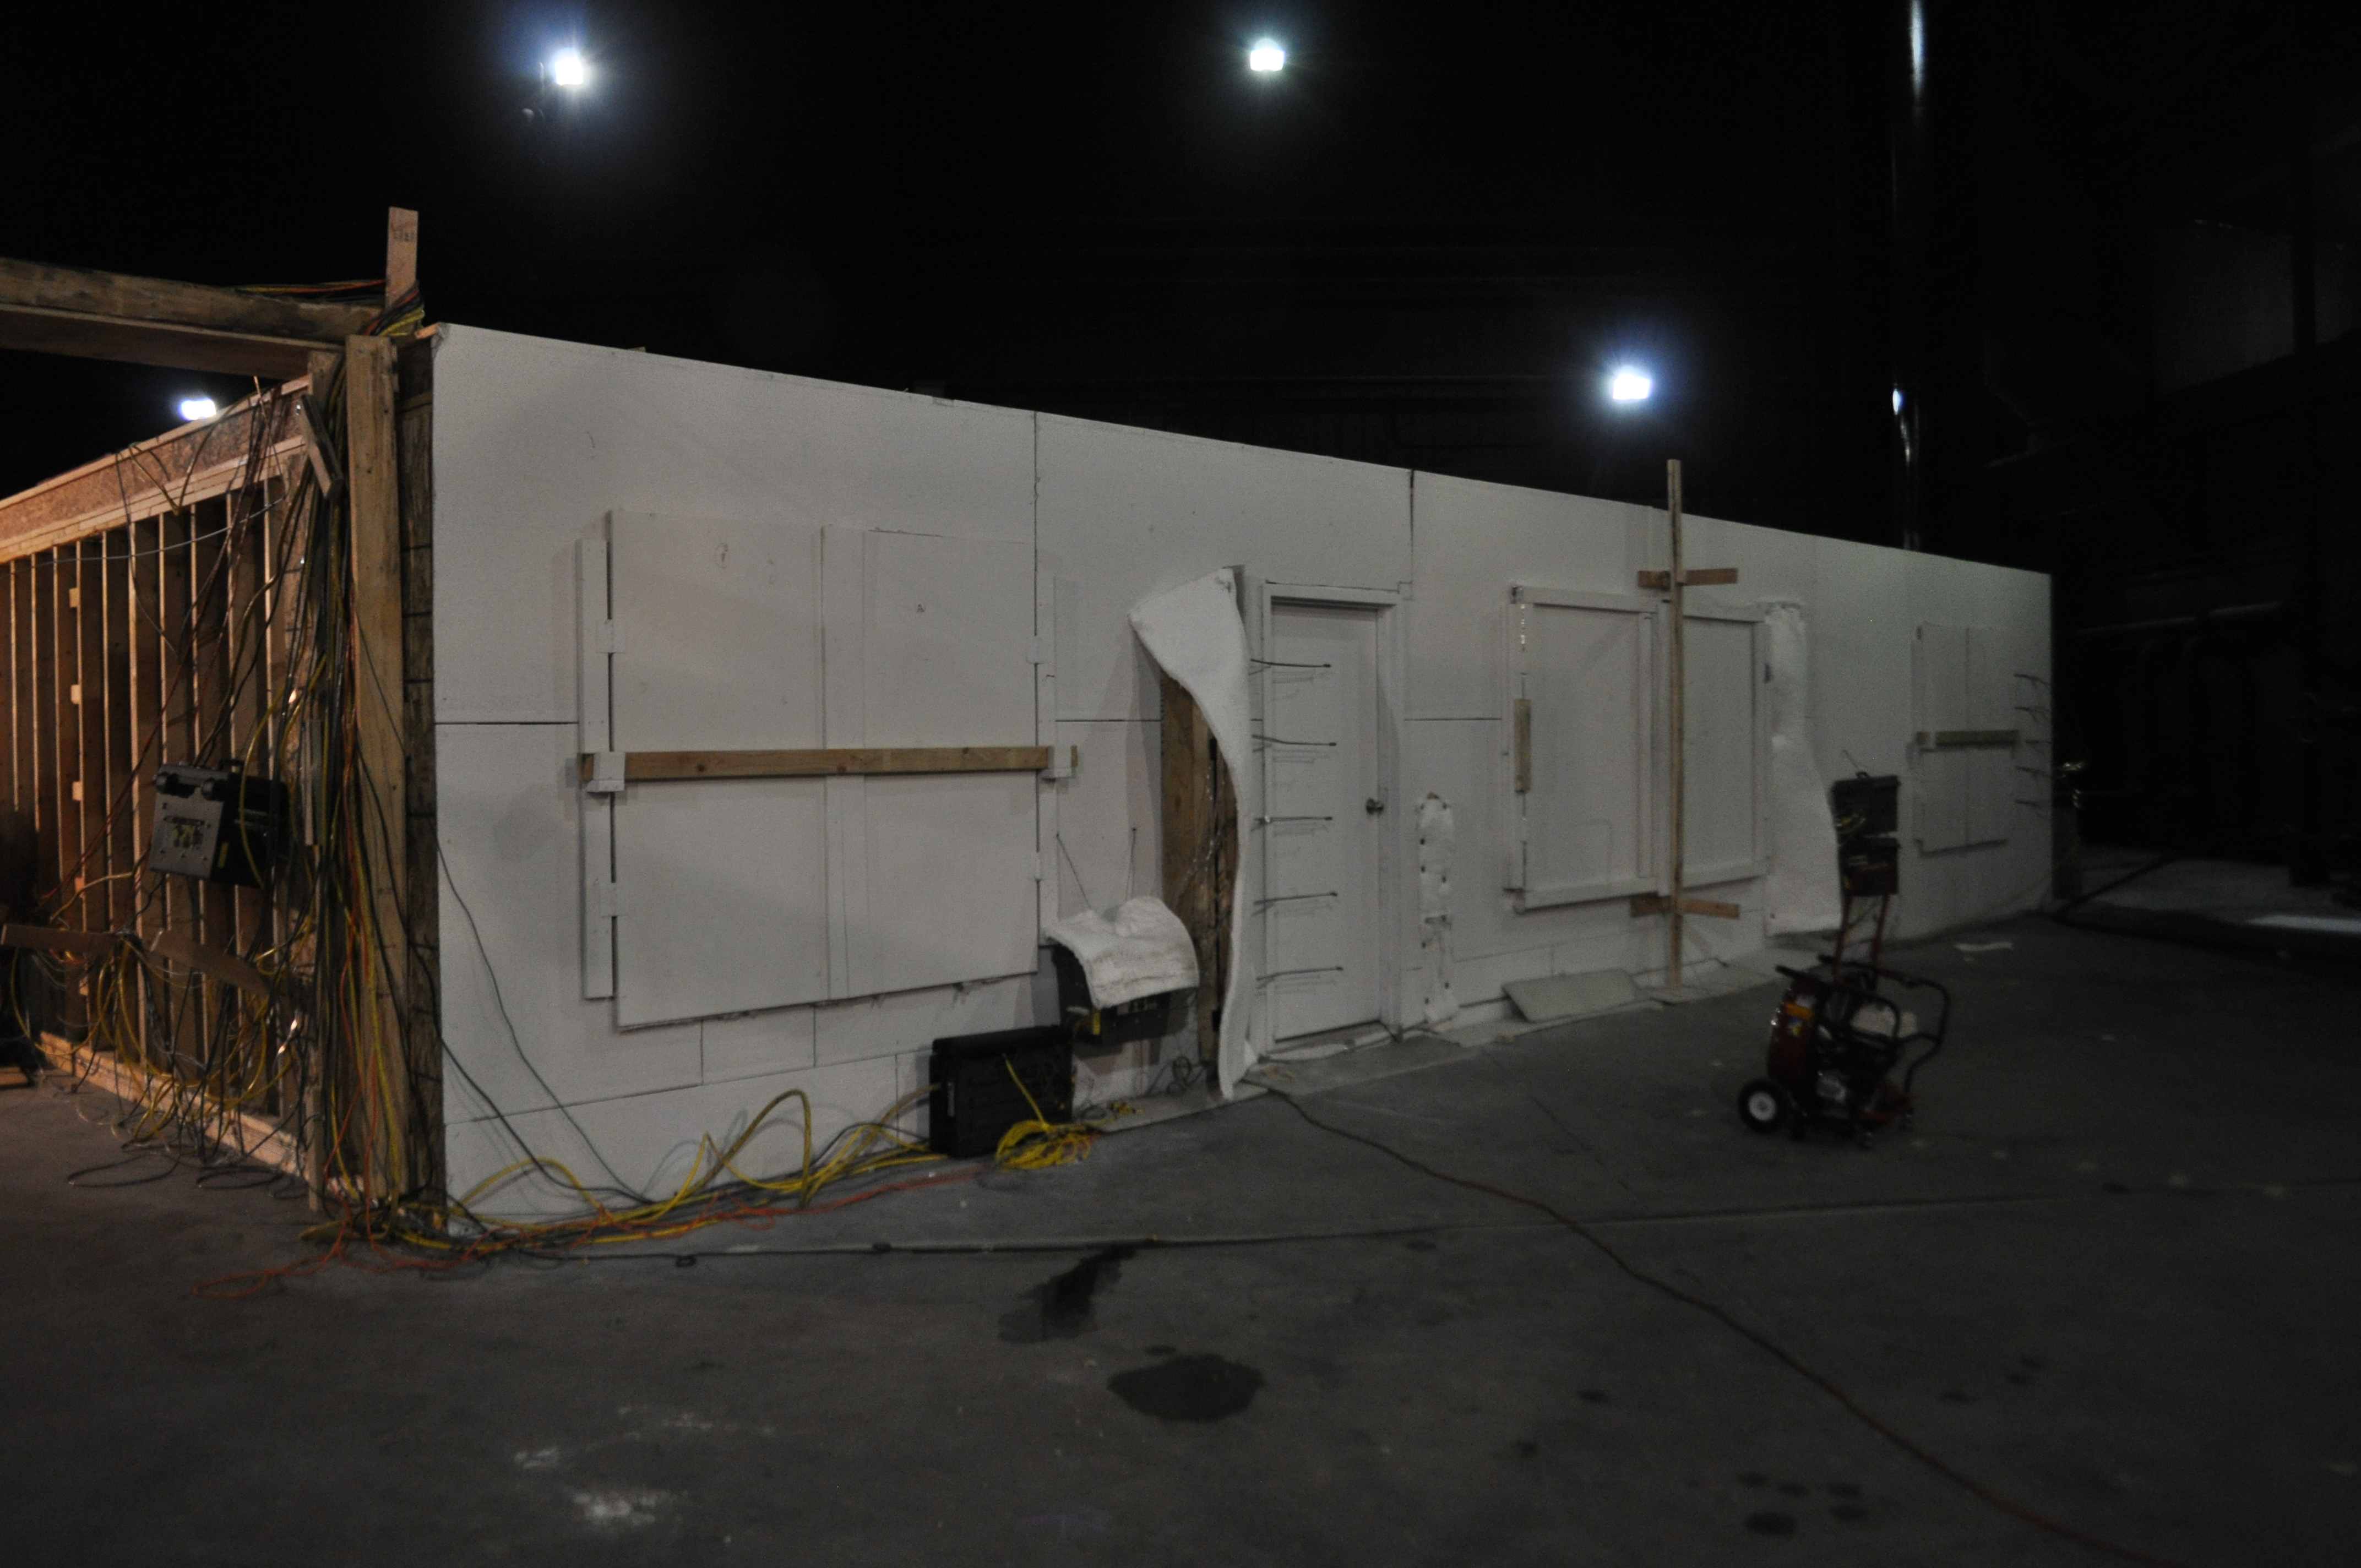
\includegraphics[width = 3in]{0_Images/Structures/SingleStory/ExteriorAB_Corner.jpg}} & 
		\subfloat[Single Story Side C]{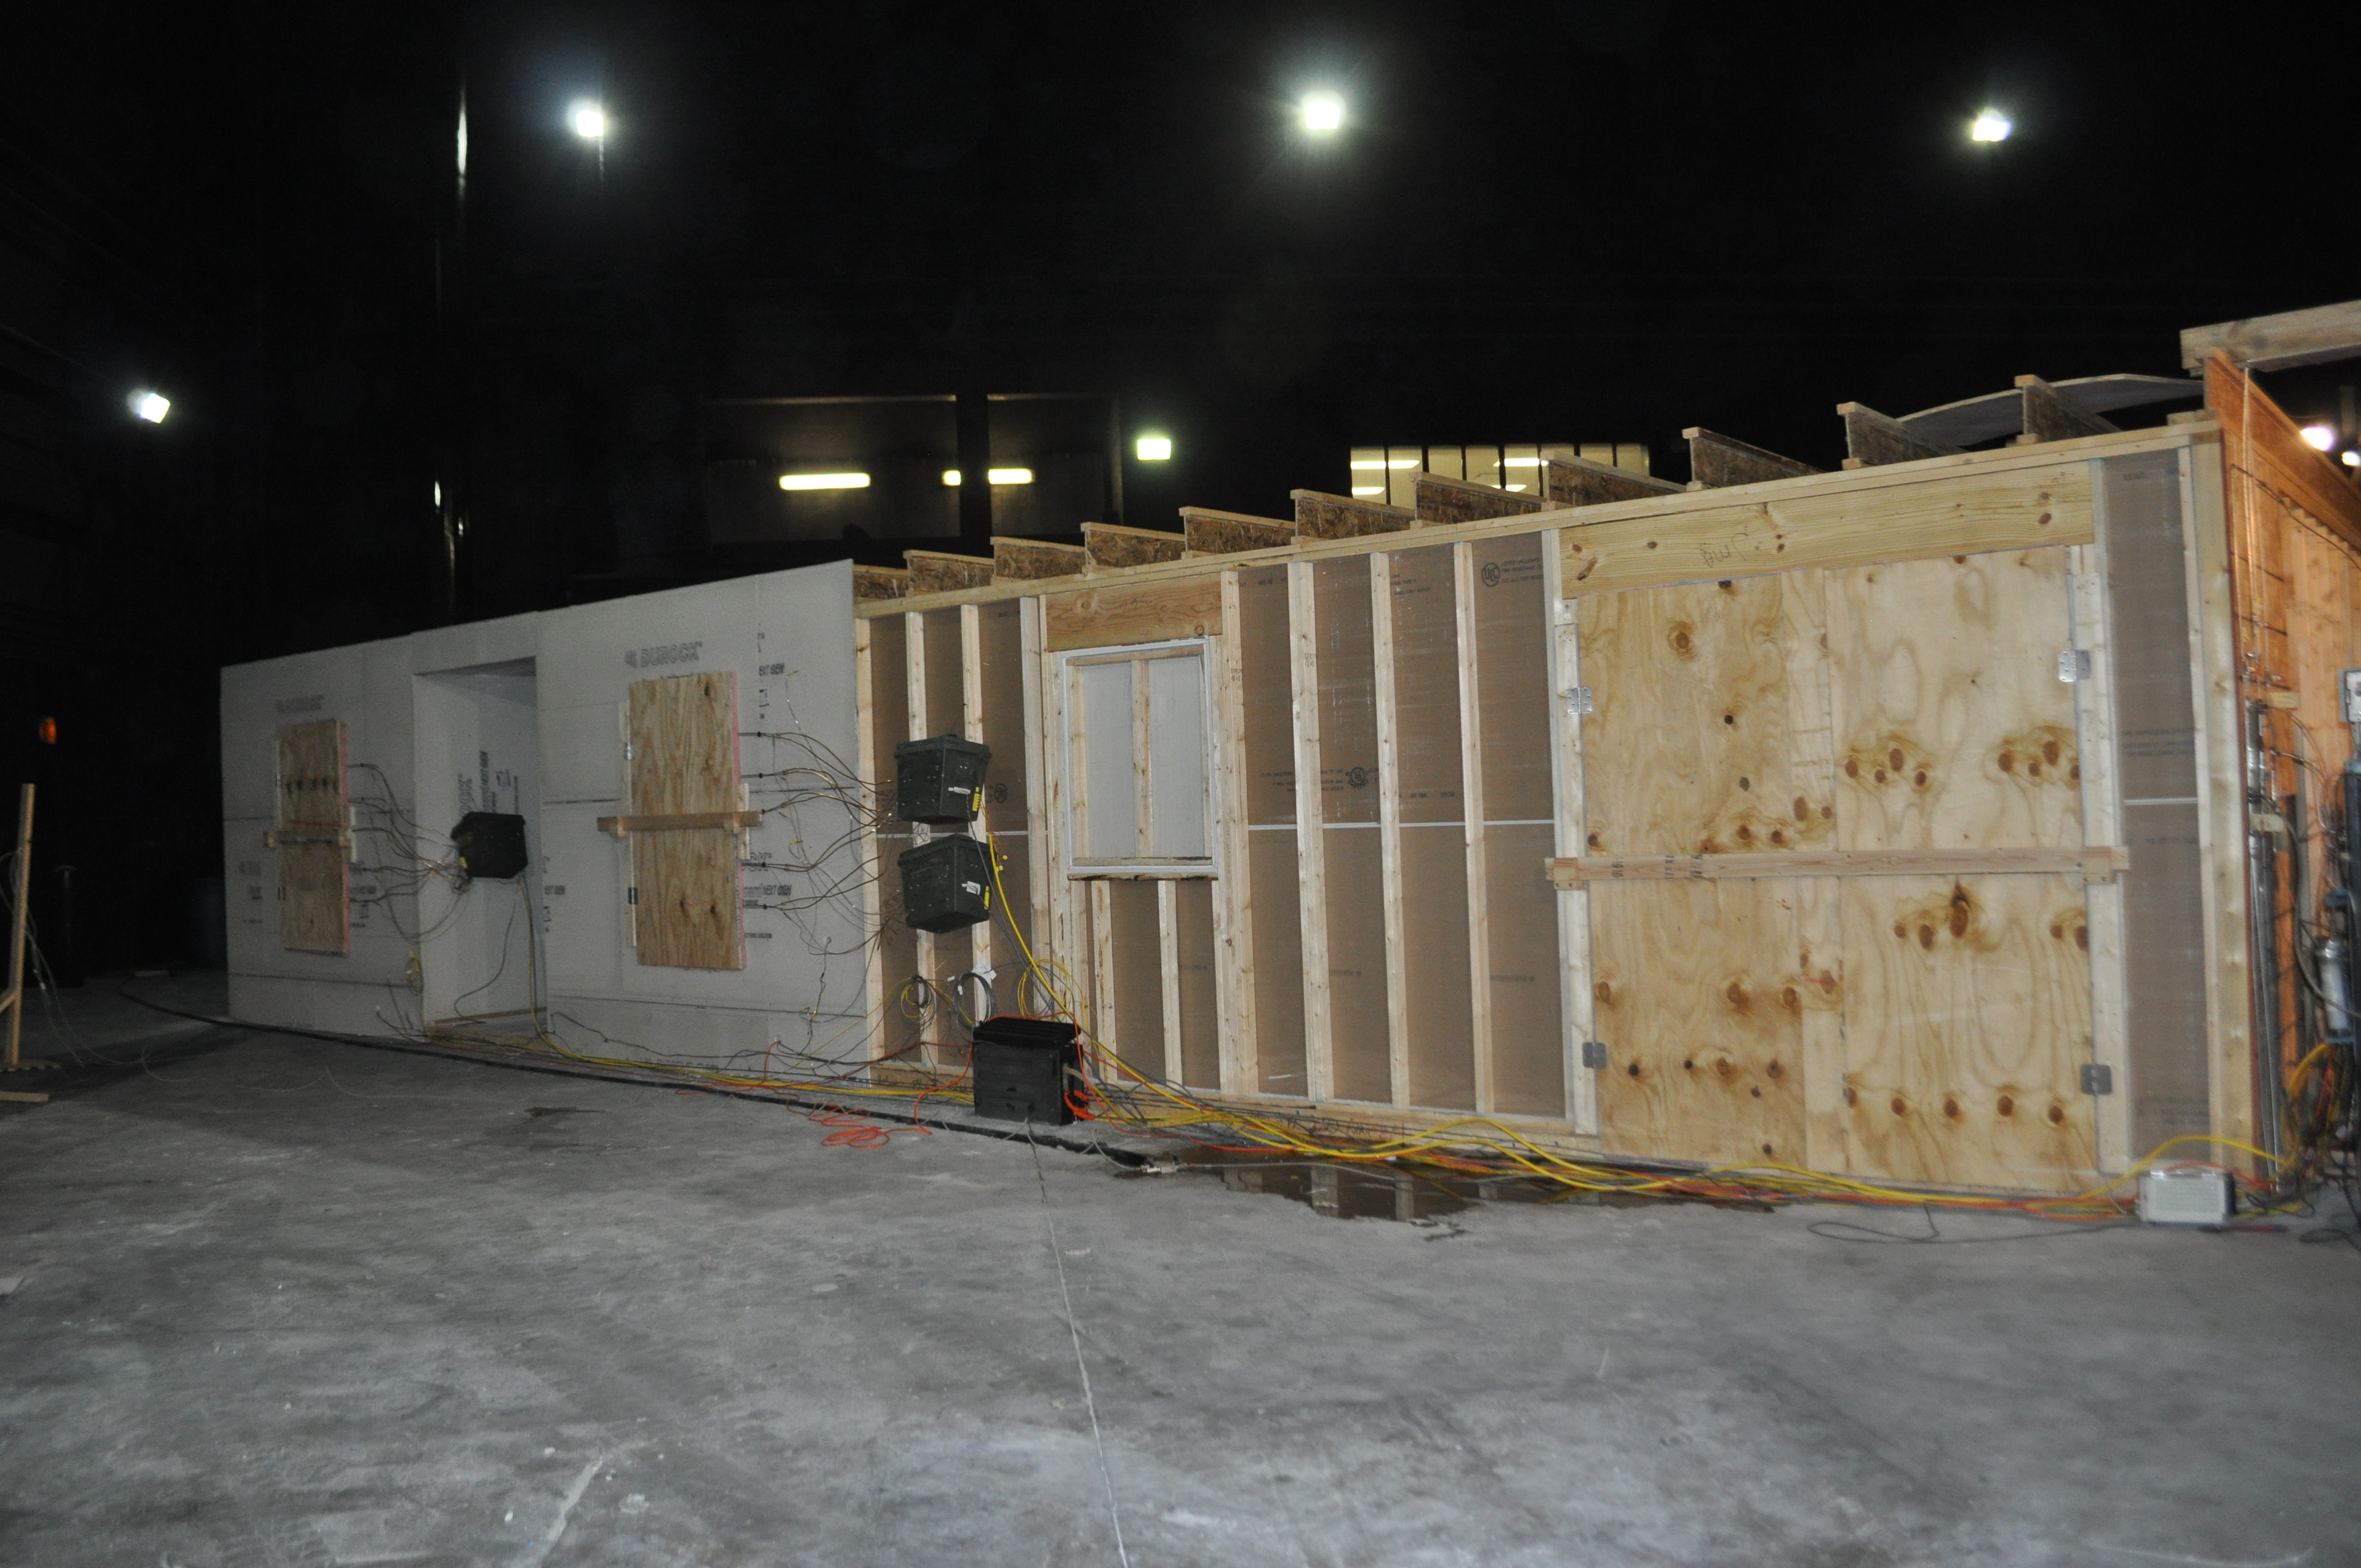
\includegraphics[width = 3in]{0_Images/Structures/SingleStory/ExteriorBC_Corner.jpg}} \\
	\end{tabular}
	\caption{Single Story Test Structure}
	\label{fig:SingleStory}
\end{figure}

\begin{figure}[H]
	\centering
	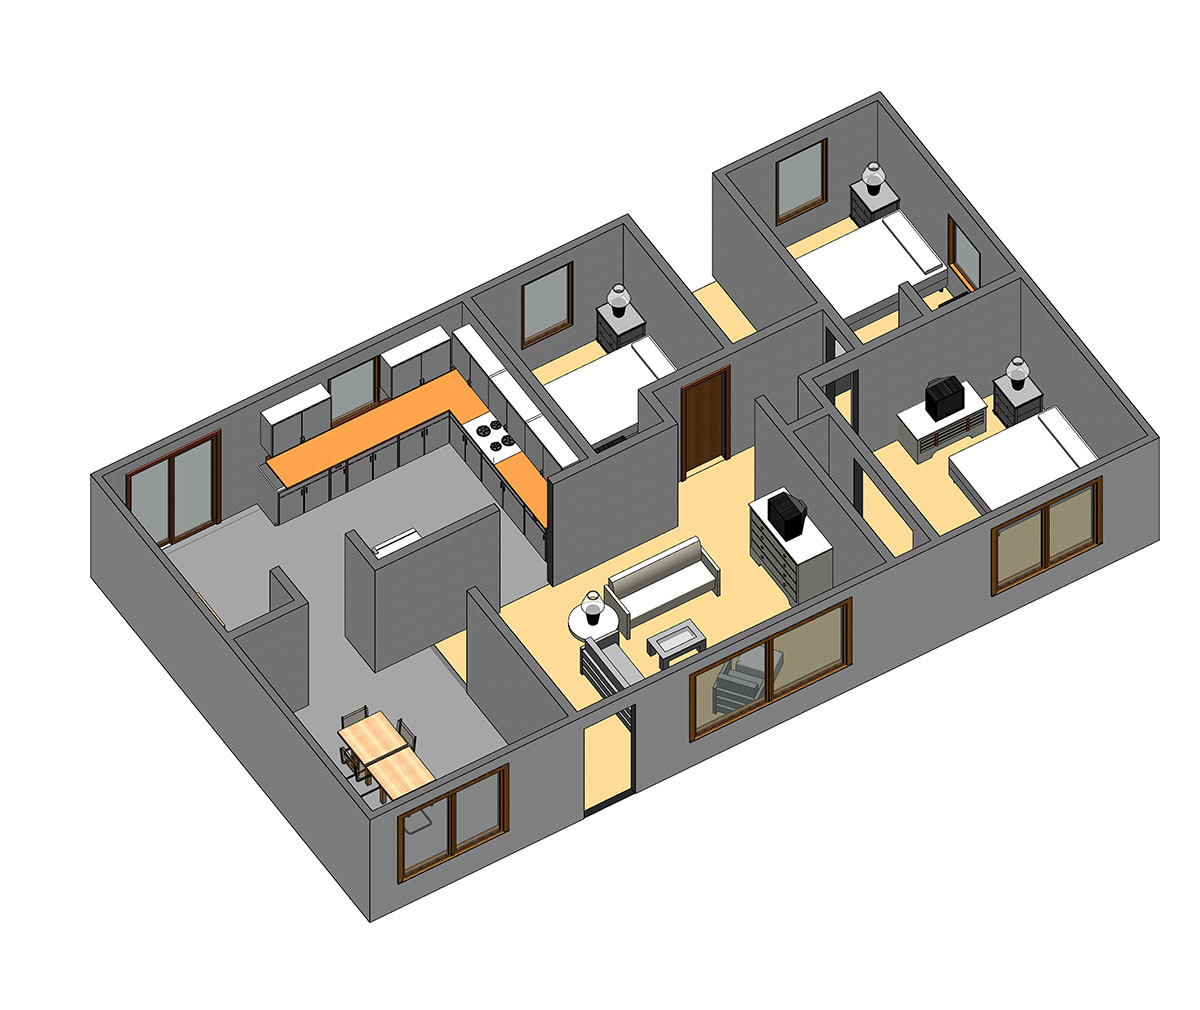
\includegraphics[width = 4in]{0_Images/Experiment_ISO/Single_Story_Base_Bed3_Closed.jpg}
	\caption{Single Story Isometric}
	\label{fig:SingleStoryISO}
\end{figure}

\subsection{Two Story Structure} 

The house was designed by a residential architectural company to be representative of a home constructed in the late-twentieth to early twenty-first century, with an open floor plan, two story foyer, and two story great room. The experiments aim to examine the fire dynamics in a structure of this type and to further understand the impact of positive pressure attack on tenability throughout the structure.

The two-story house had an area of 3200 $ft^2$, with 4 bedrooms, 2.5 bathrooms, and 12 total rooms (Figure \ref{fig:TwoStory}). This home was also a wood frame, type 5 structure lined with two layers of gypsum board (Base layer 5/8 in, Surface layer 1/2 in.) The intent of the study was to focus on content fires, thus, no roof structure was included in the design. The second floor ceilings were supported with engineered i-joists instead of engineered trusses. The front and rear of the structure were covered with cement board to limit exterior fire spread. Figure \ref{fig:TwoStoryISO} is a 3D rendering of the house with the roof cut away to show the interior layout with furniture and floor coverings. The tan floor shows the carpet placement and the grey floor shows the cement floor or simulated tile locations.

\begin{figure}[H]
	\centering
	\begin{tabular}{*2c}
		\subfloat[Two Story Side A]{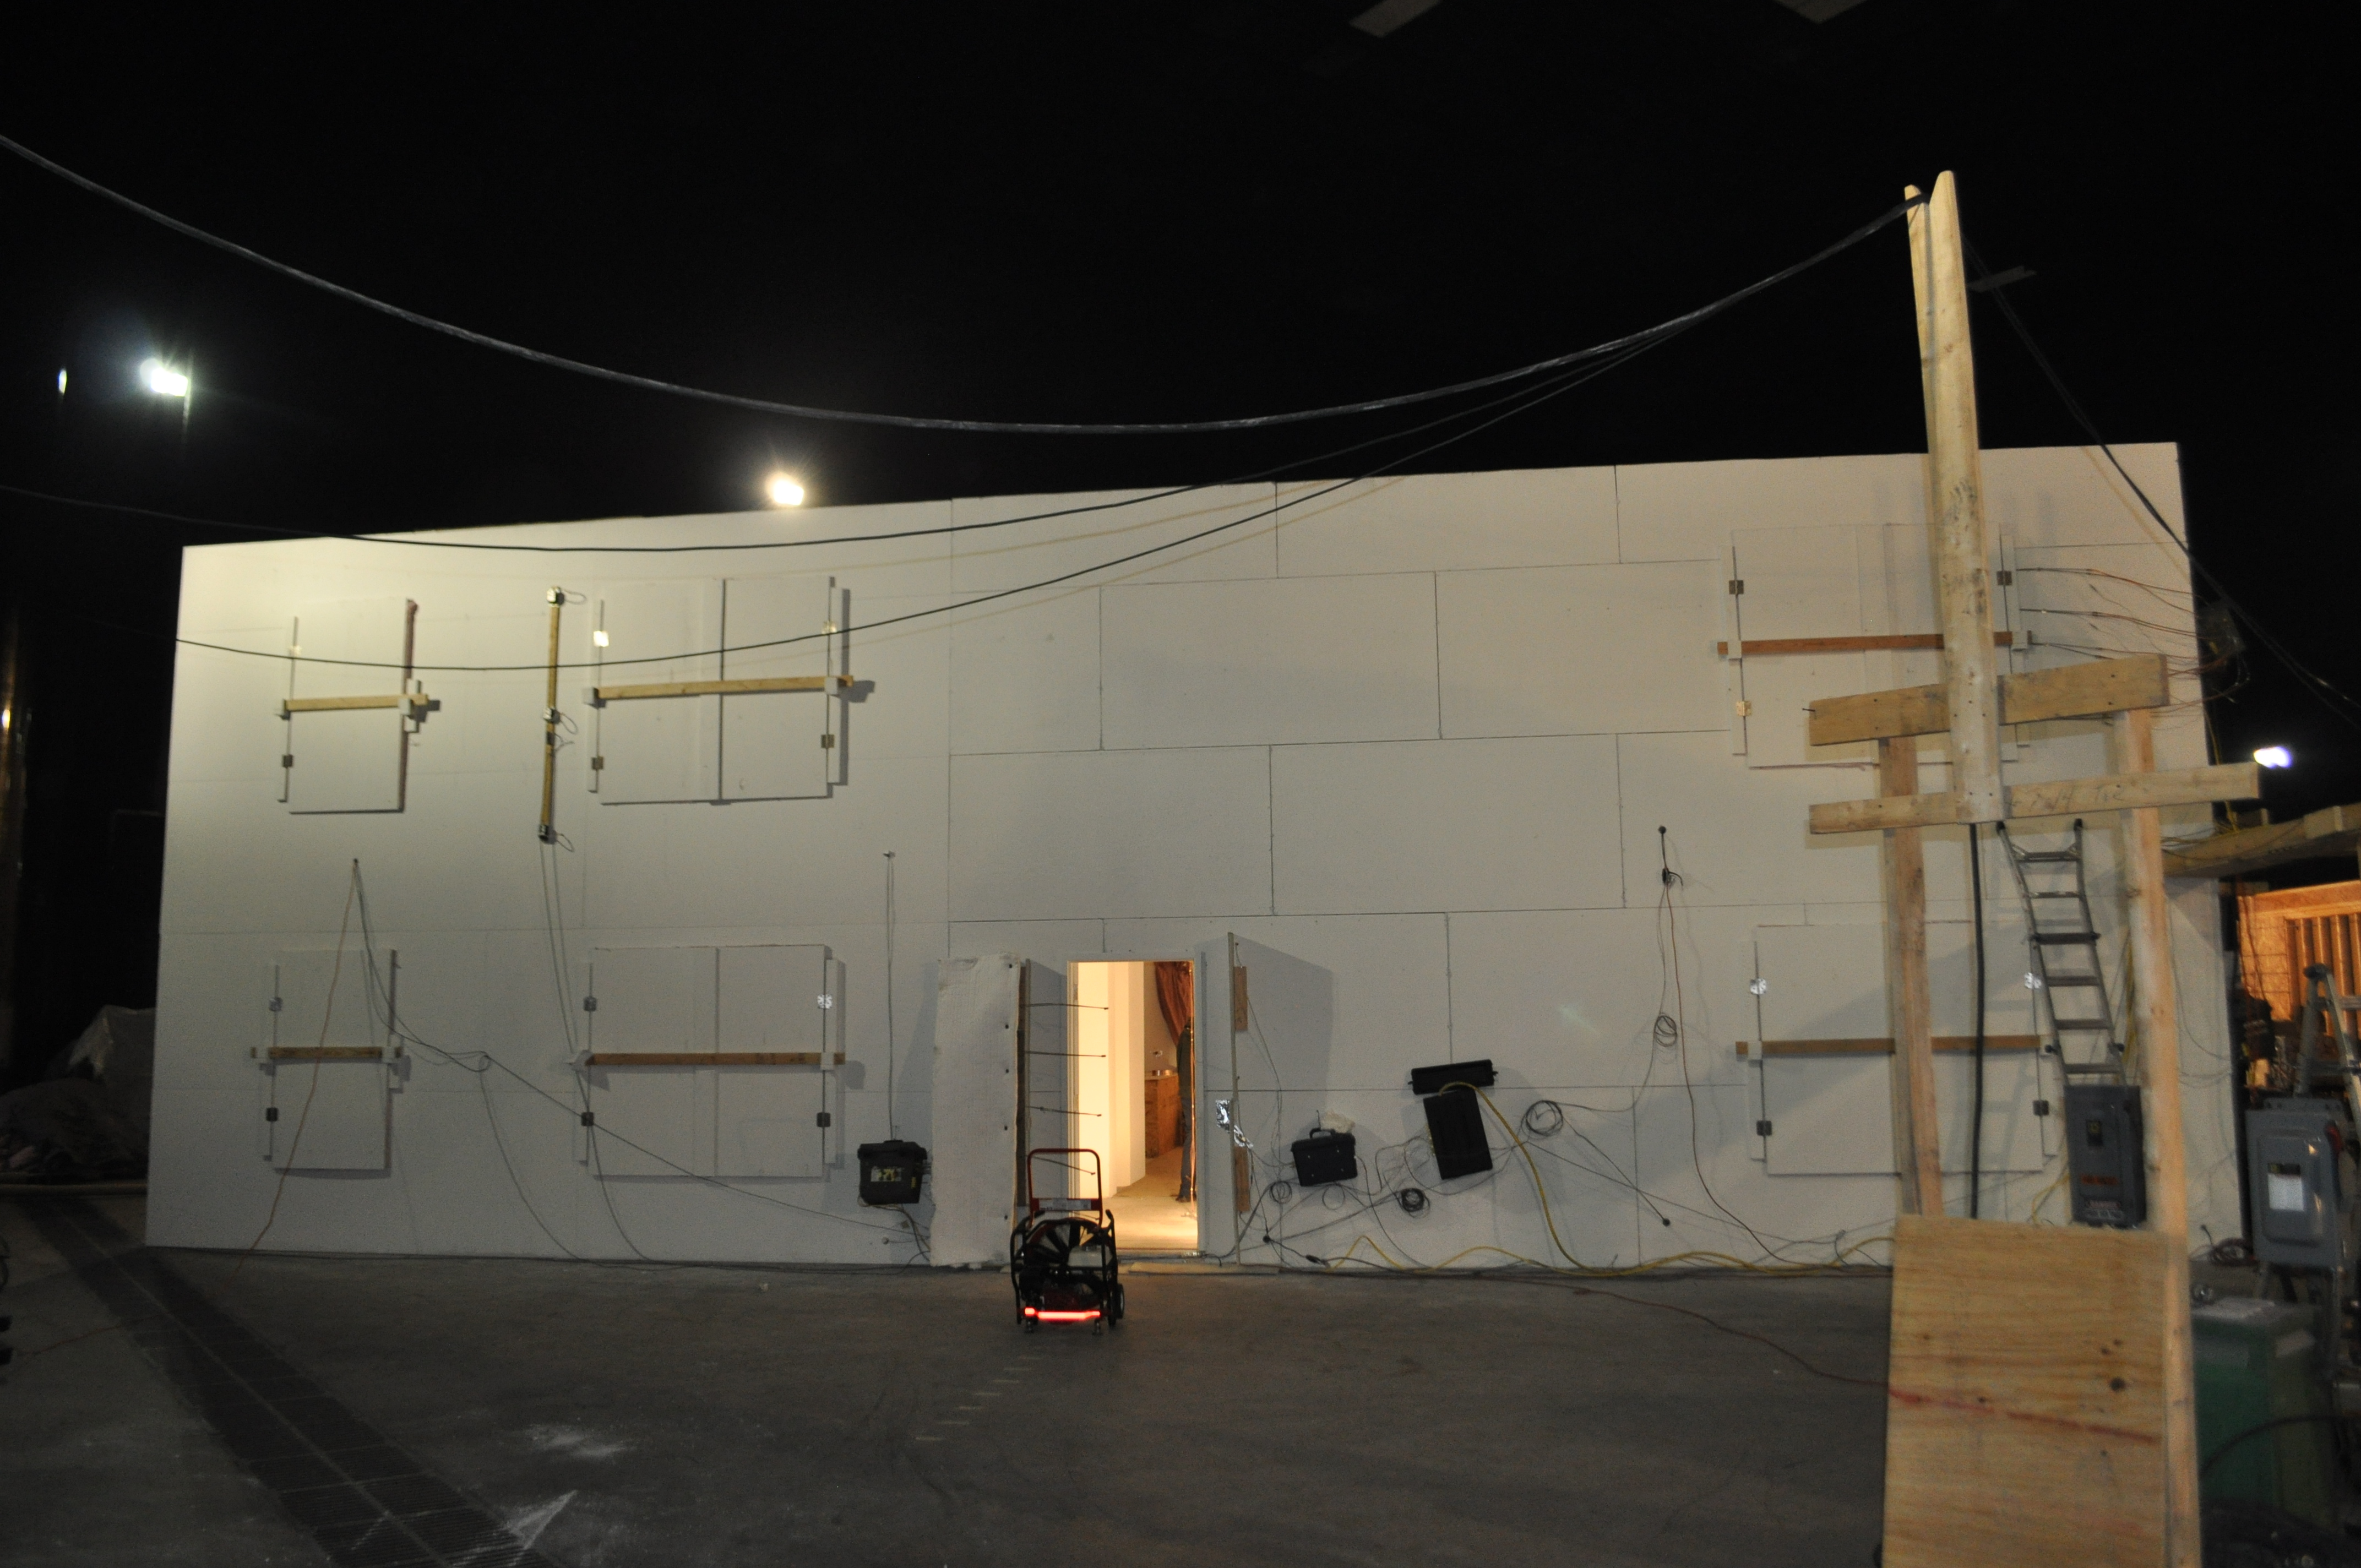
\includegraphics[width = 3in]{0_Images/Structures/TwoStory/ExteriorTwoStory_A.jpg}} & 
		\subfloat[Two Story Side C]{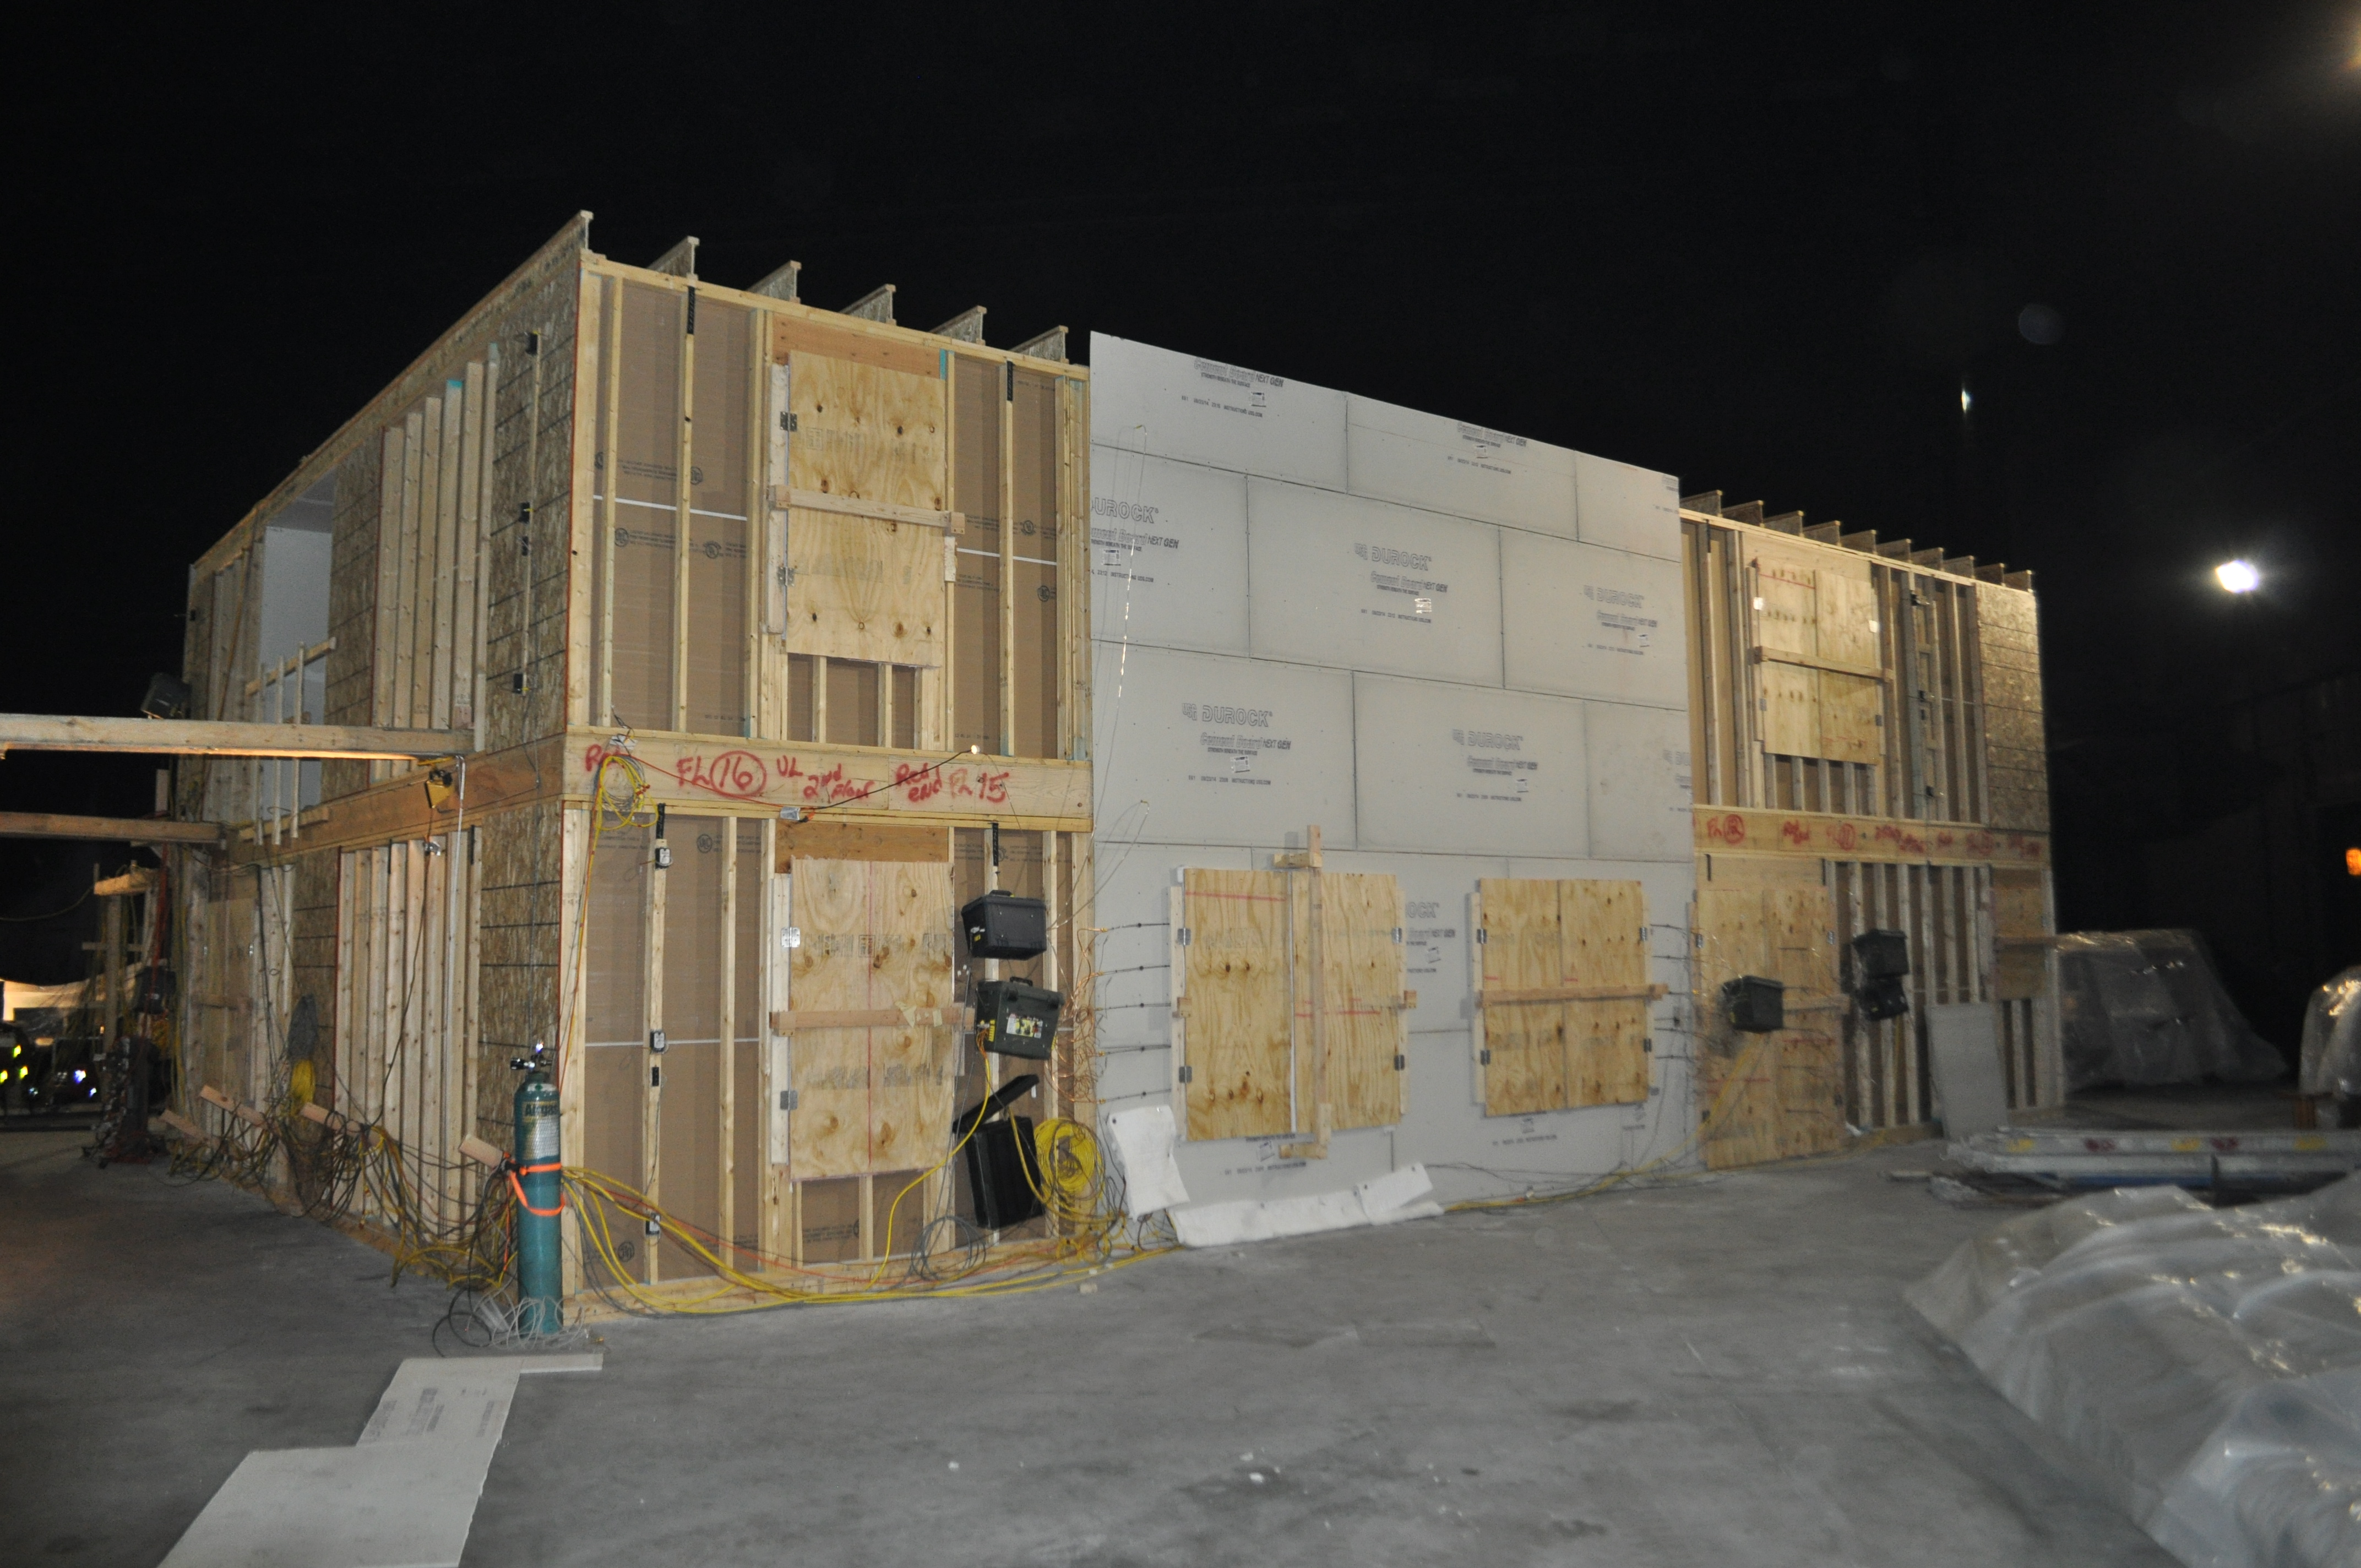
\includegraphics[width = 3in]{0_Images/Structures/TwoStory/ExteriorTwoStory_C.jpg}} \\
	\end{tabular}
	\caption{Two Story Test Structure}
	\label{fig:TwoStory}
\end{figure}

\begin{figure}[H]
	\centering
	\begin{tabular}{*2c}
		\subfloat[First FLoow]{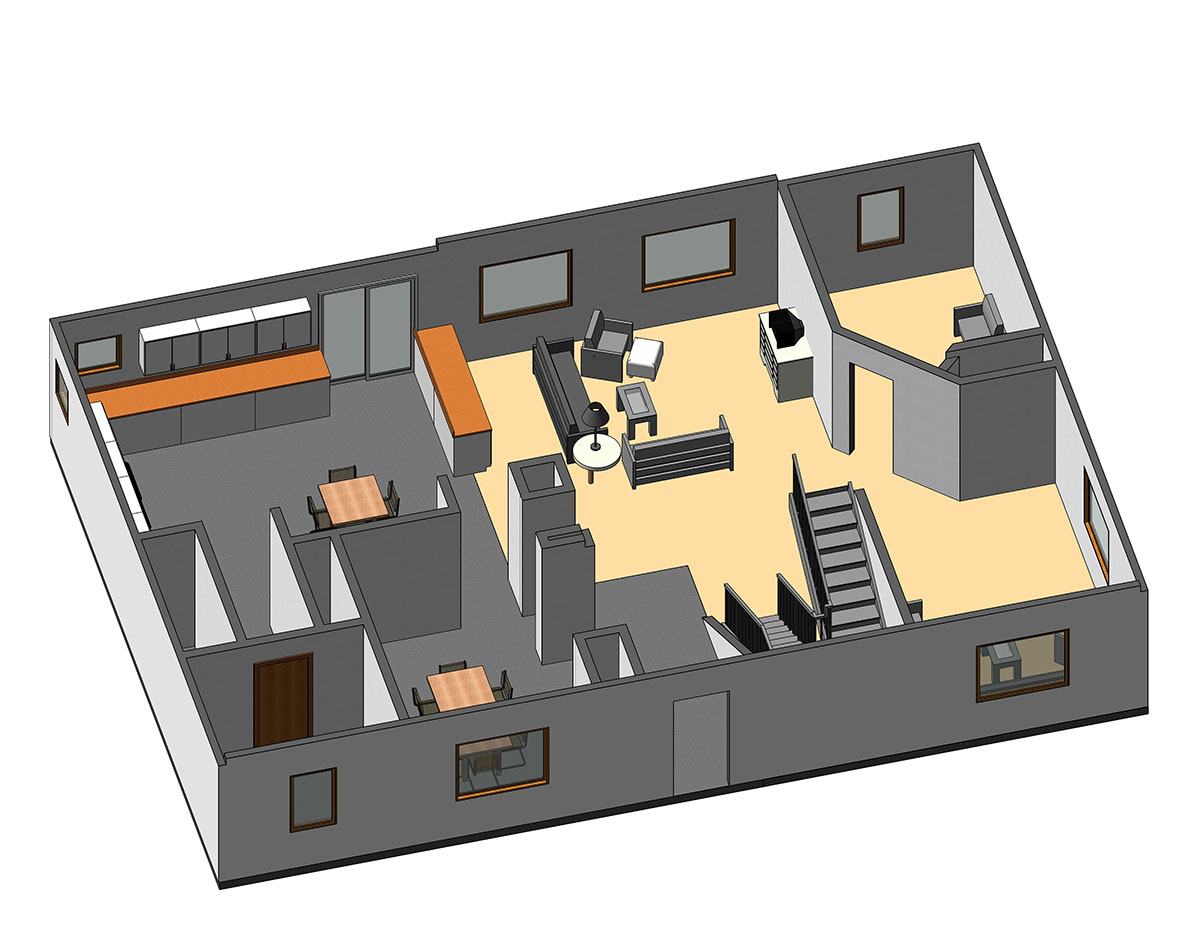
\includegraphics[width = 3in]{0_Images/Experiment_ISO/Two_Story_Base_First.jpg}} &
		\subfloat[Second Floor]{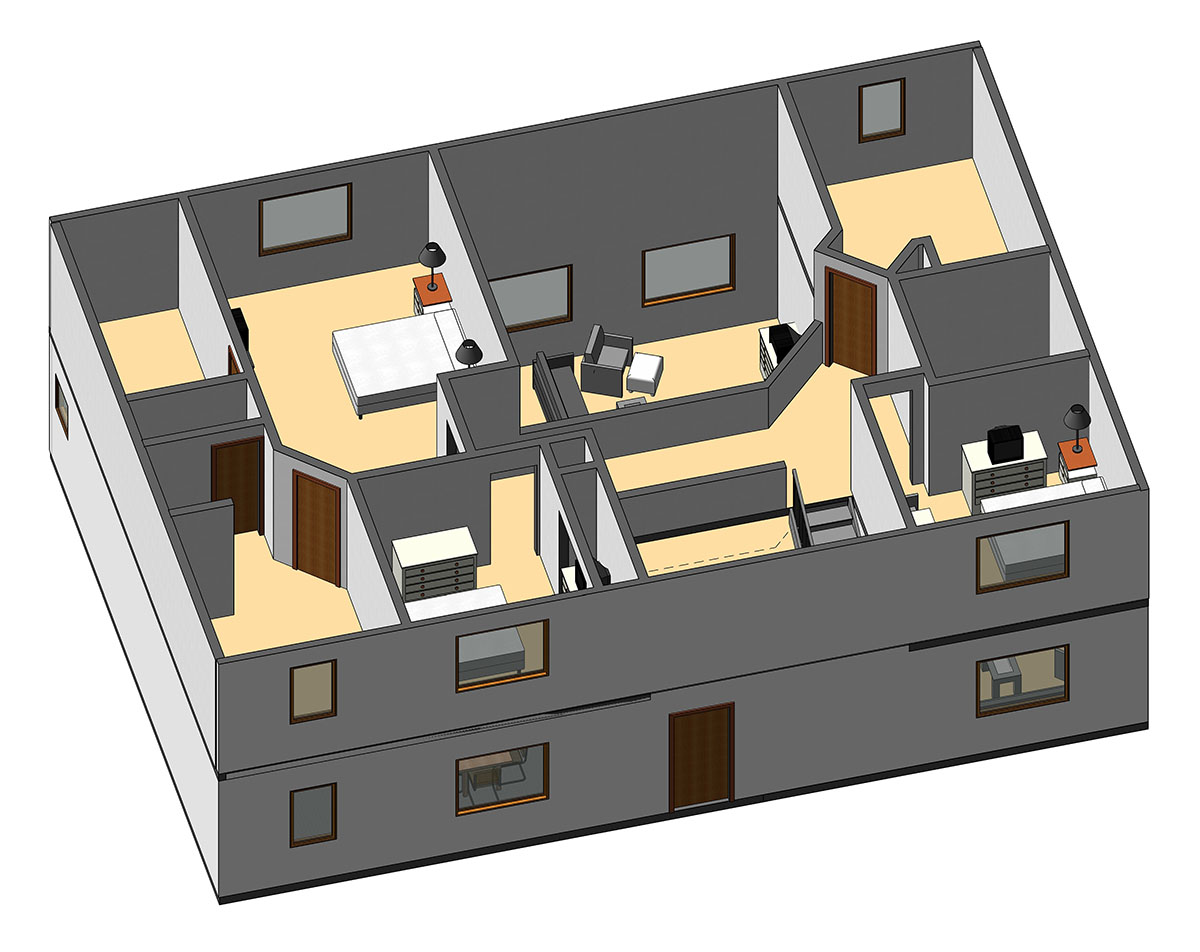
\includegraphics[width = 3in]{0_Images/Experiment_ISO/Two_Story_Base_Second.jpg}} \\
	\end{tabular}
	\caption{Two Story Isometric}
	\label{fig:TwoStoryISO}
\end{figure}

\section{Cold Flow Experiments}
Prior to conducting full scale fire tests, cold flow tests were conducted to establish a baseline of how positive pressure fans affect the airflow in residential structures. The results of the cold flow experiments were used by the project technical panel to select a single fan to be for use in the full scale fire experiments. A total of 24 experiments were run using six different fans provided by Leader, RamFan, SuperVac, Tempest, UniFire and Ventry. Each manufacturer graciously provided the use of one 18" gas and the comparable 18" electric fan. Table \ref{table:cold_flow_Fans} shows the fans tested, manufacturer and model number. 

\begin{table}[H]
	\centering
	\caption{Fans Used in Cold Flow Experiments}
	\begin{tabular}{|c|c|c|}
		\hline
		Manufacturer & Drive Method (Electric or Gas) & Model Number \\ \hline \hline
		Leader & Gas & MT236 \\ \hline
		Leader & Electric & EDS 230 \\ \hline
		Ramfan & Gas & GX350 \\ \hline
		Ramfan & Electric & EX500 \\ \hline
		Super Vac & Gas & 718G4-H \\ \hline
		Super Vac & Electric & 718VR3 \\ \hline
		Tempest & Gas & BD-18-H-5.5 \\ \hline
		Tempest & Electric & VS-18-R-2.0 \\ \hline
		Unifire & Gas & DST-3P4 \\ \hline
		Unifire & Electric & EB18SP \\ \hline
		Ventry & Gas & 20GX160 \\ \hline
		Ventry & Electric & 20E1.5GFCI \\ \hline
	\end{tabular}
	\label{table:cold_flow_Fans}
\end{table}

This report is not intended to identify the pros and cons of a particular fan or manufacturer. Thus, cold flow results will be presented in a generic fashion leaving the identifying characteristics of the fans out of the results. 

To control the number of variables within the full scale testing, it was necessary to select a single fan for use in all fire tests. It was identified through a poll of our technical panel and an online survey of our social media followers that the majority of the organizations using PPA were utilizing a gas fan. The specific gas fan was selected by the technical panel after evaluating the cold flow data with a ratio of 1:1 in the single story and 2:1 in the two story. The panel decided on the use of the average fan based on flow rate through the exhaust opening.

\section{Full Scale Fire Experiments}

\subsection{Single Story Experiments} \label{SingleStoryExp}

Fifteen full scale fire experiments were conducted in the single story 1200$ft^2$ ranch style structure. Experiments were intended to test the impact of PPA on fire dynamics in a compartmented single story structure. Variables within the experiments were the ignition location, fan positioning and exhaust size and location. Table \ref{table:SingleStoryExperiments} lists the experiment number, ignition location, fan position and exhaust for each of the experiments performed in the single story structure.

\mbox{}

\begin{table}[H]
	\centering
	\caption {Single Story Experiments}
	\begin{tabular}[c]{|c|C{5cm}|c|C{5cm}|}
		\hline
		\textbf{Experiment} & \textbf{Ignition Location} & \textbf{Fan Position} & \textbf{Exhaust} \\ \hline \hline
		1 & Living Room & Front Door & Living Room Window \\ \hline
		2 & Living Room & Front Door & Living Room Window \\ \hline
		3 & Bedroom 2 & Front Door & Bedroom 2 Windows \\ \hline
		4 & Living Room & Front Door  & Bedroom 2 Rear Window \\ \hline
		5 & Living Room & Front Door & Living Room Window \& Bedroom 2 Rear Window \\ \hline
		6 & Living Room & Front Door & Bedroom 2 Windows \\ \hline
		*7 & Bedroom 3 & Front Door & Bedroom 3 Window \\ \hline
		8 & Bedroom 2 & Front Door & Bedroom 2 Rear Window \\ \hline
		9 & Bedroom 2 & Front Door & Bedroom 2 Rear Window \\ \hline
		10 & Bedroom 2 & Front Door & Bedroom 2 Rear Window \\ \hline
		11 & Bedroom 2 & Front Door & Master Bedroom, Bedroom 2, Bedroom 3 Windows \\ \hline
		12 & Bedroom 3 & Front Door & Bedroom 2 Rear Window \\ \hline
		13 & Bedroom 3 & Front Door & Bedroom 3 Window \\ \hline
		14 & Kitchen & Front Door & Bedroom 2 Rear Window \\ \hline
		15 & Master Bedroom, Bedroom 2, Bedroom 3 & Front Door & Master Bedroom, Bedroom 2, Bedroom 3 Windows \\ \hline
	\end{tabular}
		\begin{tablenotes}
			\item *Fan Setback 15$ft$ vs standard 7$ft$
		\end{tablenotes}
	\label{table:SingleStoryExperiments}
\end{table}

\subsection{Two Story Experiments} \label{TwoStoryExp}

Ten full scale fire experiments were conducted in the two story 3200$ft^2$ ranch style structure. Experiments were intended to test the impact of PPA on fire dynamics in a open plan two story structure. Variables within the experiments were the ignition location, fan positioning and exhaust size and location. Table \ref{Tab:TwoStoryExperiments} lists the experiment number, ignition location, pan placement and exhaust location for each of the experiments preformed in the two story structure.

\begin{table}[H]
	\centering
	\caption{Two Story Experiments}
	\begin{tabular}[c]{|c|C{5cm}|c|C{5cm}|}
		\hline
		\textbf{Experiment} & \textbf{Ignition Location} & \textbf{Fan Position} & \textbf{Exhaust} \\ \hline \hline
		16 & Family Room & Front Door & Family Room Window \\ \hline
		17 & Family Room & Front Door & Family Room Window \\ \hline
		18 & Family Room & Front Door & Family Room Window \\ \hline
		19 & Family Room & Front Door & Bedroom 3 Window \\ \hline
		20 & Family Room & Front Door & Family Room 1, Family Room 2 Windows \\ \hline
		21 & Family Room & Front Door & Family Room Window \\ \hline
		22 & Family Room & Front Door & Bedroom 2 Rear Window \\ \hline
		23 & Bedroom 3 & Front Door & Bedroom 3 Window \\ \hline
		24 & Bedroom 3 & Front Door & Bedroom 3 Window, 1/2 Rear Door \\ \hline
		25 & Bedroom 4 & Front Door & Bedroom 4 Window \\ \hline
	\end{tabular}
	\label{Tab:TwoStoryExperiments}
\end{table}

\subsection{Smoke Removal Experiments}

To identify the effectiveness of systematic versus non-systematic smoke removal using positive pressure ventilation, two experiments were conducted in the 1200 $ft^2$ single story structure. A single upholstered chair was positioned in the kitchen away from other fuels. The chair was ignited via an electric match behind the top cushion. The chair was permitted to burn until the majority of the chair had burned away and temperatures had reduced to 200$^{\circ}F$. The chair was then removed, simulating extinguishment of the fire, at which time the smoke exhaust experiment was preformed. For the systematic case, the bedroom windows were opened one at at time, allowing the room to clear before proceeding to the next window. For the non-systematic case, all bedroom windows were open similaniously. 

\section{Tactical Considerations}

\subsection{Understanding the Basics of Positive Pressure}

\paragraph{Pressure} \mbox{}

Pressure in the fire service is typically thought of in the units of pounds per square inch (PSI), as this is the standard pressure unit for many of the pump panel gauges on an engine. This, however, is not the only unit for pressure. The scientific community uses the units of Pascal (Pa).  1Pa is equal to 0.00015PSI. Standard atmospheric pressure, 1 atm  is equal to 14.7 PSI or 101,325 Pa. When pressure is discussed in this report it is referring to the differential pressure ($\Delta$P), where the reference pressure is atmospheric pressure. An example of this would be the interior pressure of a house as compared to an the outside pressure. The $\Delta$P could be 5Pa where the pressure inside would be 101,330 Pa and the exterior pressure is 101,325 Pa.  

\paragraph{Fire Flows are Caused by Pressure} \mbox{}

One by-product of the combustion reaction is heat, most often thought of as ``hot gases''. The hot gases are made up of the products of combustion mixed with the air in the proximity of the fire. As these gases are heated they expand, becoming less dense. When confined in a compartment or structure, the expanding gases create pressure. When one area of a structure has a different pressure than an adjacent area a flow occurs. The greater the differential pressure, the greater the velocity of flow. Pressure always flows from high to low. This flow is the primary method of heat transfer (convection) from one compartment to the next in a structure fire. 

\paragraph{Ventilation} \mbox{}

The gases and soot produced during a fire are less dense than the density of the ambient air both inside and outside the structure. This makes them buoyant. When firefighters preform ventilation, they are using this buoyancy to their advantage. The less dense fire gases flow out of the structure. As less dense gases flow out of the structure up high, they create a lower pressure inside than outside, drawing in ambient air down low. The flows during both horizontal and vertical ventilation use the buoyancy of the gases in order to reduce temperatures, toxic gas concentrations, and given enough time, visibility if cordinated with suppression. Positive pressure ventilation seaks to alter the buoyant flows within the structure during a fire. 

\begin{figure}[H]
	\centering
	\begin{tabular}{c c }
		\subfloat[Flow with Horizontal Ventilation]{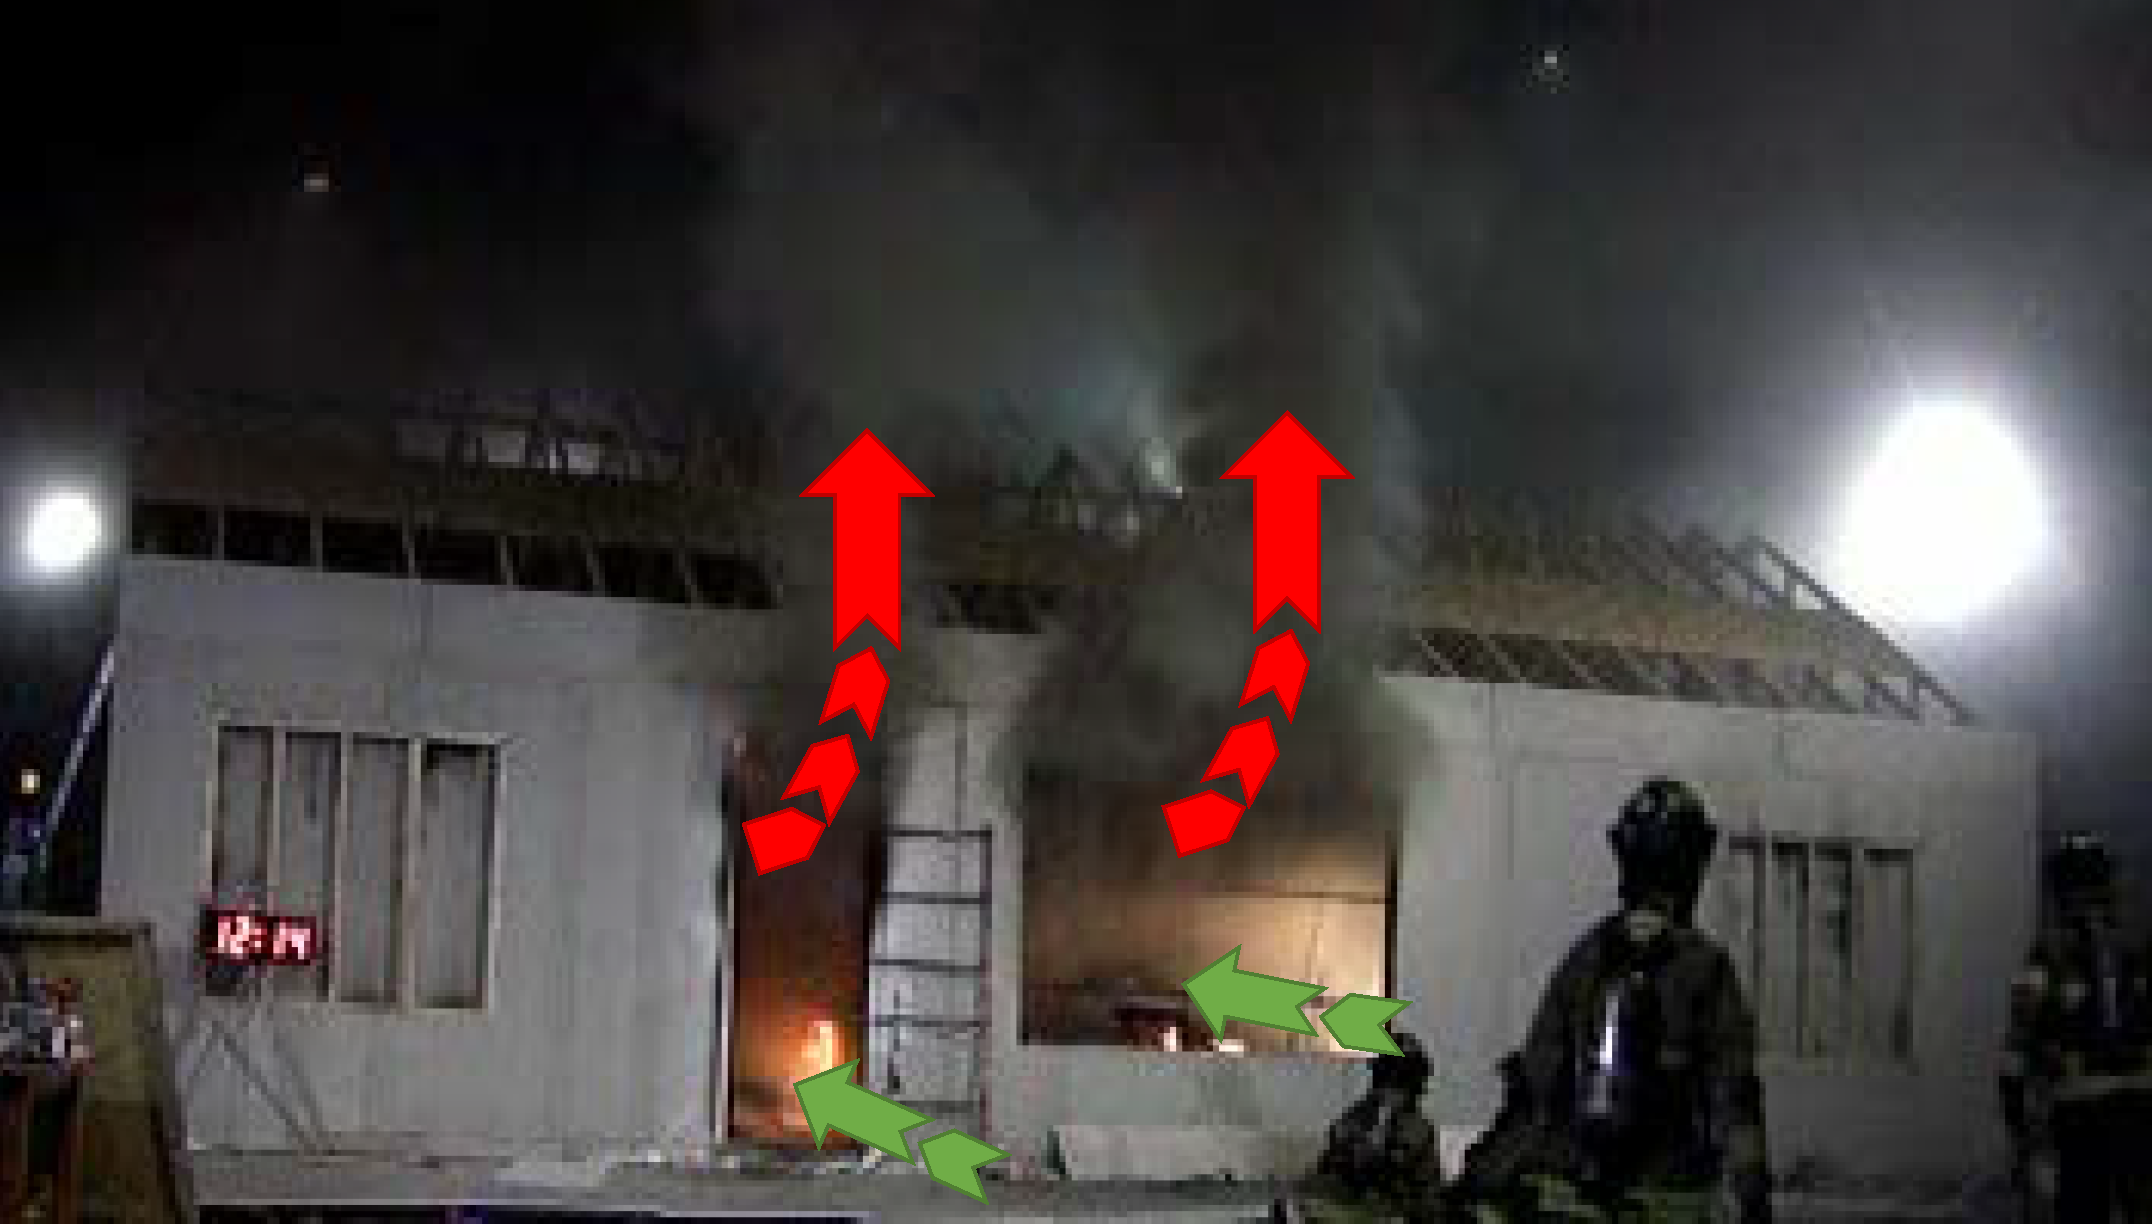
\includegraphics[height  = 1.9in ]{0_Images/Tactical_Considerations/Fan_Earlier/Horizontal_Flows_Arrows.png}} &
		\subfloat[Flow with Vertical Ventilation]{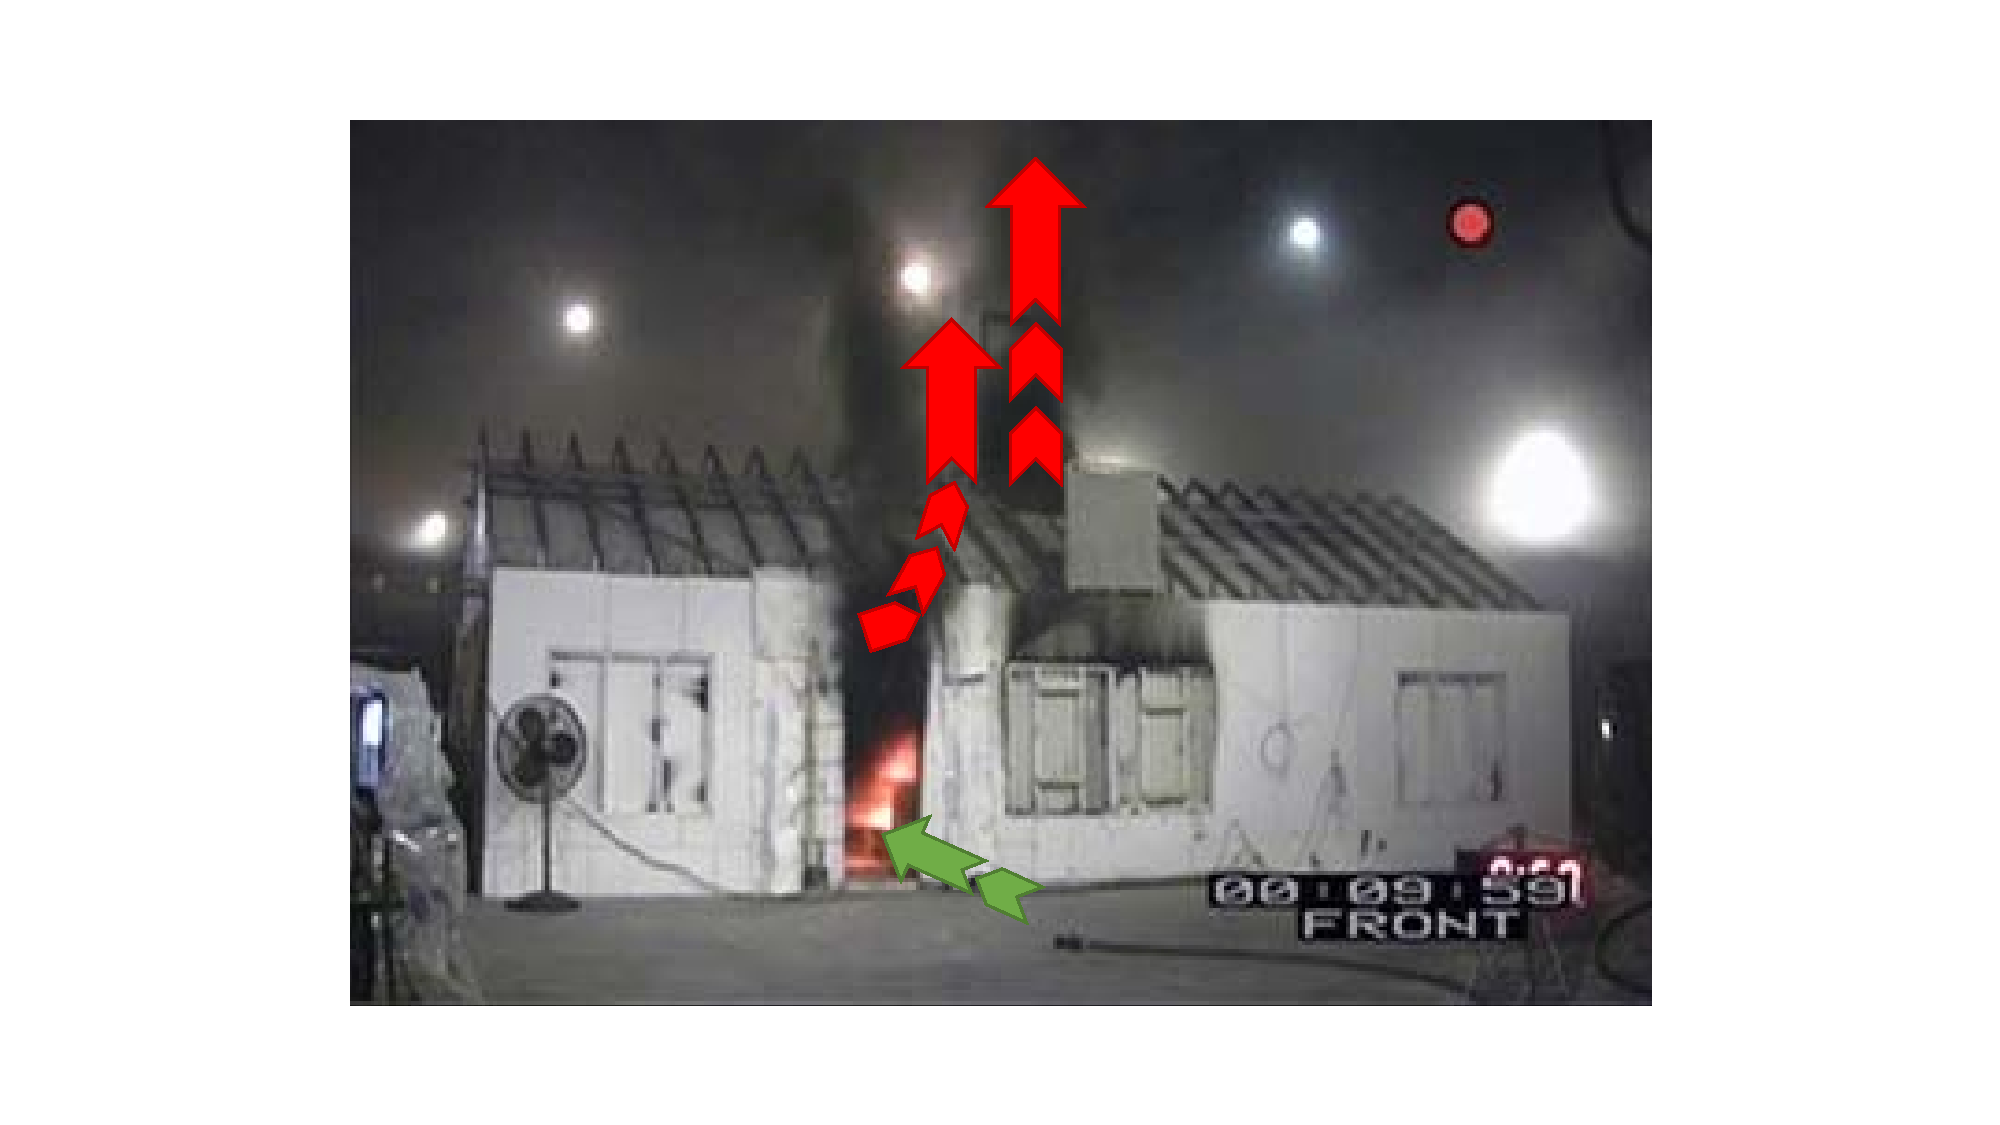
\includegraphics[height = 1.9in ]{0_Images/Tactical_Considerations/Horizontal_Vertical_PPV/Vertical_Flows.pdf}} \\
	\end{tabular}
	\subfloat[Flow with Positive Pressure Ventilation]{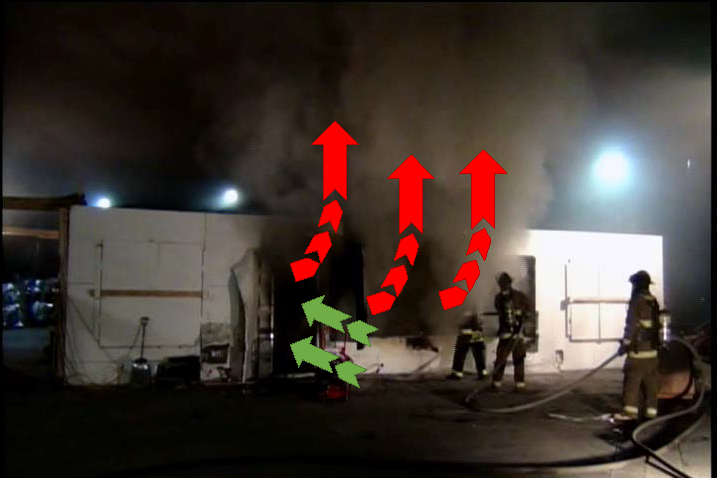
\includegraphics[height = 2.0in ]{0_Images/Tactical_Considerations/Fan_Earlier/PPV_Flows_Arrows.png}}
	\caption{Comparing Horizontal Vertical and Positive Pressure Ventilation Flows in a Living Room Fire}
\end{figure}

\paragraph{Positive Pressure Attack/Ventilation} \mbox{}
Positive pressure ventilation (PPV) is the use of high powered ventilation fans to remove products of combustion from a fire building after the fire has been controlled. Simillary, positive pressure attack is the use of PPV to control the flow of products of combustion, prior to fire control, with the intent of providing increased visibility and tenability for firefighters and potential occupants while fire suppression efforts are underway

The intent of positive pressure attack or PPA is to alter the flow of the products of combustion within a structure. In theory, the fan creates a uni-directional inlet of ambient air which replaces the heat, smoke and toxic gases as they are forced out of the unidirectional exhaust. This is accomplished by increasing the pressure in adjacent compartments to force the products of combustion out of intended exhaust locations. Altering flow has the potential to reduce temperatures and gas concentrations, while simultaneously increasing visibility. The tactic can be employed prior to fire control and is defined as positive pressure attack (PPA) or post fire control defined as positive pressure ventilation (PPV).  Figure \ref{fig:PPAConcept} illustrates a possible ventilation profile for PPA on a bedroom fire in a single story structure. 

\begin{figure}[H]
	\centering
	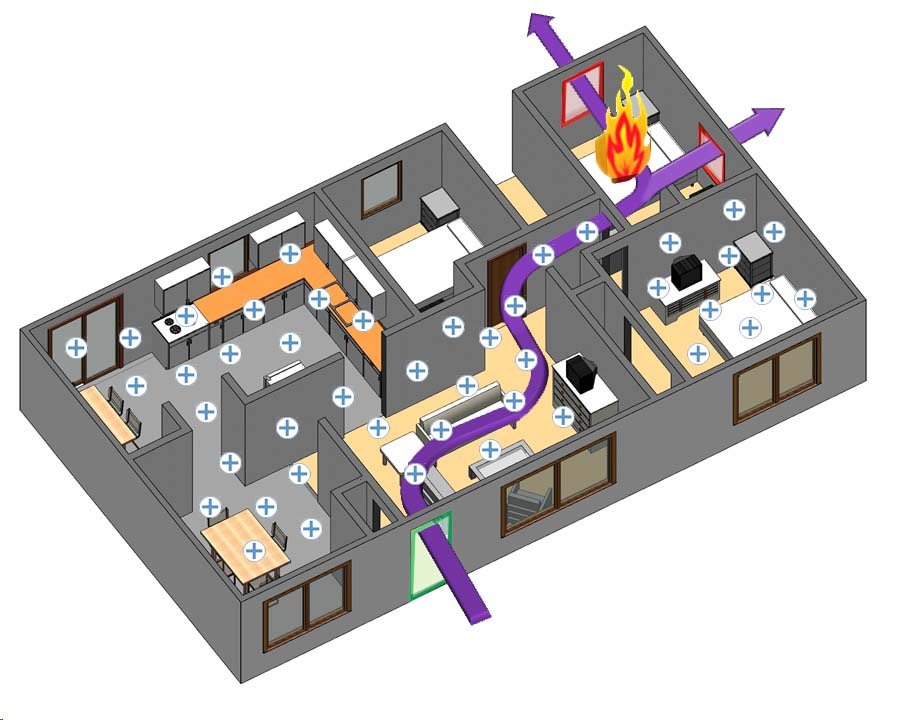
\includegraphics[width = 3in]{0_Images/Tactical_Considerations/Understanding_Basics/Positive_Pressure.jpg}
	\caption{Positive Pressure Attack/Ventilation}
	\label{fig:PPAConcept}
\end{figure}

When PPA is employed correctly, using the fan to direct the heat created by the fire out of an exhaust opening rather than allowing it to flow back into the structure, it is very effective at controlling the temperature. As seen in Figure \ref{fig:PPAControllingFlows} the fan was capable of reducing the temperature in the hallway by directing the majority of the flow out of the bedroom 2 windows rather than back into the hallway. This can be confirmed in Figure \ref{fig:PPAControllingFlows}b where the velocity of the flow coming out of the bedroom is reduced once the fan is applied. 

\begin{figure}[H]
	\centering
	\begin{tabular}{c c}
		\subfloat[Hallway Temperature]{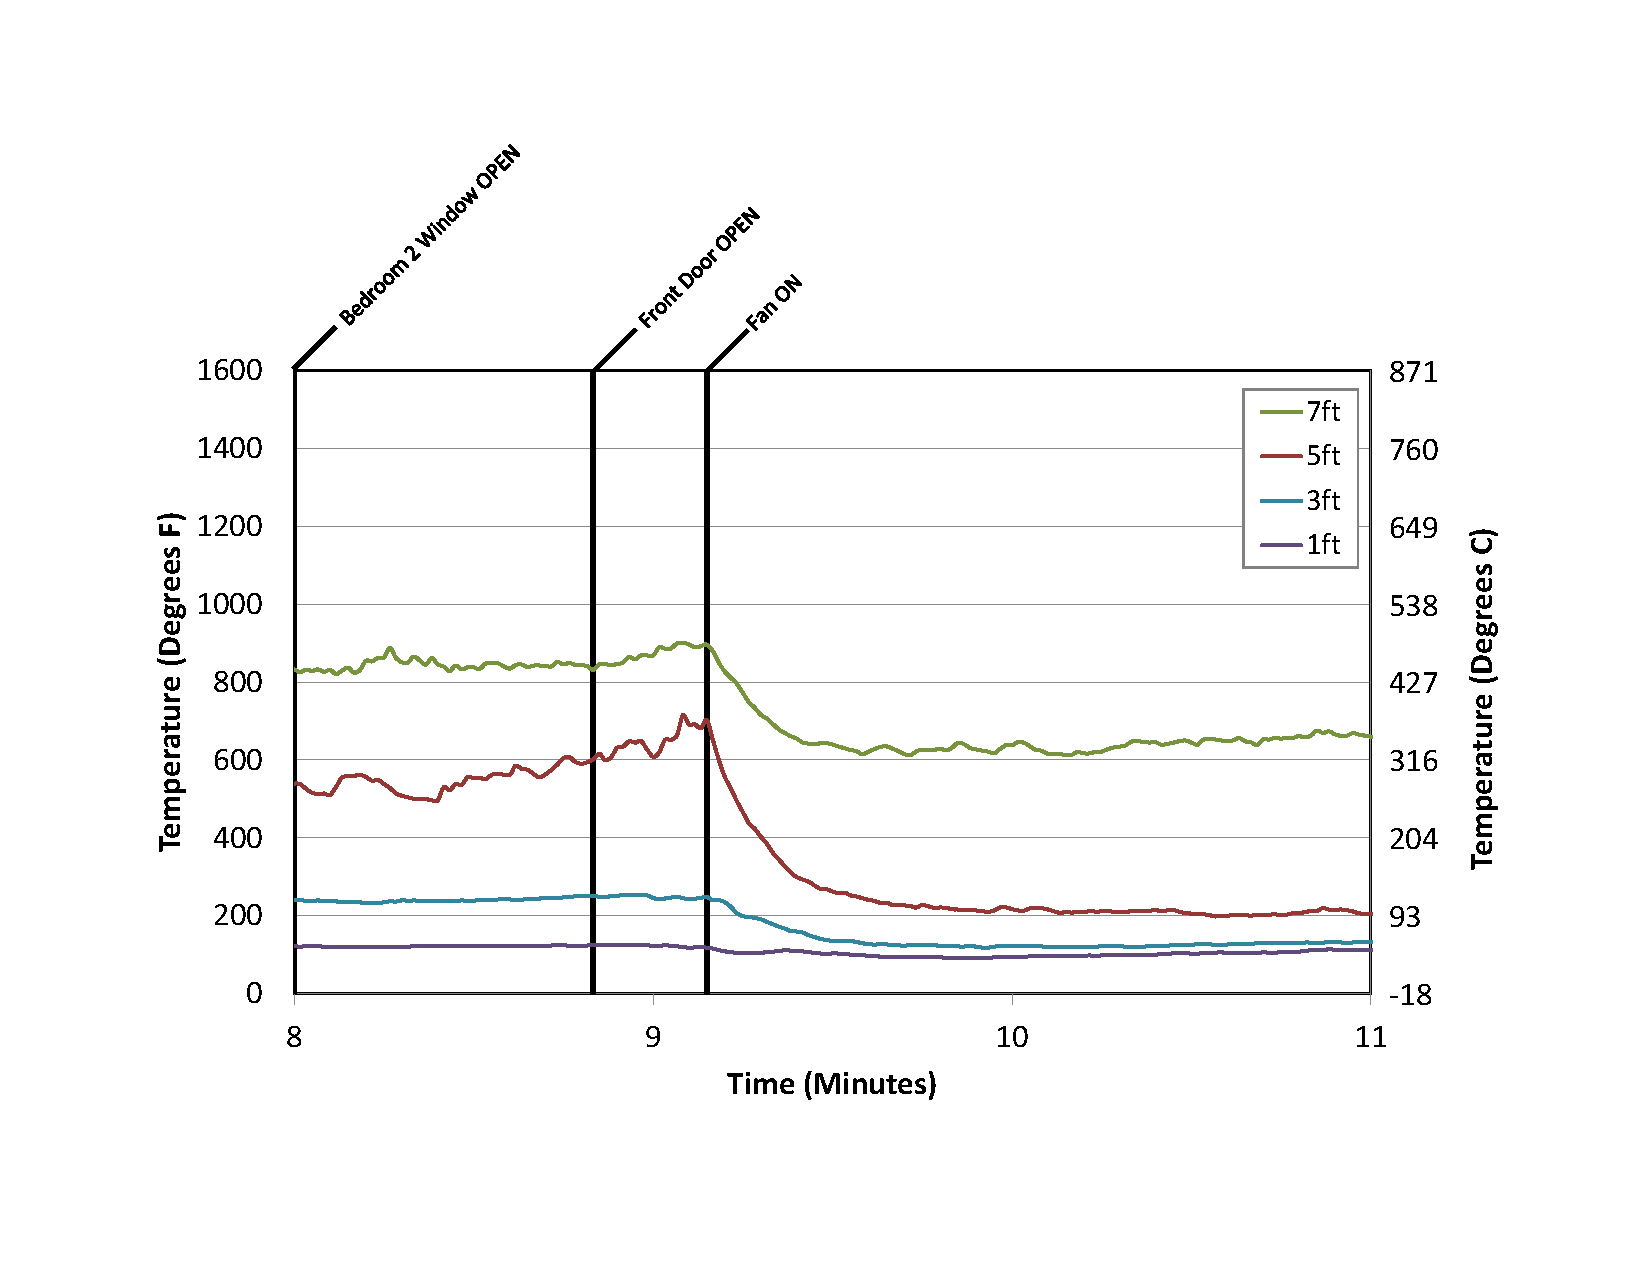
\includegraphics[width = 3in ]{0_Images/Tactical_Considerations/Horizontal_Vertical_PPV/HallTemps.pdf}} &
		\subfloat[Bedroom 2 Doorway Velocity]{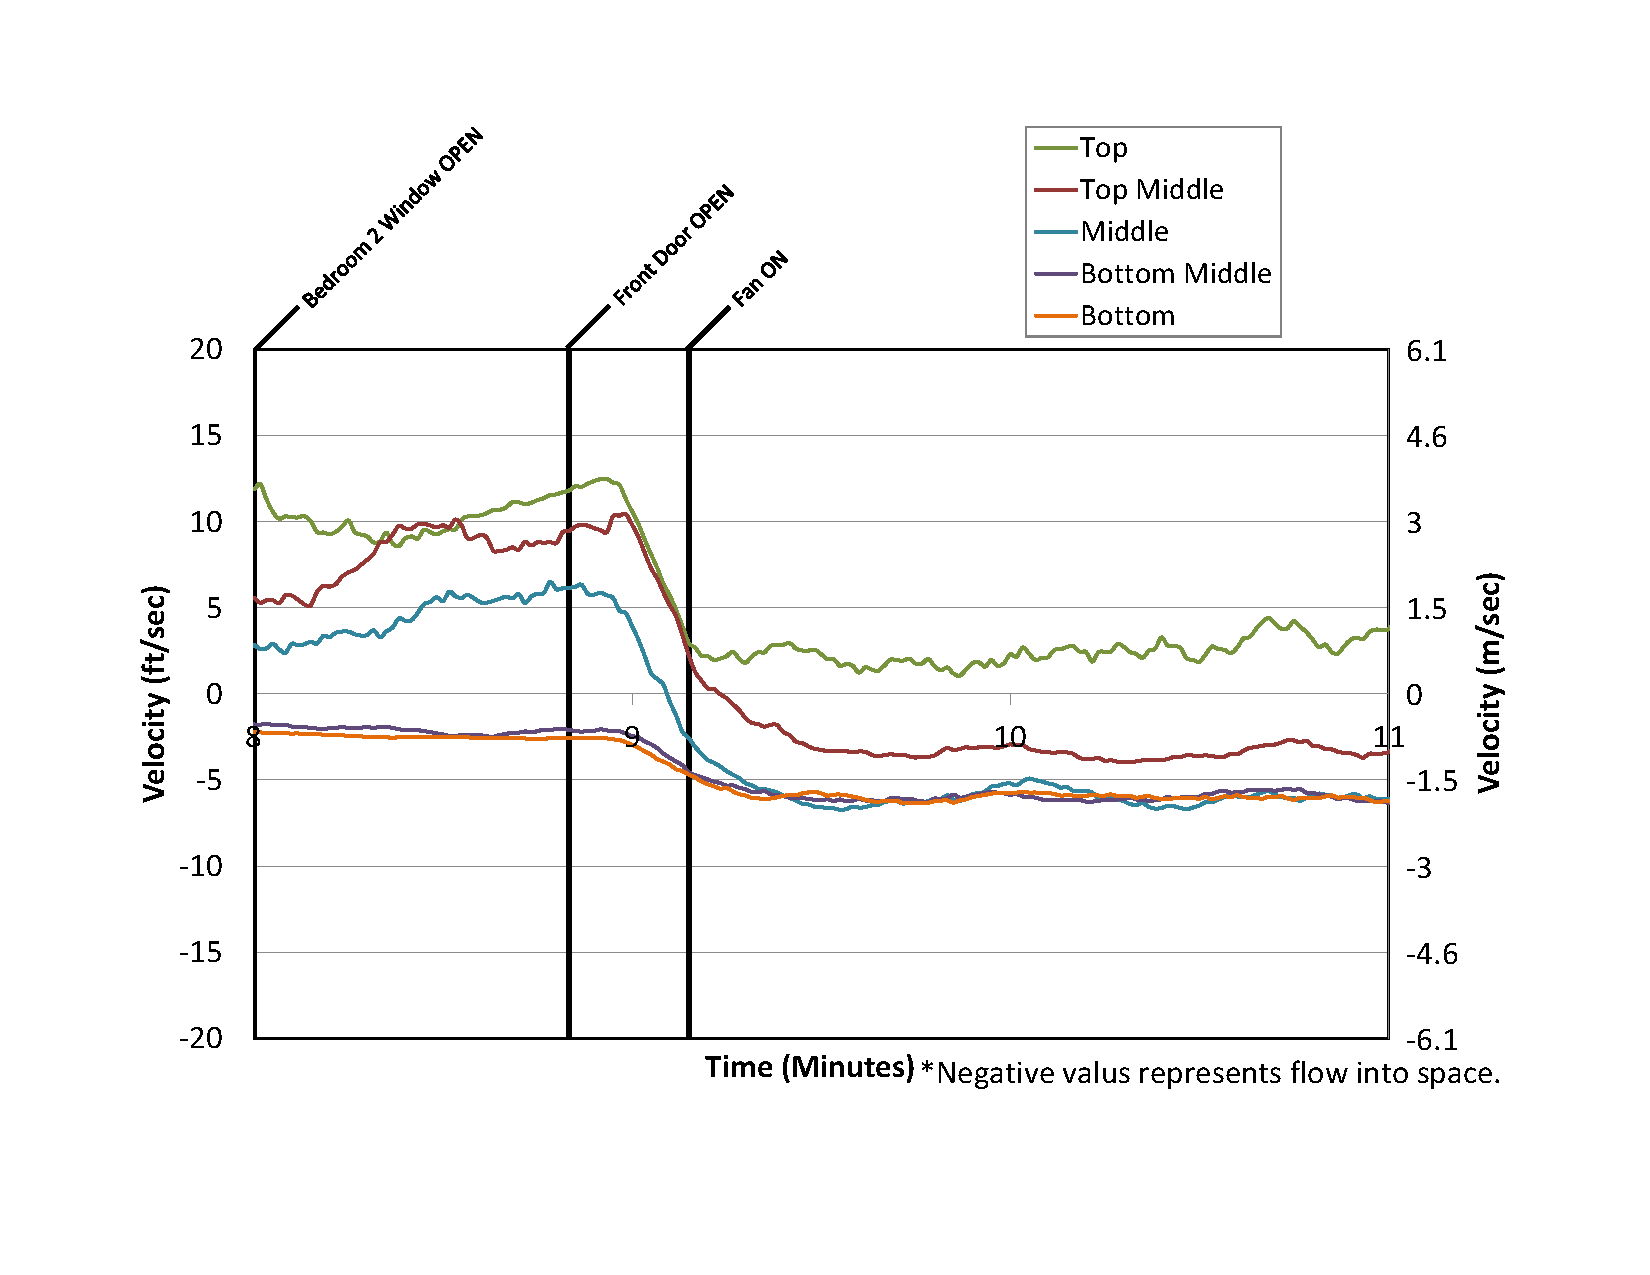
\includegraphics[width = 3in ]{0_Images/Tactical_Considerations/Horizontal_Vertical_PPV/BedDoorFlow.pdf}} \\
	\end{tabular}
	\subfloat[Ventilation Profile]{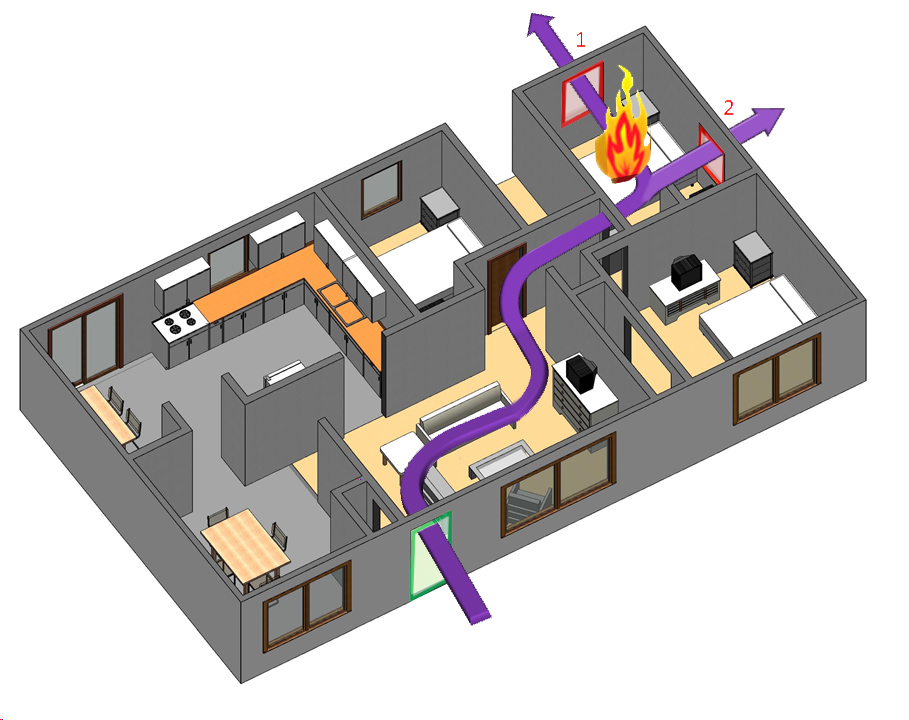
\includegraphics[width = 2.5in]{0_Images/Tactical_Considerations/Understanding_Basics/Experiment_6.jpg}}
	\caption{Positive Pressure Attack - Controlling Flows}
	\label{fig:PPAControllingFlows}
\end{figure}

It is not as effective at increasing visibility because the interior environment is often already charged with smoke, which, although diluted by the fan with clean cool air, does not reduce the optical density enough to increase visibility. The area of the structure charged with smoke, must be all exhausted through the fire room, which takes time. Figure \ref{fig:SmokeToExhaust} graphically shows the volume which would need to be exhausted through the fire room in a single story ranch home. Although the fan is capable of exhausting the built up smoke, in the research conducted, this occurred on the order of 3-5 minutes. It is neither recommended nor practical to wait 3-5 minutes prior to applying water to the fire. 

\begin{figure}[H]
	\centering
	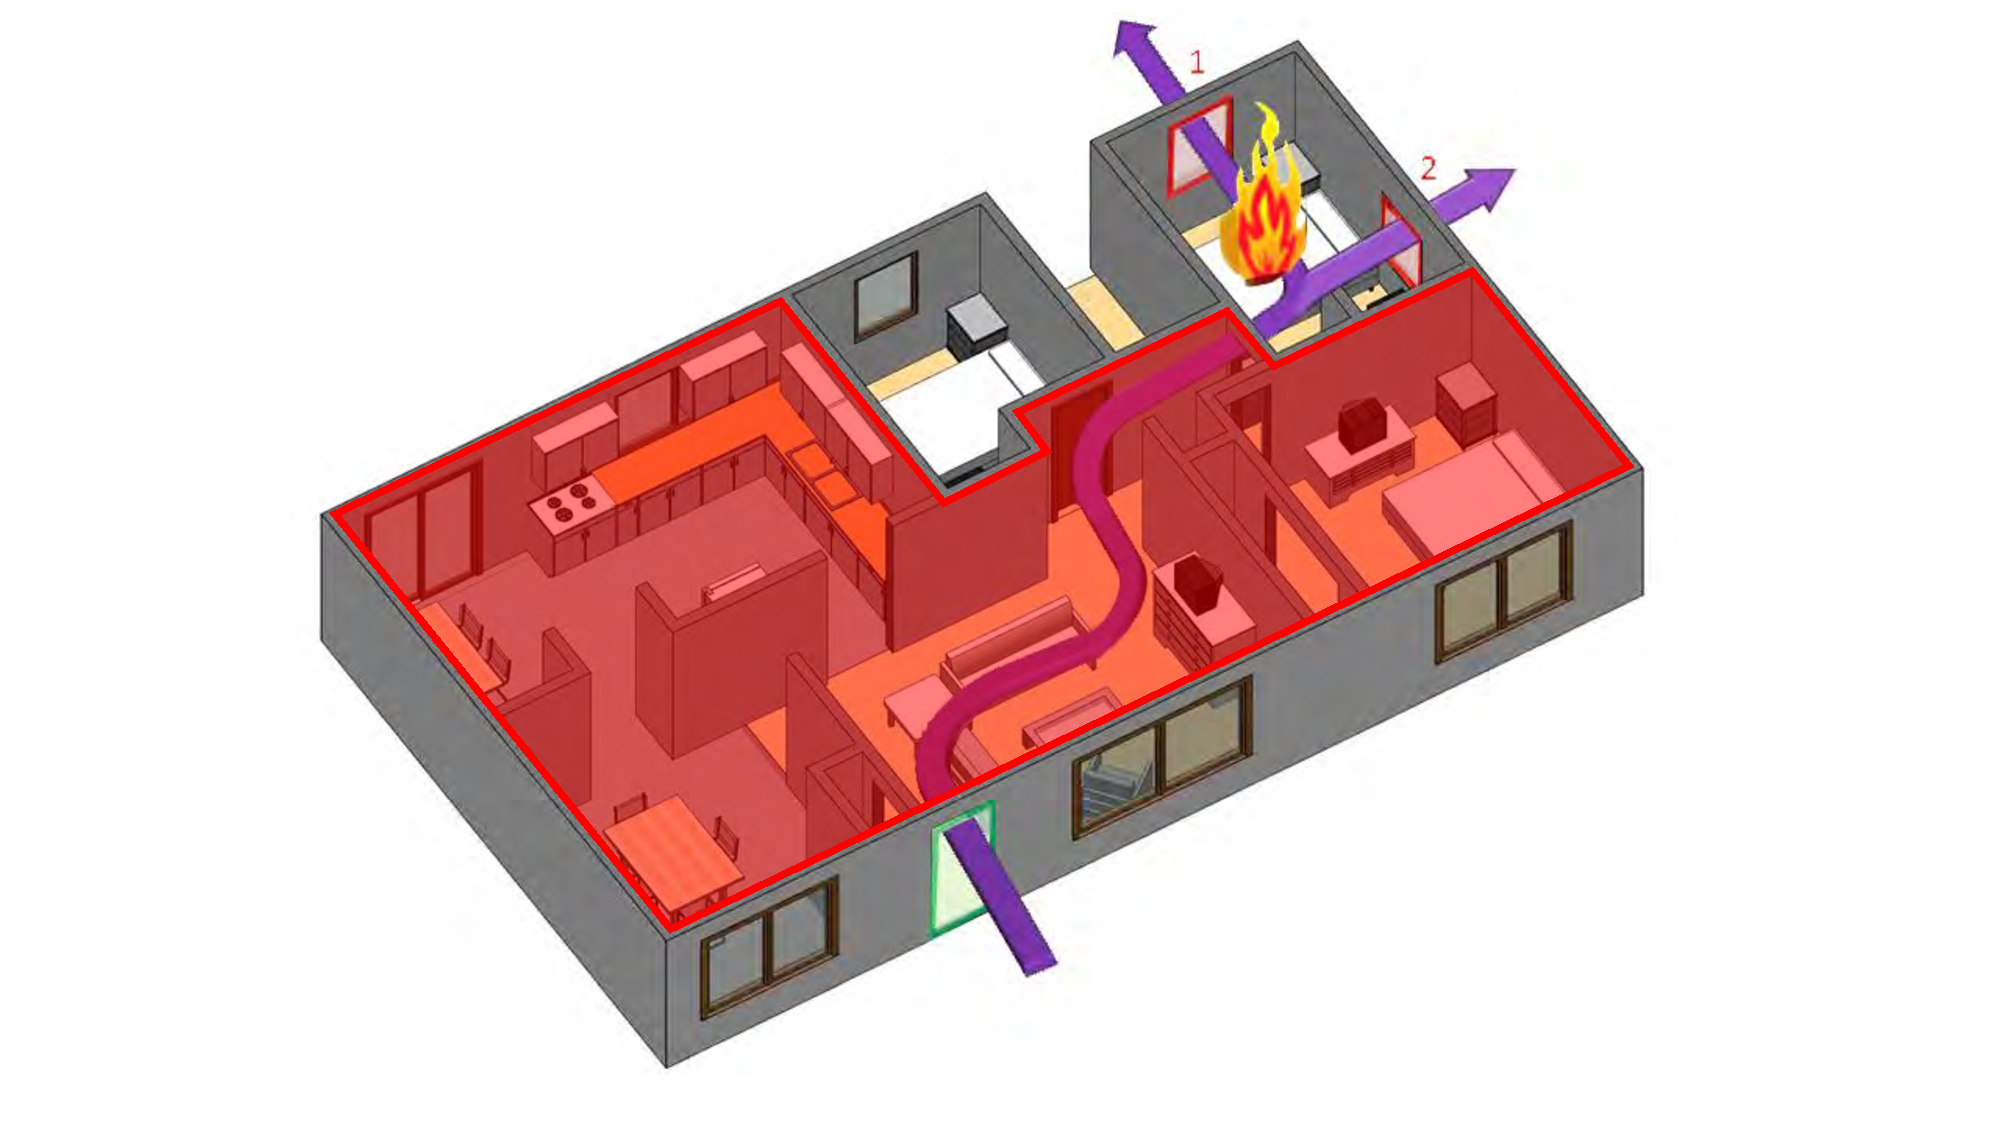
\includegraphics[width = 4in ]{0_Images/Tactical_Considerations/Understanding_Basics/SmokeToBeExhausted.pdf}
	\caption{Volume of Built-Up Smoke to Exhaust}
	\label{fig:SmokeToExhaust}
\end{figure}

\subsection{Horizontal, Vertical and Positive Pressure Attack are different tactics.} 
No one tactic will work in every scenario. Understanding the fire environment with emphasis on ventilation limited fire dynamics and how fire department operations impact those will ensure the tactic chosen is most effective.

In a scenario with a bedroom fire isolated from the remainder of the structure with a single doorway and multiple windows or one large window, positive pressure attack may be the most effective means of controlling the flows within the structure. If the bedroom does not have a large window, utilizing horizontal or vertical ventilation with door control may be the more effective option. 

With proper training and education, they can all be implemented successfully to improve life safety, property conservation, and incident stabilization.  Water must be applied in coordination with each of these ventilation tactics for successful outcomes.   For example, in a compartmentalized structure, PPA will transition a ventilation limited compartment fire to flashover faster, however, temperatures will be lower in adjacent spaces and return to ambient in those spaces faster with water application.

\subsection{The setback of the fan or development of a “cone of air” is not as important as the exhaust size.}
In the application of PPA a great deal of emphasis has been placed on the flow occurring at the front door. It was thought, if a ``cone of air'' was placed over the door the result would be inflow through the door, pressurizing the structure and forcing all flow out of the exhaust openings. Manuals make reference to ensuring PPA effectiveness by evaluating for total inflow at the inlet (Figure \ref{fig:ConeImages}).

\begin{figure}[H]
	\centering
	\begin{tabular}{c c}
		\subfloat[Fan Setup \cite{PPA_Garcia}]{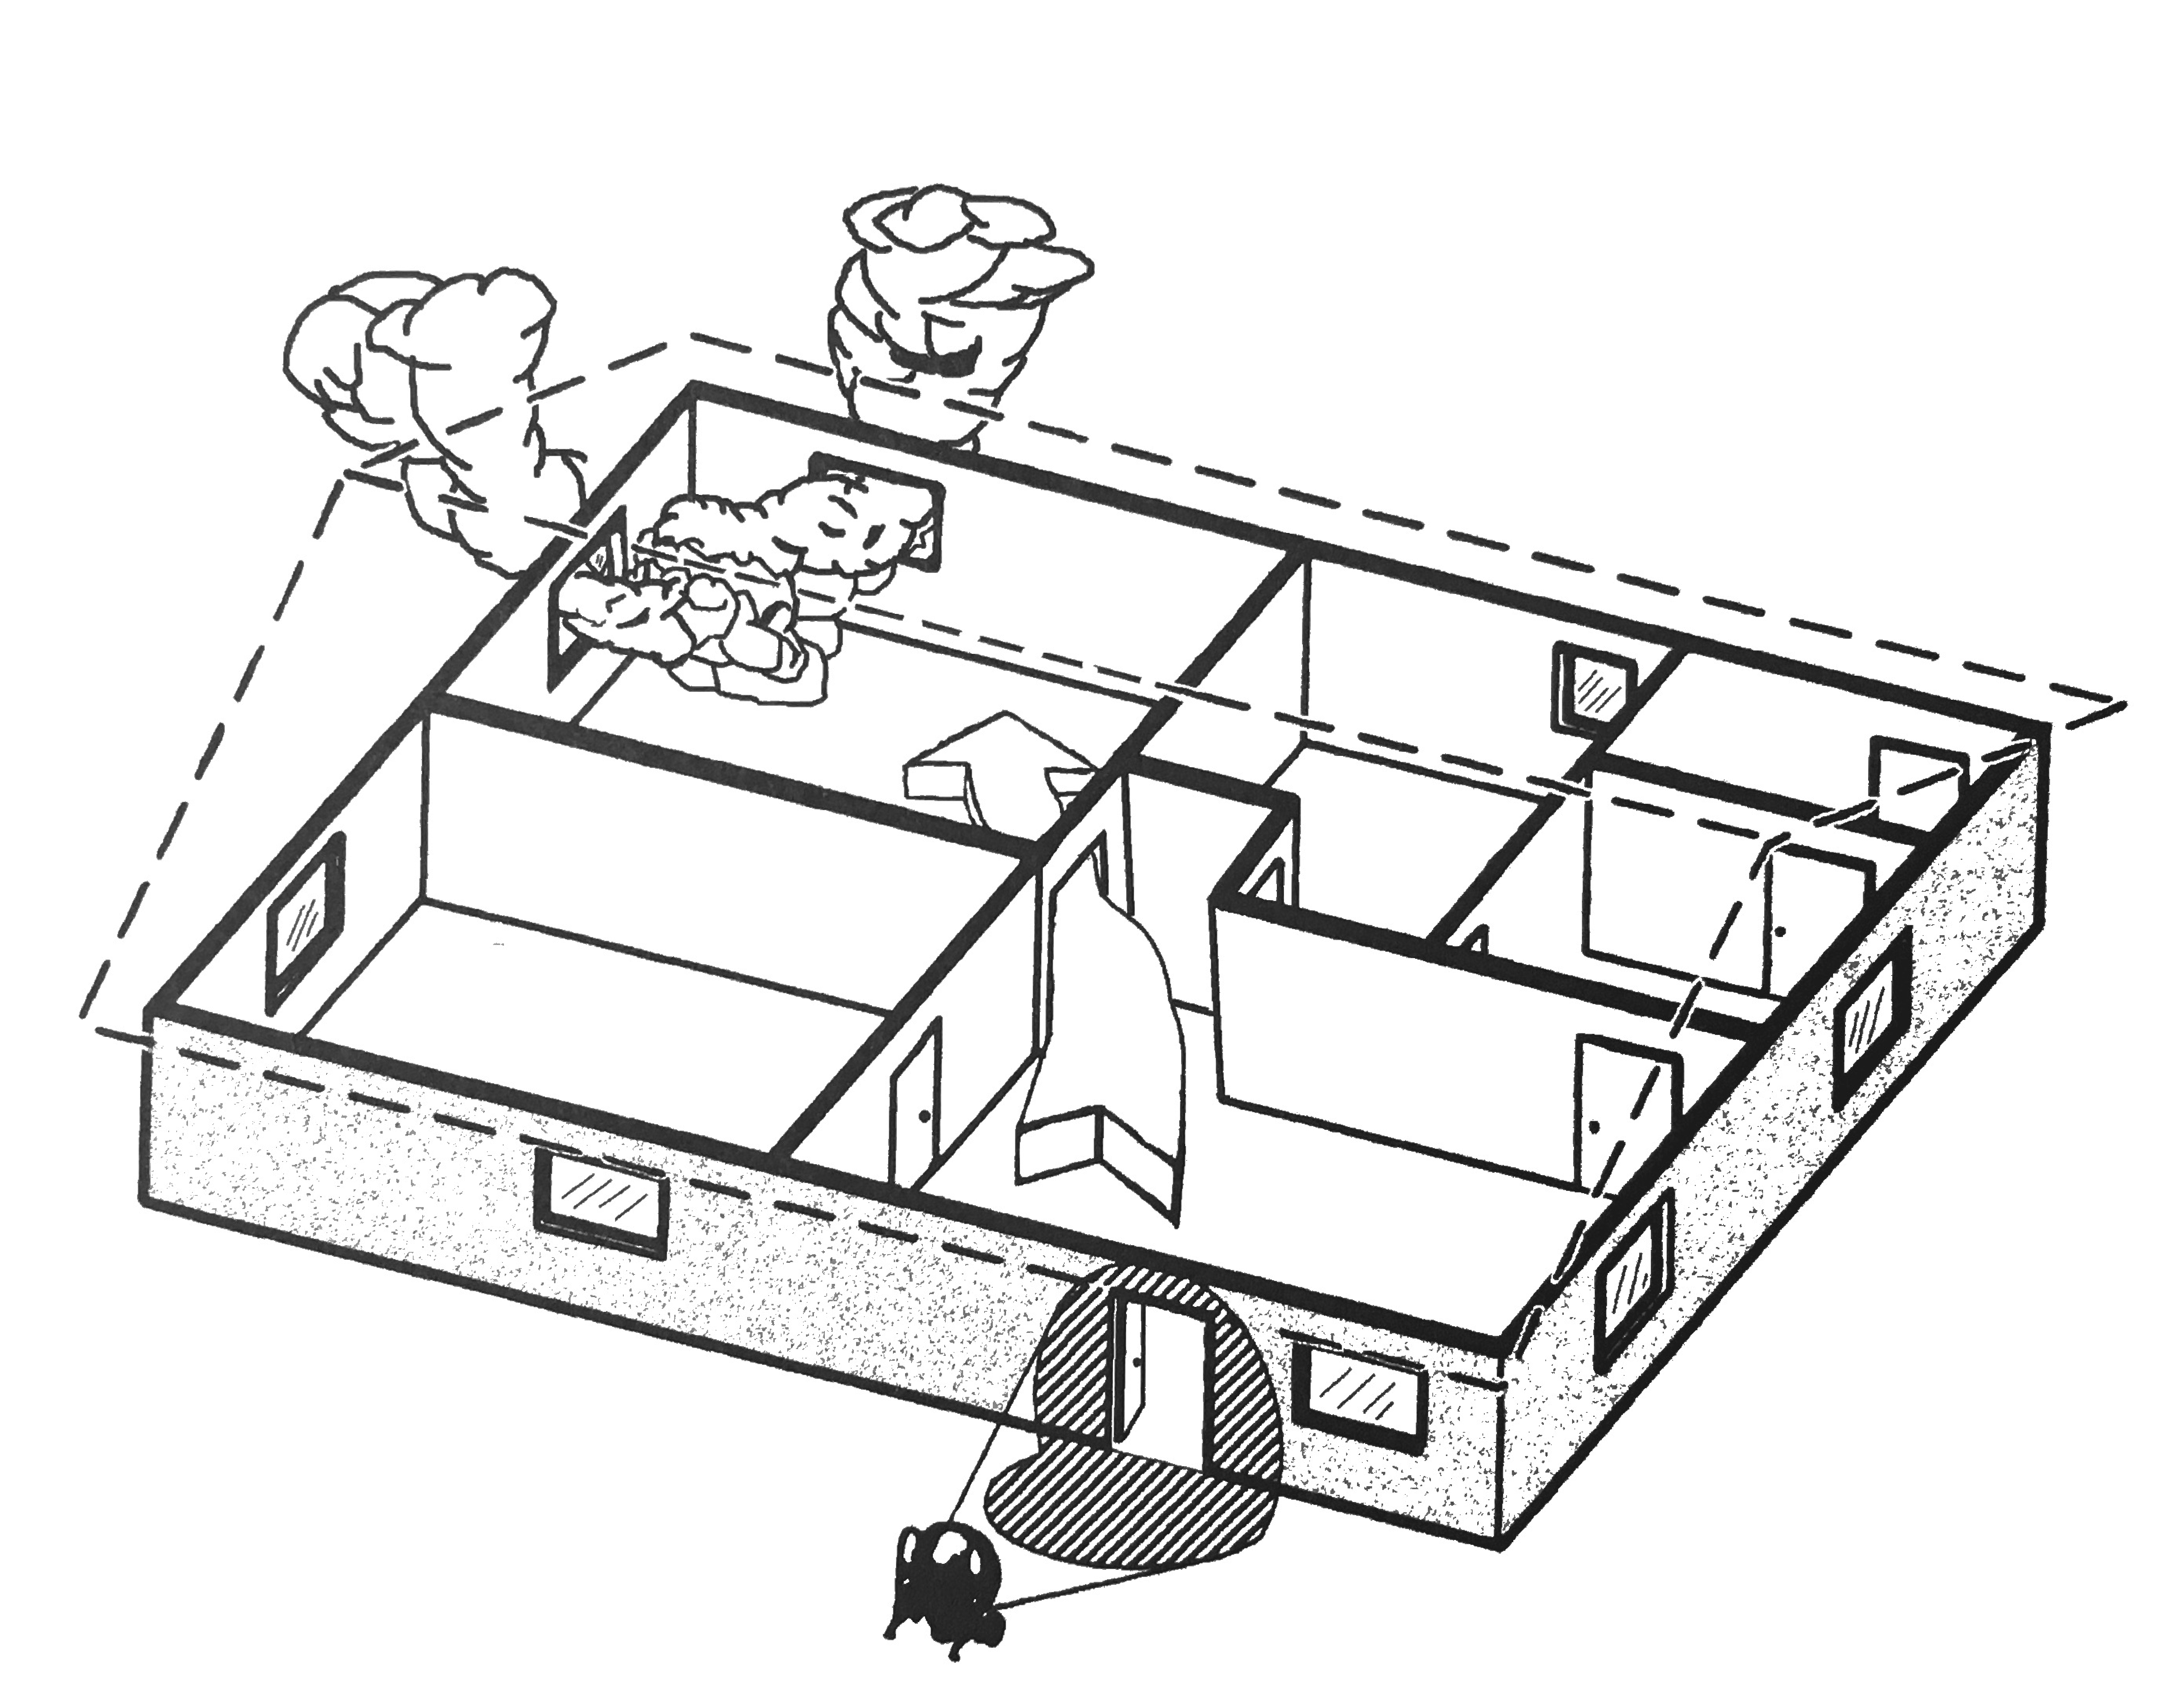
\includegraphics[width = 2.5in]{0_Images/Tactical_Considerations/Exhaust_Over_Cone/Cone3.pdf}} & 
		\subfloat[PPA \cite{TempestWebsite}]{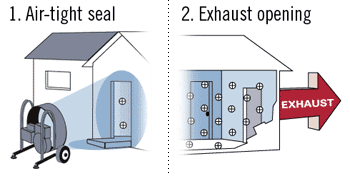
\includegraphics[width = 3.0in]{0_Images/Tactical_Considerations/Exhaust_Over_Cone/howdoes.png}} \\	
	\end{tabular}	
	\subfloat[Setback Distance \cite{SuperVacManual}]{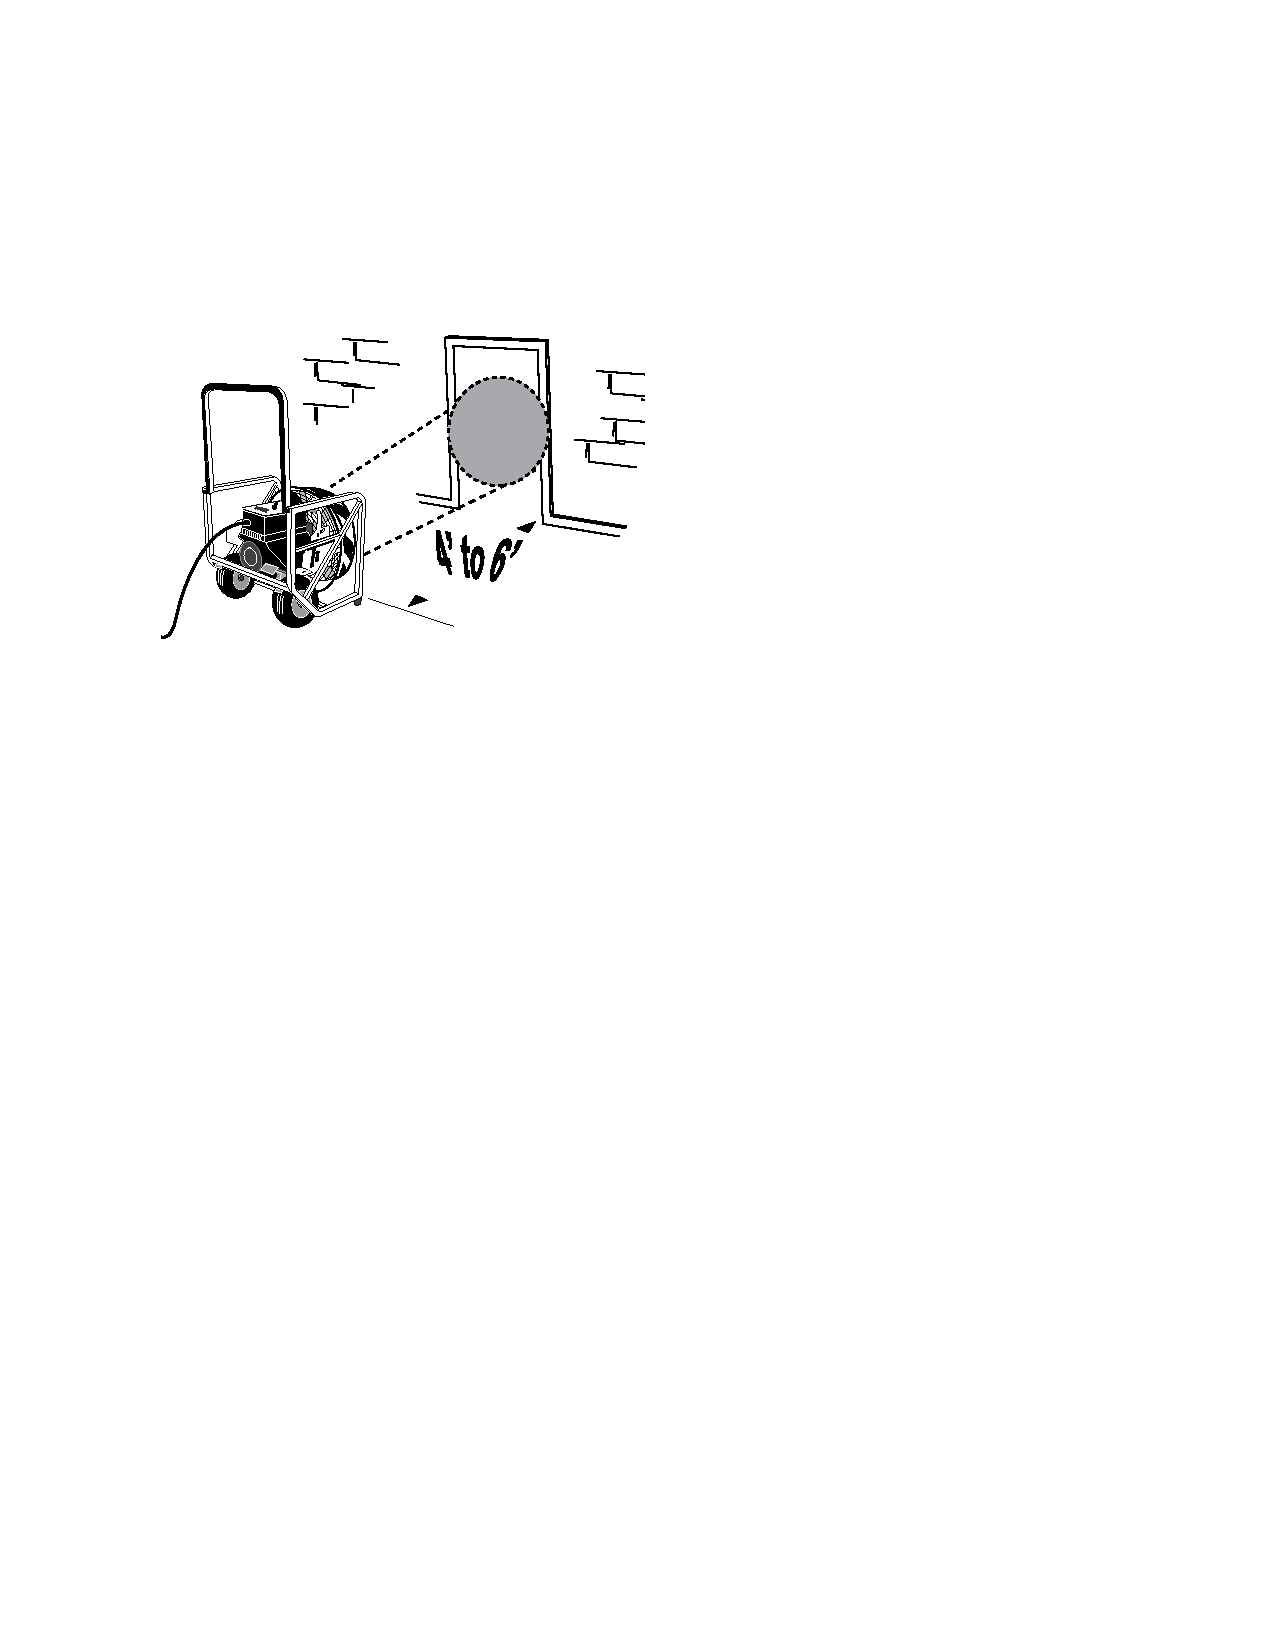
\includegraphics[width = 2.5in]{0_Images/Tactical_Considerations/Exhaust_Over_Cone/SV-Training-Manual.pdf}} 
	\caption{Images of ``Cone of Air'' in Fire Service Literature}
	\label{fig:ConeImages}
\end{figure}

Section \ref{sec:OngoingAssessment} will discuss how the inlet being complete inflow was not noted in any of the fire experiments. The pressure gradient seen when the flows from the fire are opposed by the flow from the fan, as illustrated in Figure \ref{fig:FanAndDoorFlow}, prevent complete inflow. To effectively counteract the flow from the fire, an airtight seal as indicated in Figure \ref{fig:ConeImages}b would be required. This is not possible with a positive pressure fan. Instead of focusing on the flow at the inlet, focus should be on the pressure created and the exhaust size. 

The effectiveness of PPA can be tied directly to the pressure created inside the structure. Flow will always be from a higher pressure to lower pressure. The difference in pressure between compartments determines the direction of flow. The intent of PPA is to increase the pressure in adjacent compartments higher than the fire compartment to prevent the flow of products of combustion from the fire compartment to the remainder of the structure. During the cold flow experiments, the greatest pressure increase in the adjacent compartments occurred when the fan was placed between 5$ft$ and 9$ft$ from the intake with the tilt position for the fan used in the full scale fire experiments. Figure \ref{fig:SetbackResults} shows the results graphically. 

\begin{figure}[H]
	\centering
	\begin{tabular}{c c}
		\subfloat[Flow Exiting Bedroom 2 Window]{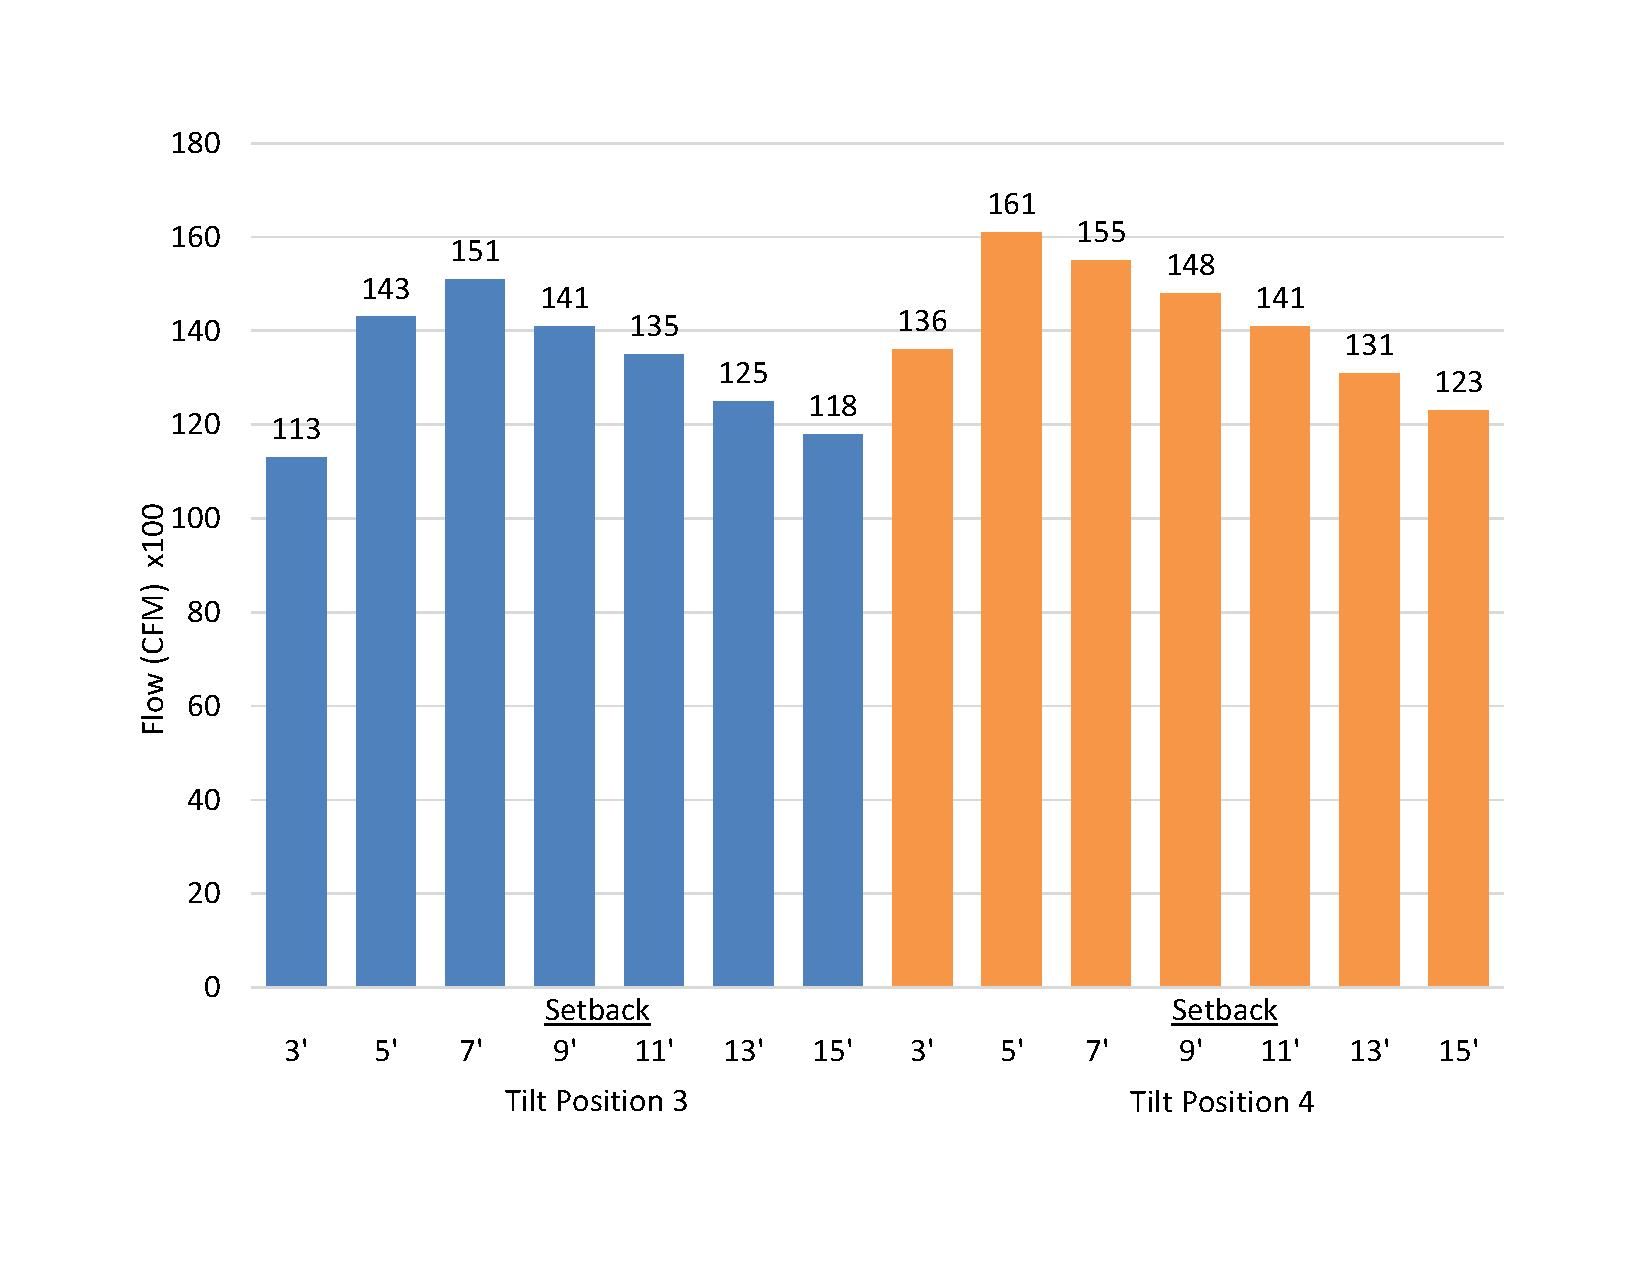
\includegraphics[width = 3 in]{0_Images/Coldflow/Setback/SingleStoryFlow.pdf}} & 
		\subfloat[Master Bedrooom Pressure]{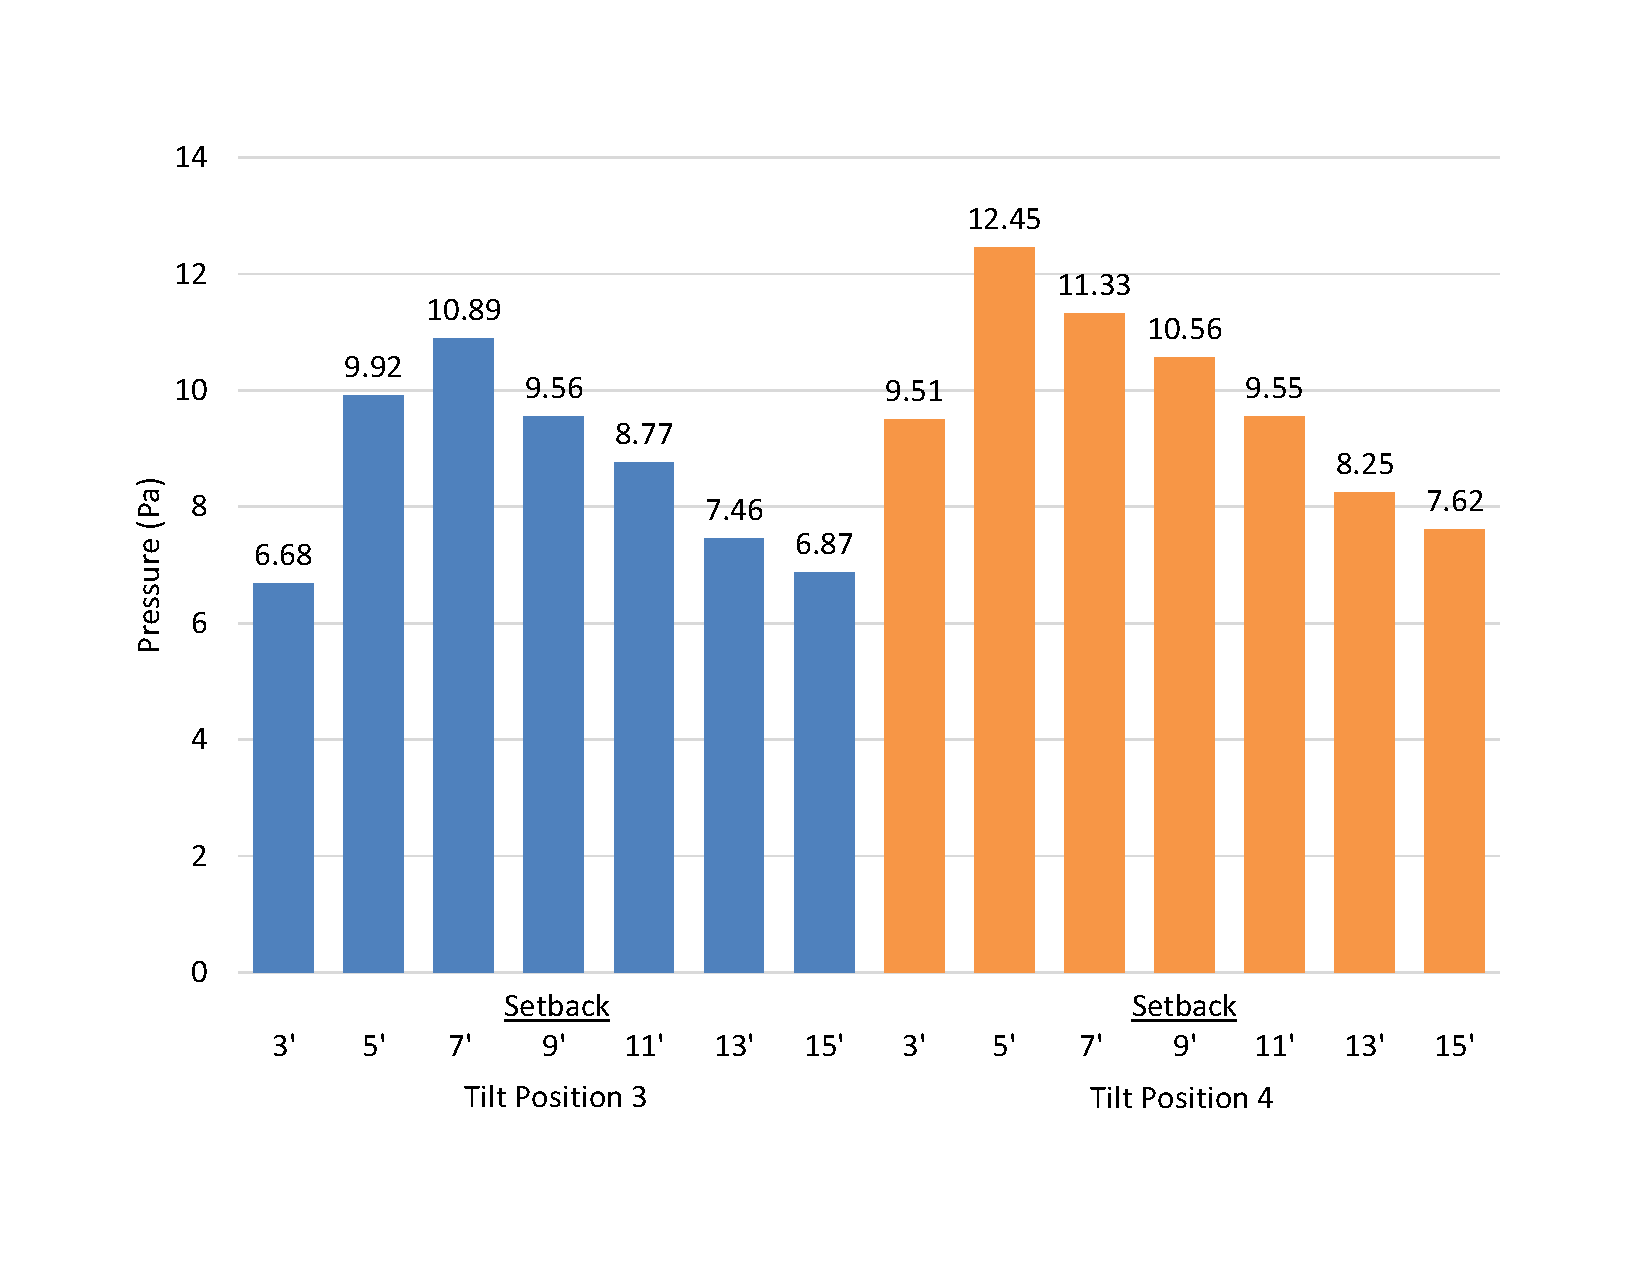
\includegraphics[width = 3 in]{0_Images/Coldflow/Setback/SingleStoryPressure.pdf}} \\
		\subfloat[Flow Exiting Bedroom 3 Window]{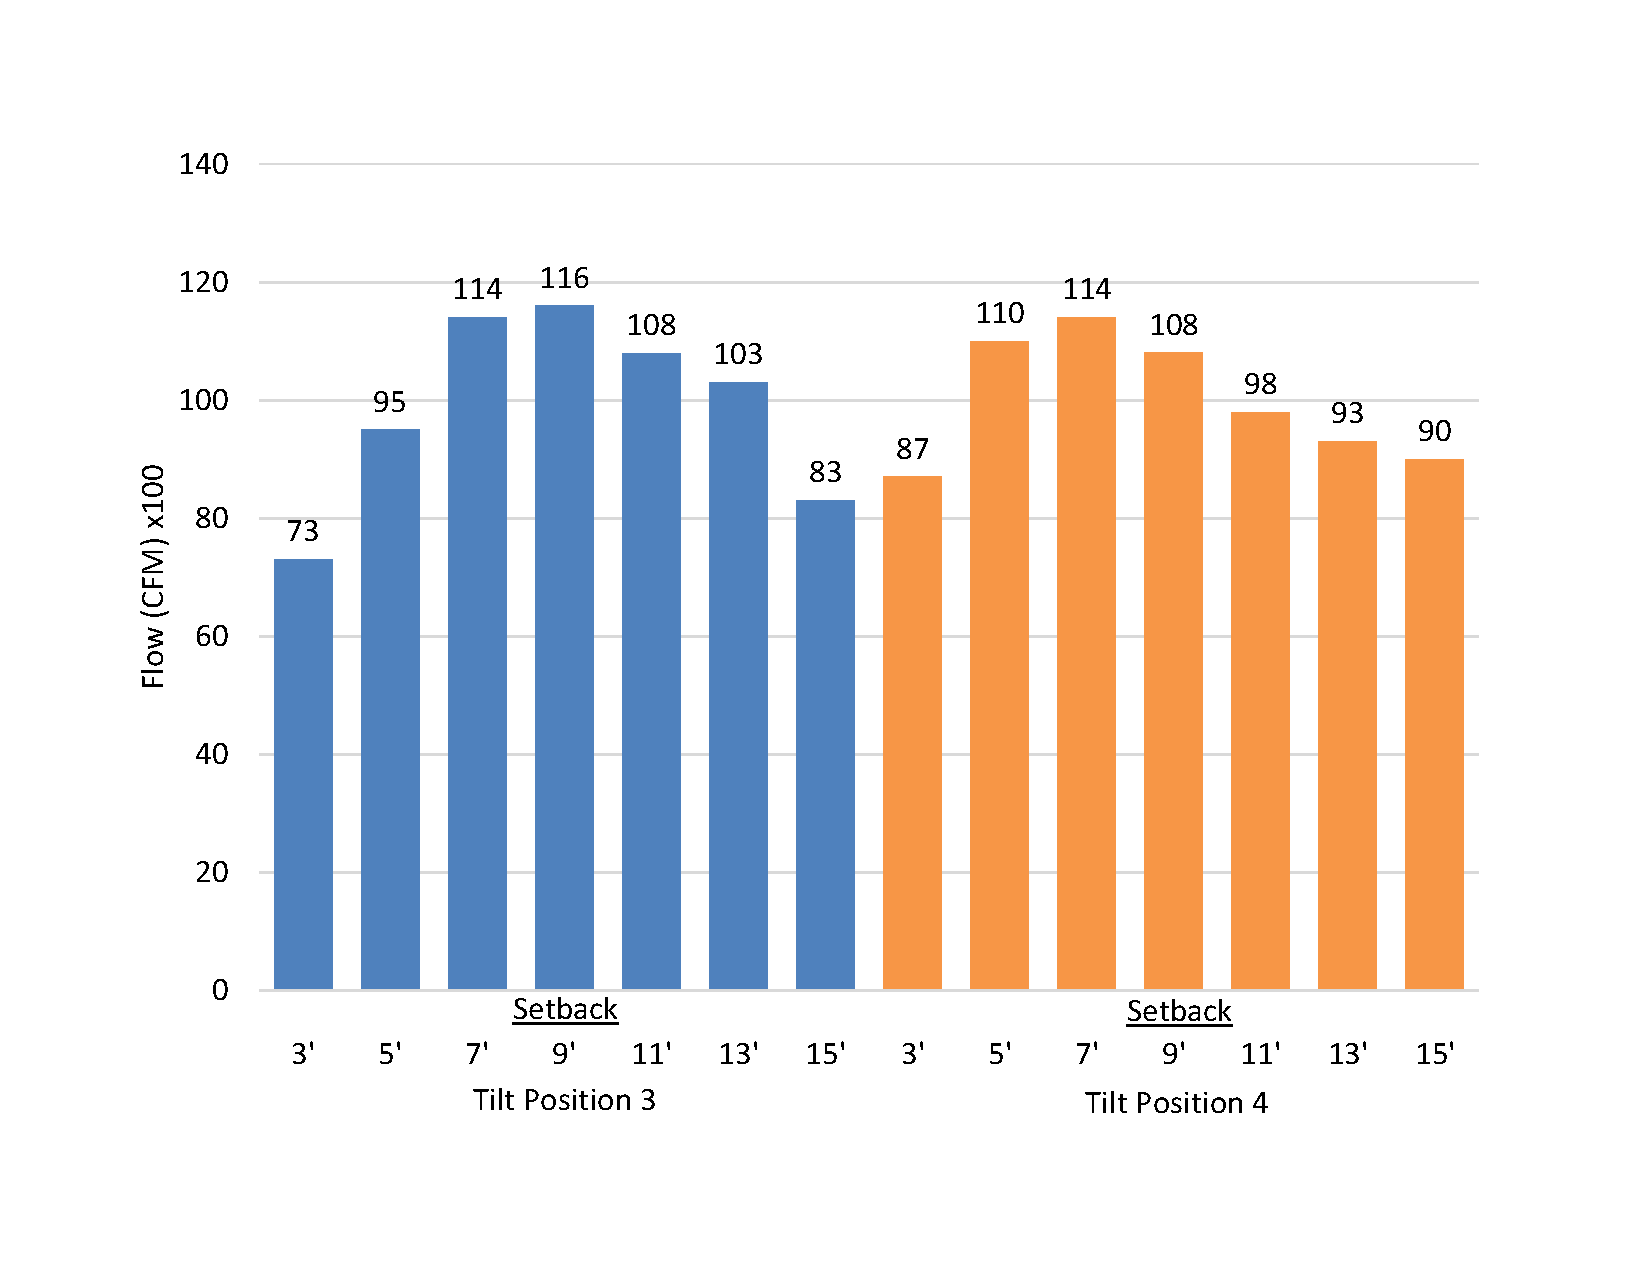
\includegraphics[width = 3 in]{0_Images/Coldflow/Setback/TwoStoryFlow.pdf}} & 
		\subfloat[Family Room Pressure]{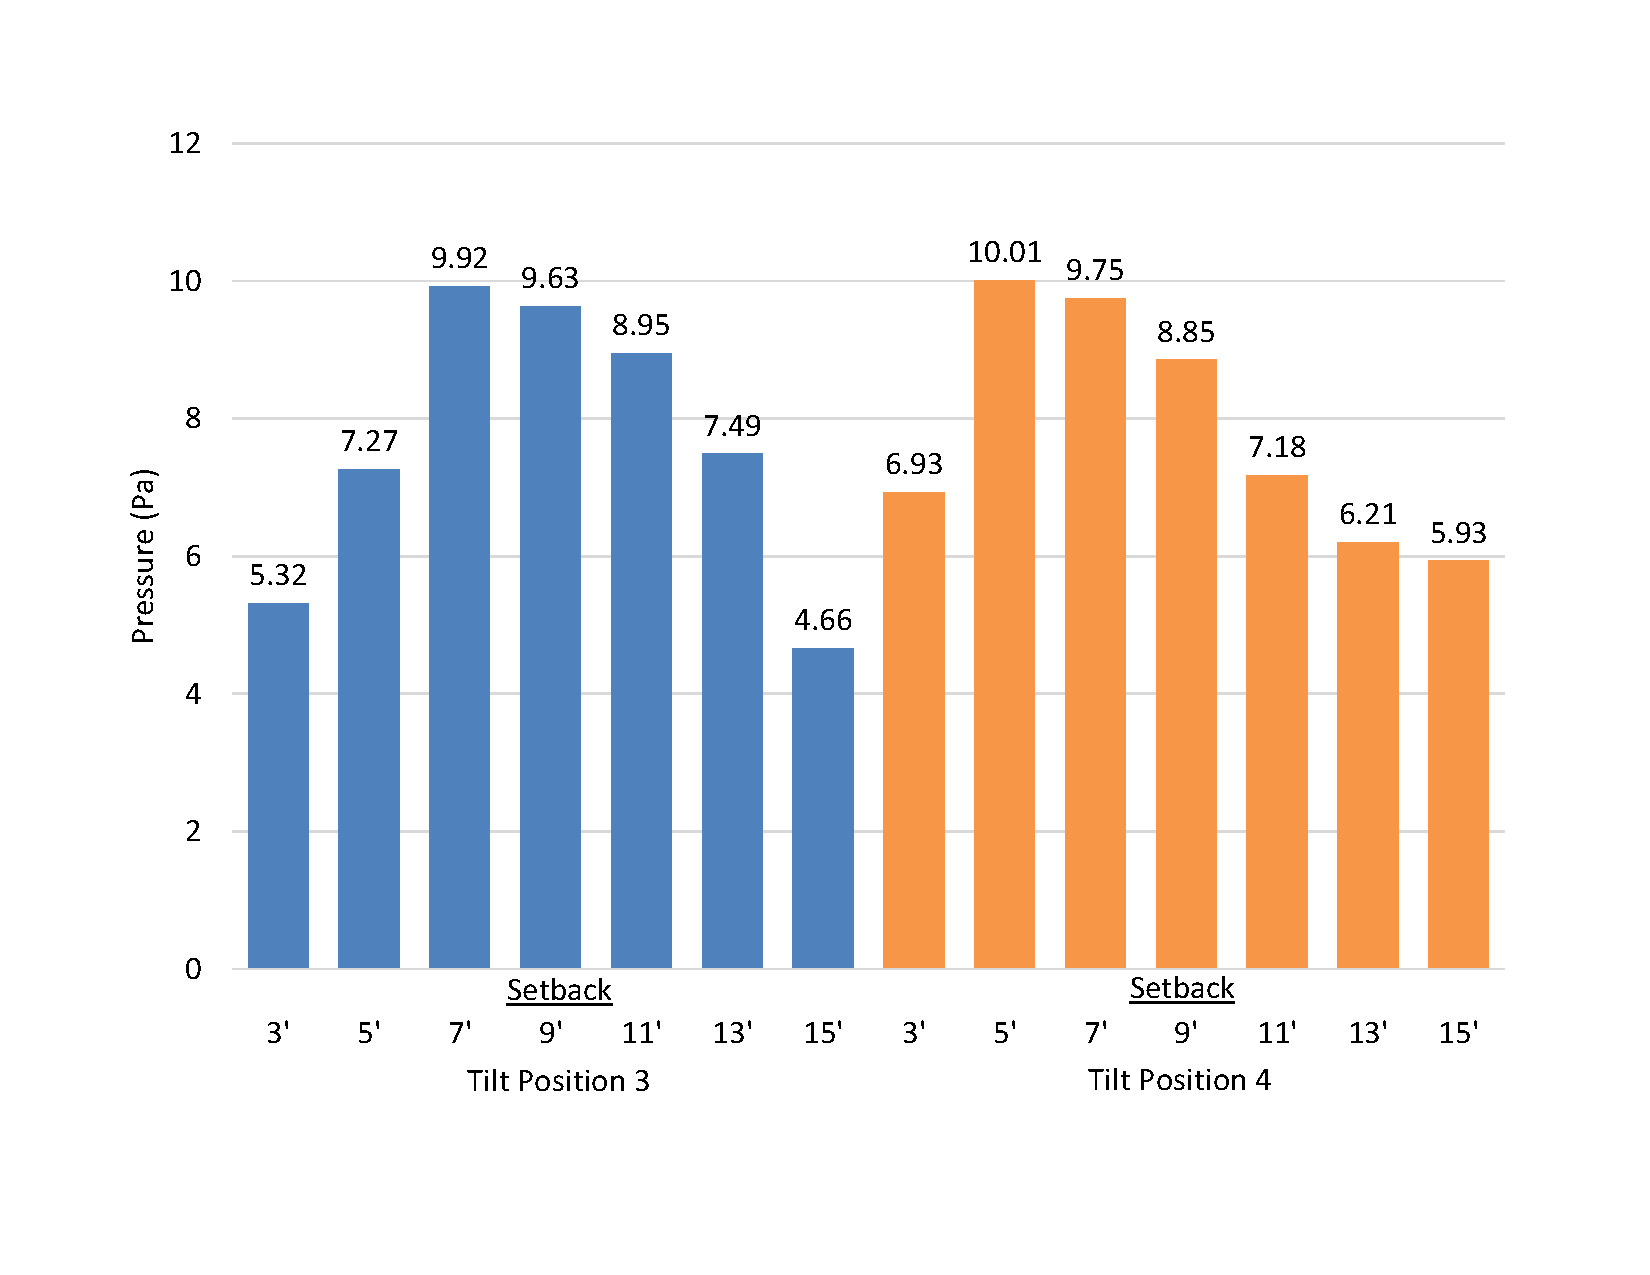
\includegraphics[width = 3 in]{0_Images/Coldflow/Setback/TwoStoryPressure.pdf}} \\  		
	\end{tabular}
	\caption{Fan Setback Results}
	\label{fig:SetbackResults}
\end{figure}

The configuration was independent of structure size, however, only represents the optimal setback for the fan tested. Departments utilizing PPA should verify the most effective placement for their particular fan to produce the greatest pressure increase in adjacent compartments. This cannot be evaluated solely by developing a ``cone of air''. Much like a pump operator must have an understanding of the pressure required to flow a given nozzle, firefighters need to have an understanding of how much pressure their fan can produce prior to the incident. If the fan is not capable of providing the pressure required to overcome the pressure created by a fire, that fan will not be effective for positive pressure attack. 

Relatively inexpensive differential pressure sensors can be used to measure the pressure created by the fan. Setting up the fan in cold flow configurations, with a differential pressure sensor reading the interior and exterior pressure, will help identify the capabilities of a particular fan. The fan should be capable of increasing the pressure in the entrance space to a pressure higher than a fire in a compartment could create. 

In addition to creating as much pressure as possible in adjacent compartments, it is imperative the pressure created by the fan not provide additional pressure to the fire room. This is accomplished by providing an exhaust to inlet ratio of greater than 1:1, and understanding how the interior doorway acts a separation to help maintain the pressure in the adjacent spaces. See tactical consideration \ref{sec:ExhaustDepend}  and \ref{OpenSpaces} for more information.

\subsection{During PPA, an ongoing assessment of inlet and exhaust flow is imperative to understanding whether or not a fan flow path has been established and if conditions are improving} \label{sec:OngoingAssessment}
The fire attack entrance cannot tell you the conditions at the exhaust location(s). It is important to watch for changes at the fire attack entrance and exhaust as opposed to just a snapshot. ``You can not set it and forget it.'' This ongoing assessment provides indications as to the effectiveness of the tactic. 

When assessing the inlet, it is important to understand that you cannot achieve a unidirectional flow at the front door. The opposing nature of the exhaust flow from the fire with the flow from the fan results in a non-uniform pressure in the “cone of air” on the inlet (Figure \ref{fig:FanAndDoorFlow}).

\begin{figure}[H]
	\centering
	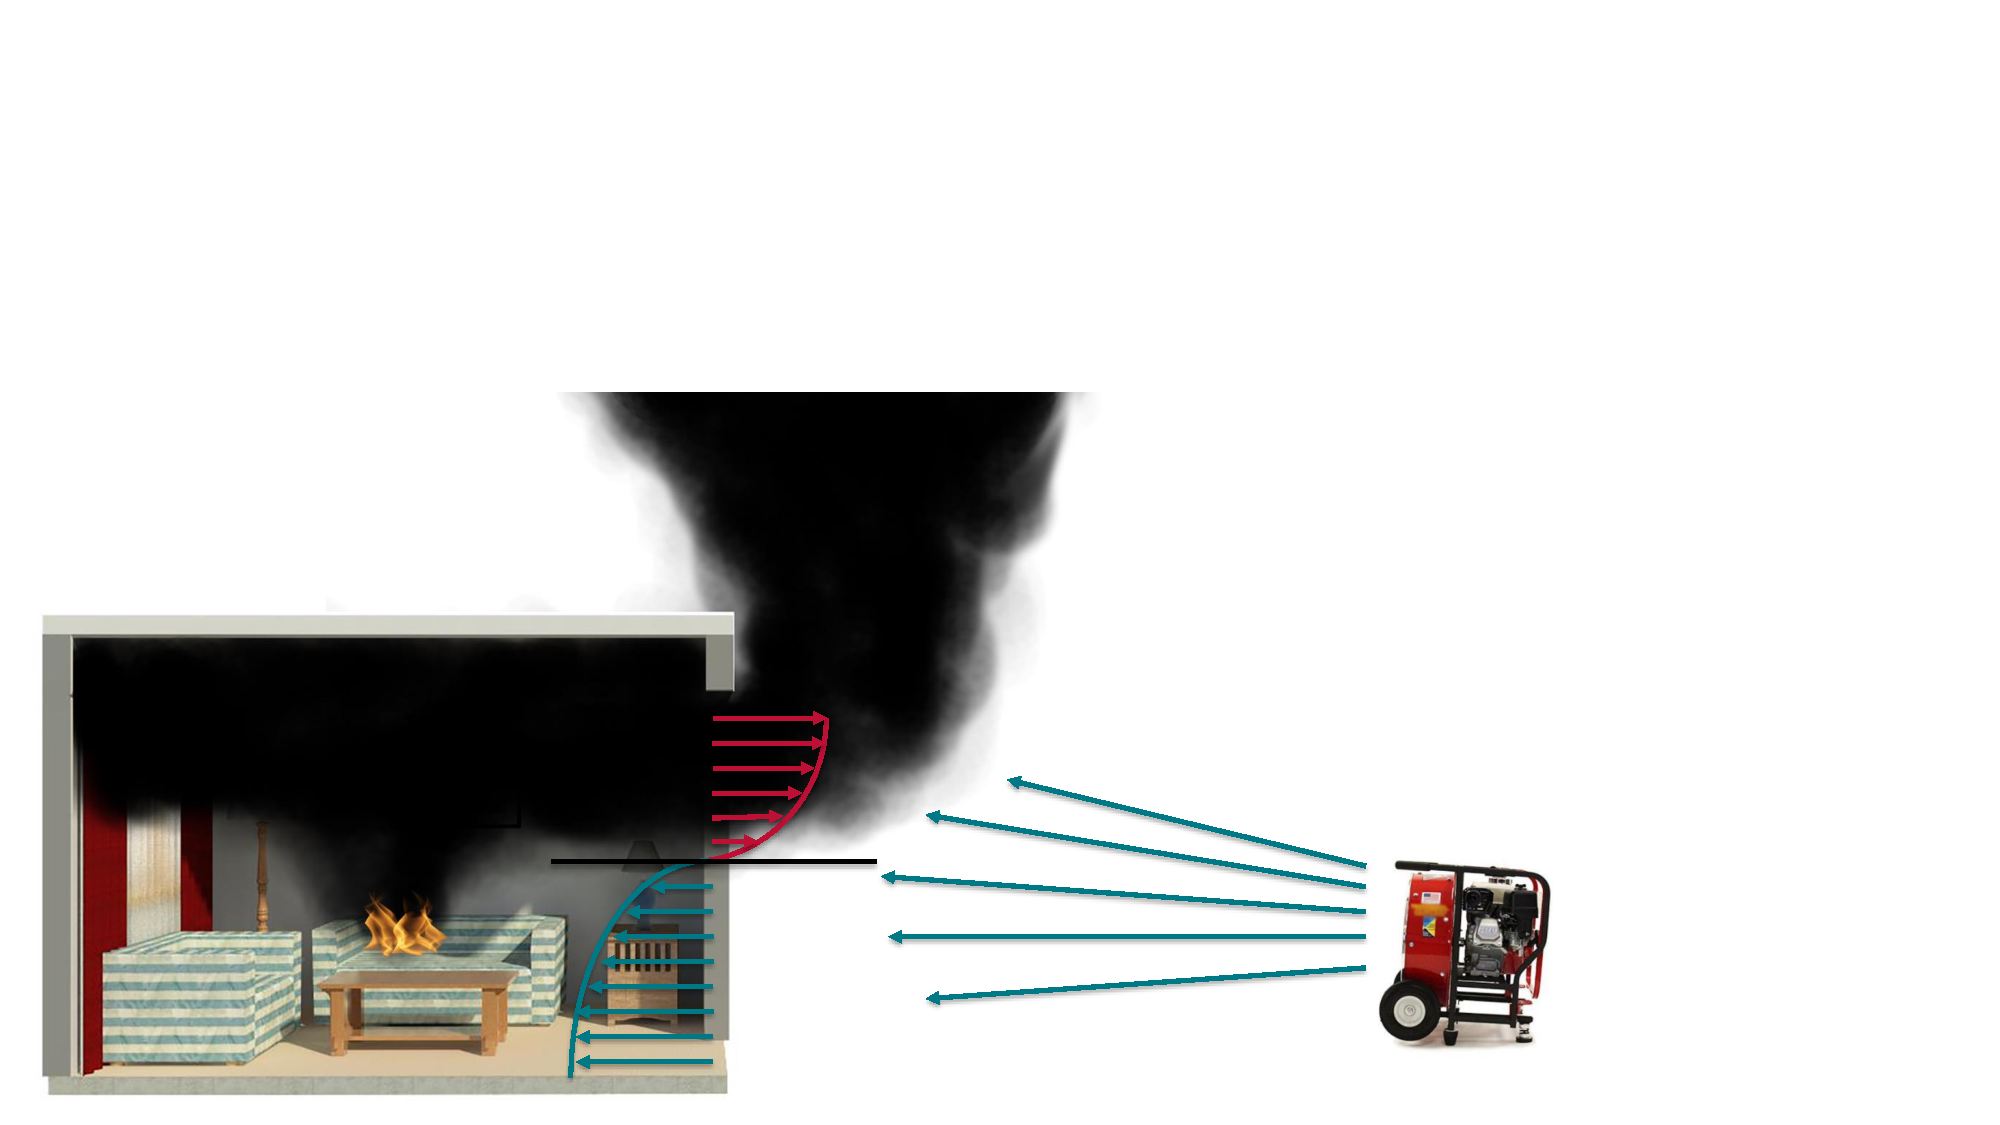
\includegraphics[width = 6in]{0_Images/Tactical_Considerations/Ongoing_Assessment/FanandDoorFlow.pdf}
	\caption{Inlet Flows During Positive Pressure Attack}
	\label{fig:FanAndDoorFlow}
\end{figure}

The pressure in the structure is greater than the outside pressure. This, combined with the non-uniform pressure from the fan, will result in back flow from the top of the doorway. Figure \ref{fig:DoorVelocity} illustrates the front door flow once steady state had been reached for each ventilation configuration tested in the single story and two story structures. The center line is zero flow, any values to the right of the center are outflow, and any values to the left of the line are inflow. Regardless of the exhaust size or location, back flow was always seen at the inlet.

\begin{figure}[H]
	\centering
	\begin{tabular}{c c}
		\subfloat[Single Story]{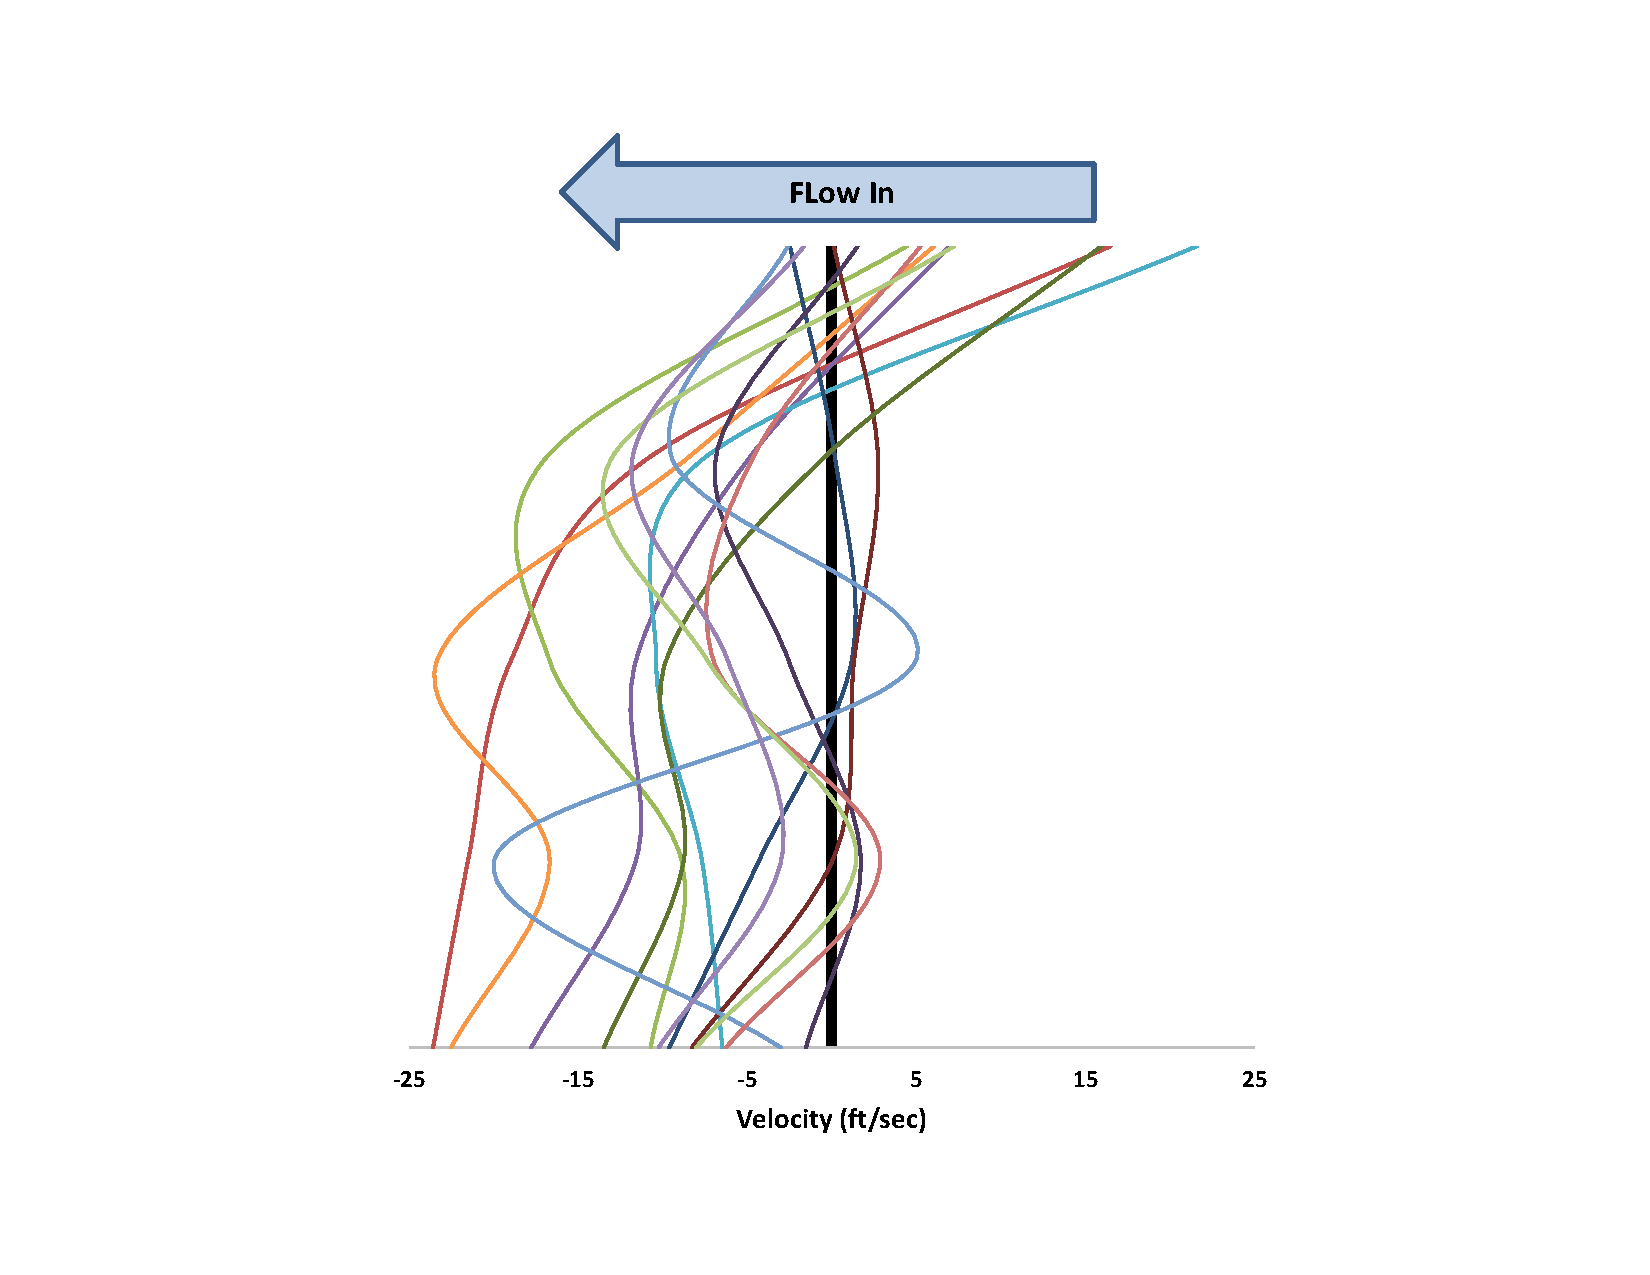
\includegraphics[width = 2.5in]{0_Images/Tactical_Considerations/Ongoing_Assessment/SingleStoryFrontDoorVelocities.pdf}} &
		\subfloat[Two Story]{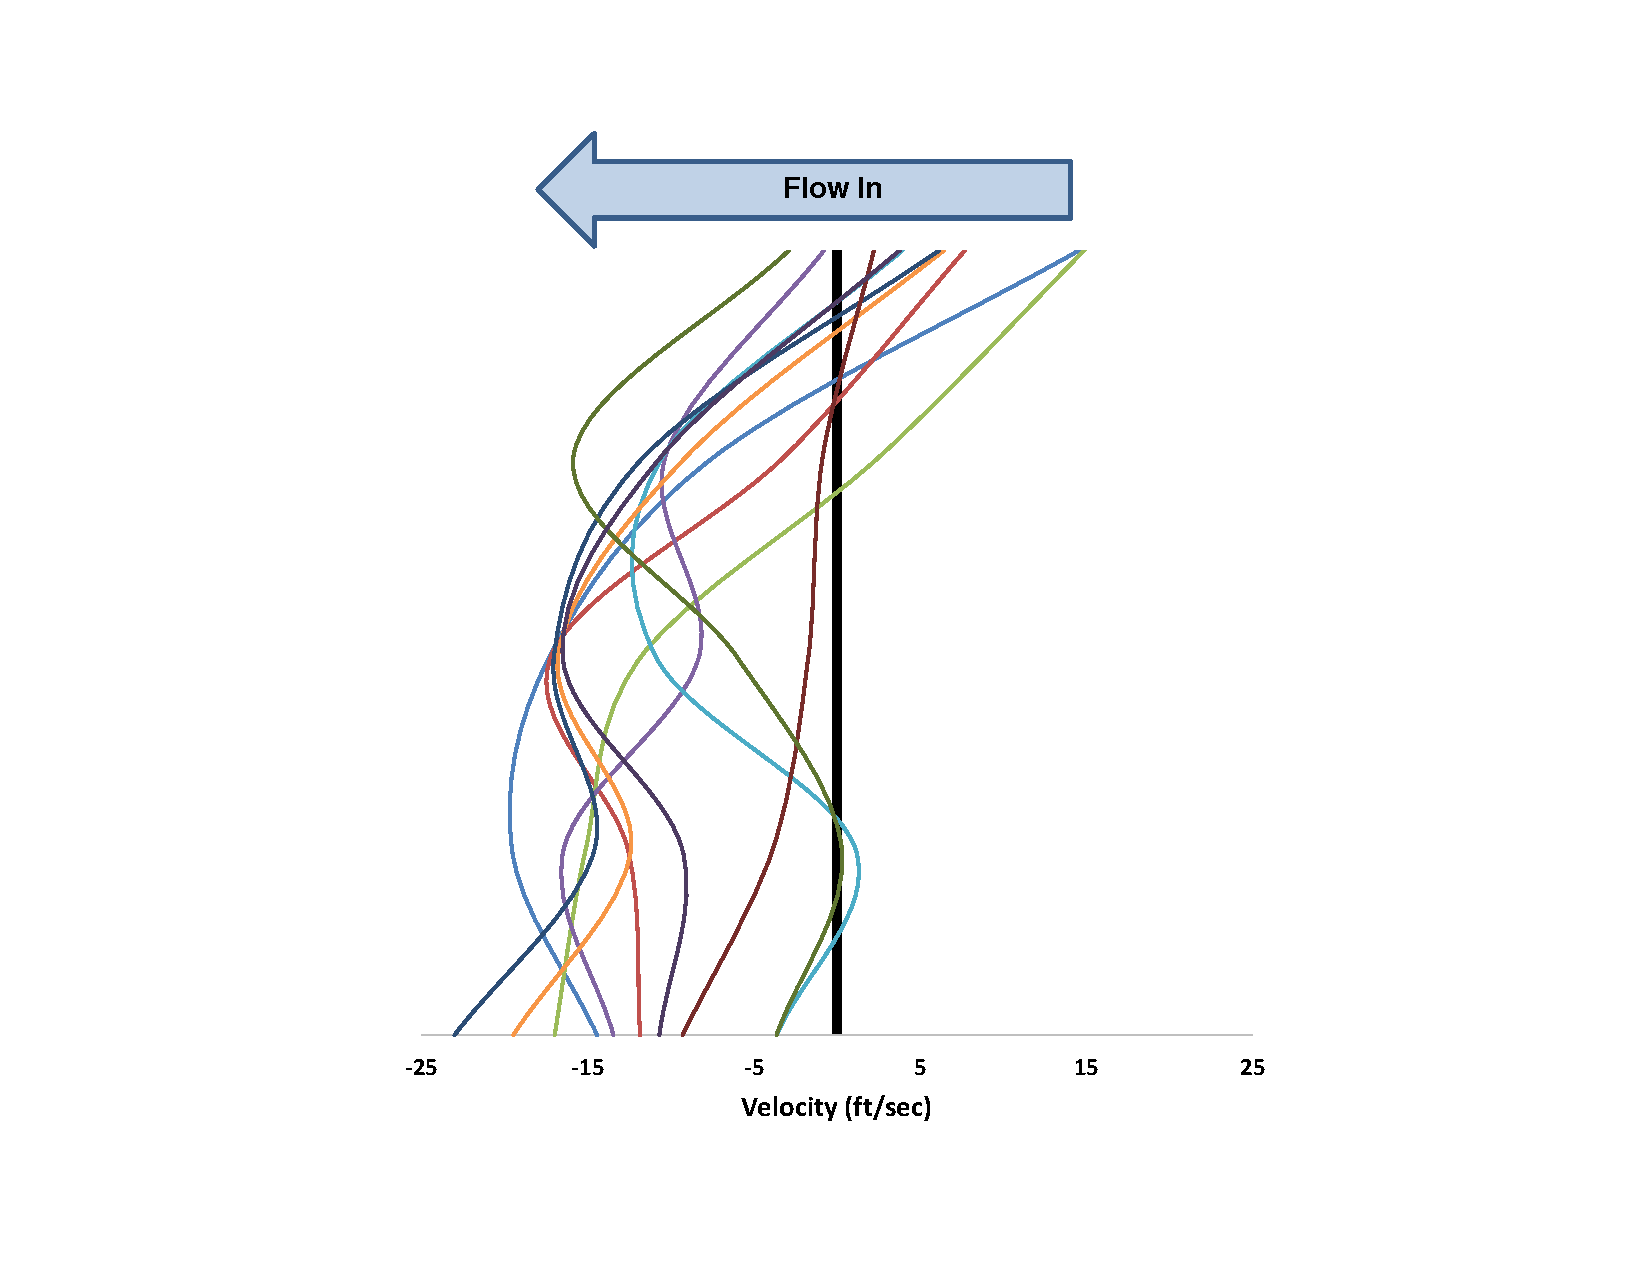
\includegraphics[width = 2.5in]{0_Images/Tactical_Considerations/Ongoing_Assessment/TwoStoryFrontDoorVelocities.pdf}} \\
	\end{tabular}
	\caption{Front Door Velocity}
	\label{fig:DoorVelocity}
\end{figure}

If the fire is producing a low HRR because it has decayed due to lack of oxygen or is a small fire, such as a trash can or food on the stove, you can get what appears to be flow through the whole doorway. With no smoke in the space, the periodic exhaust seen at the top of the door during ventilation limited fires is not visible. The experiments conducted for this project were room fires with the potential for flashover conditions. These fires built up smoke in the entire structure, which resulted in the visual flow out the top of the door.  

Although backflow at the front door does not indicate the effectiveness of PPA, several other indicators were observed. At the inlet, flow out of the top of the door was observed immediately after the door is opened. This is the smoke which has been confined to the compartment in which the inlet is located. Once PPA is initiated, if the exhaust is effective, over time this smoke will decrease in volume. Increased smoke volume or darkening color at the attack entrance may indicate that there is too little exhaust. Use both the neutral plane at the attack entrance and at the exhaust to identify progress. A descending neutral plane at the front door indicates the flow moving towards the fan is increasing, potentially indicating the fire is extending or spreading out of the initial fire compartment.

\begin{figure}[H]
	\centering
	\begin{tabular}{c c c}
		\subfloat[Door Open]{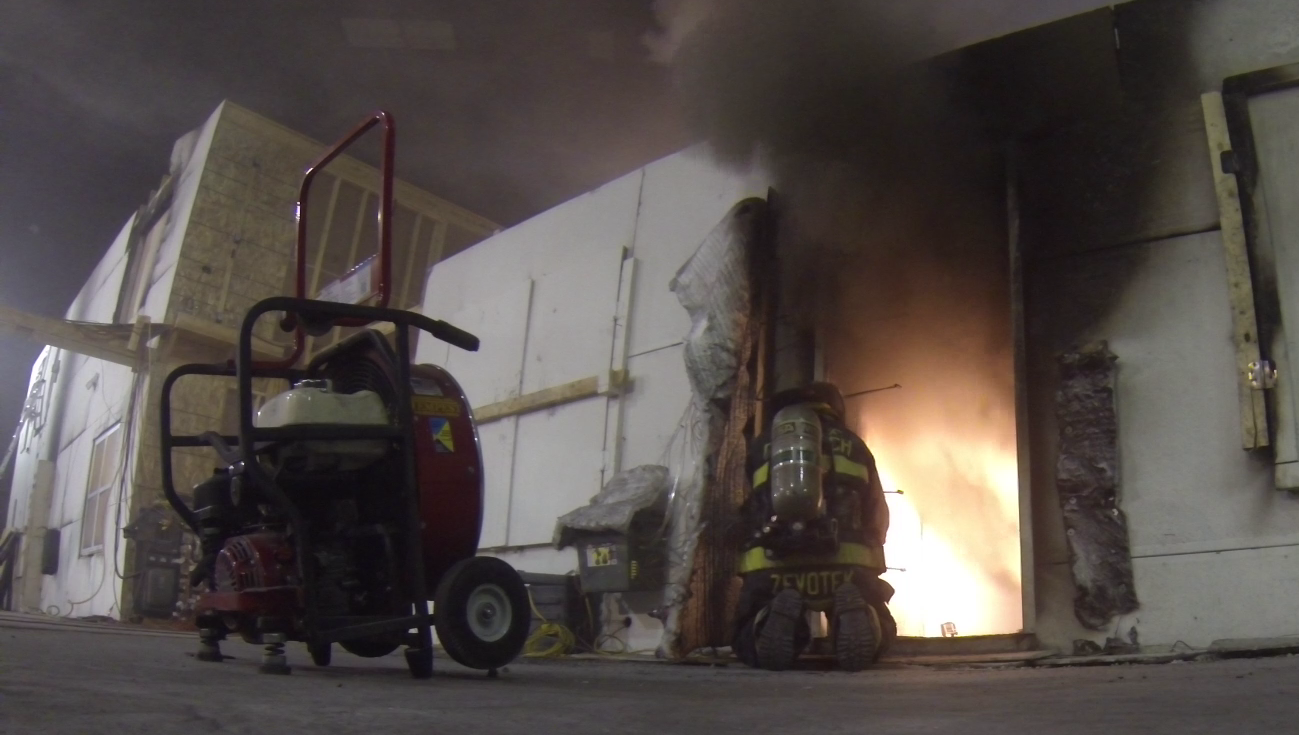
\includegraphics[width = 1.5in]{0_Images/Tactical_Considerations/Ongoing_Assessment/ReadInlet/Open.png}} &
		\subfloat[Fan On]{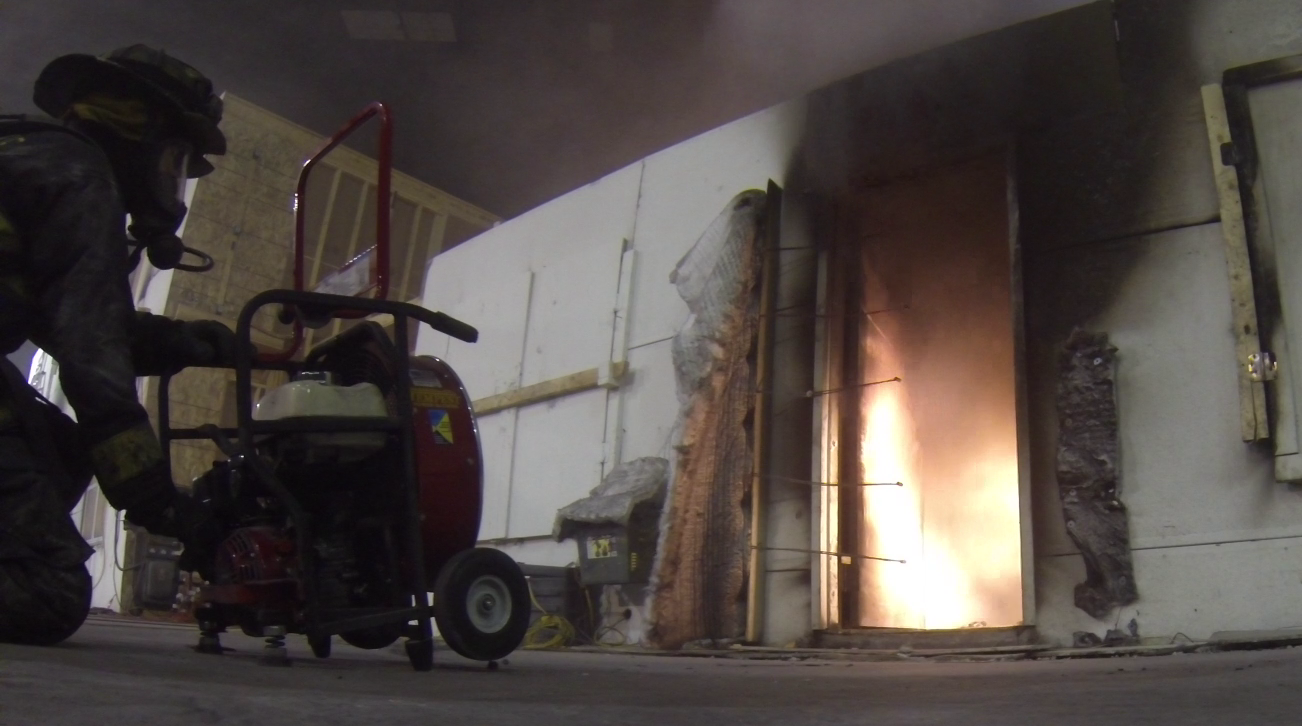
\includegraphics[width = 1.5in]{0_Images/Tactical_Considerations/Ongoing_Assessment/ReadInlet/FanOn.png}} &
		\subfloat[30 Seconds]{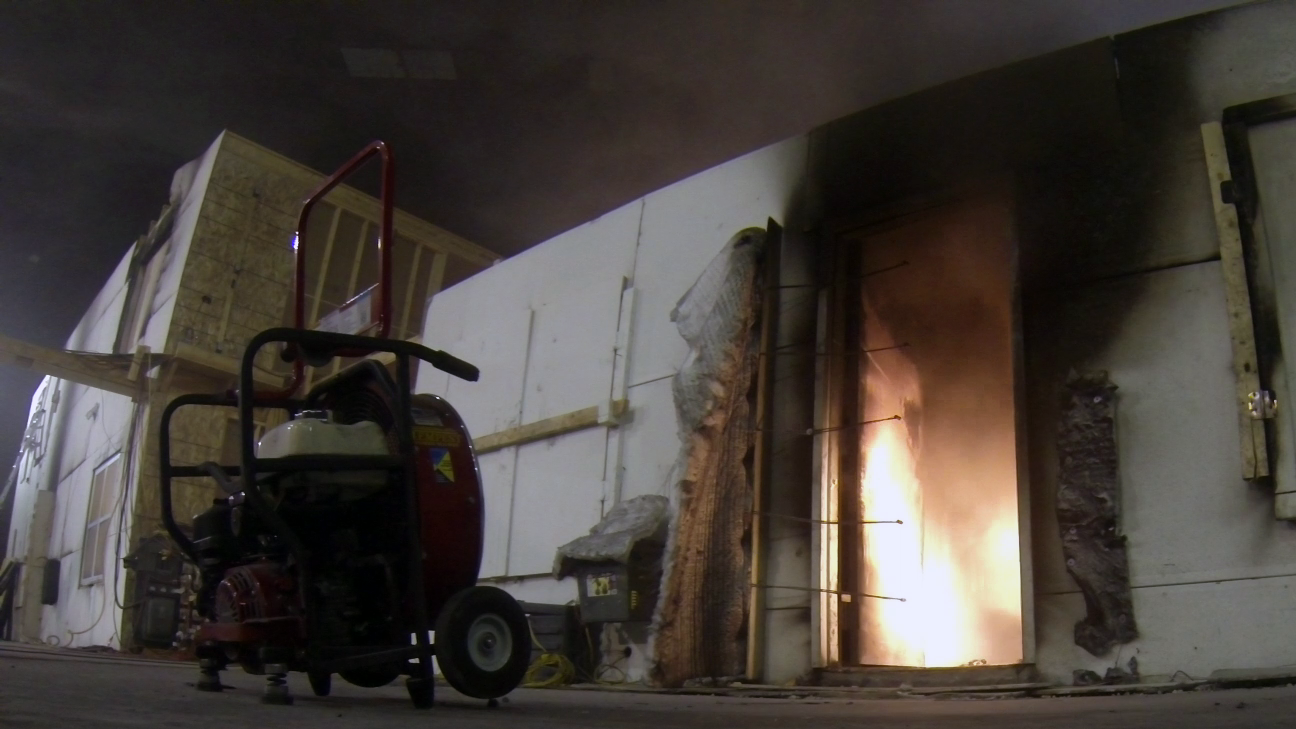
\includegraphics[width = 1.5in]{0_Images/Tactical_Considerations/Ongoing_Assessment/ReadInlet/30Sec.png}} \\
		\subfloat[60 Seconds]{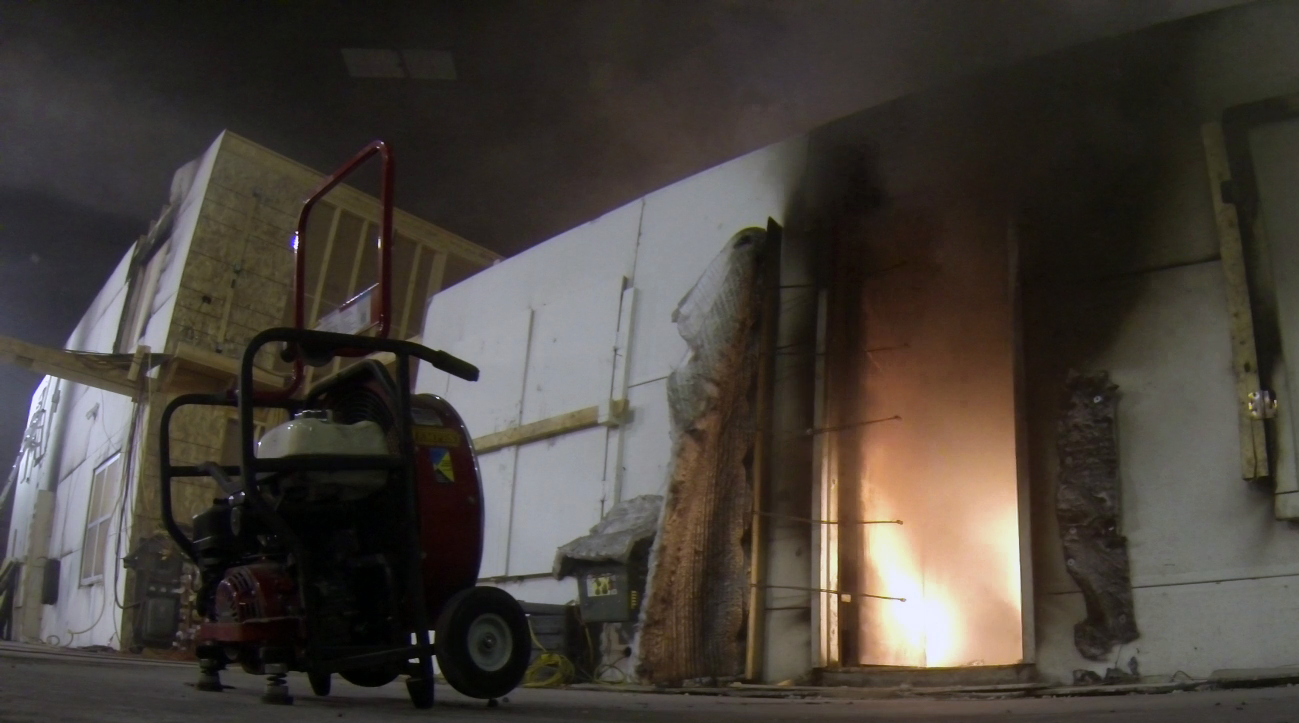
\includegraphics[width = 1.5in]{0_Images/Tactical_Considerations/Ongoing_Assessment/ReadInlet/60Sec.png}} &
		\subfloat[90 Seconds]{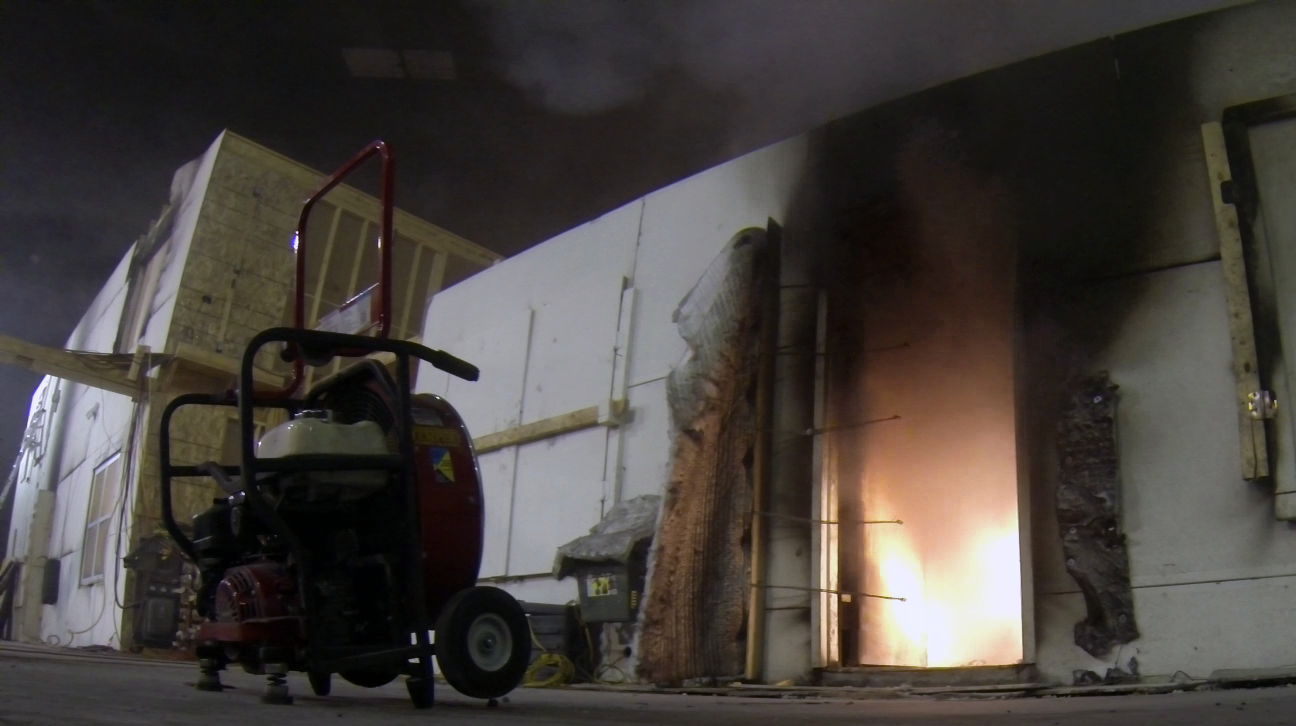
\includegraphics[width = 1.5in]{0_Images/Tactical_Considerations/Ongoing_Assessment/ReadInlet/90Sec.png}} &
		\subfloat[120 Seconds]{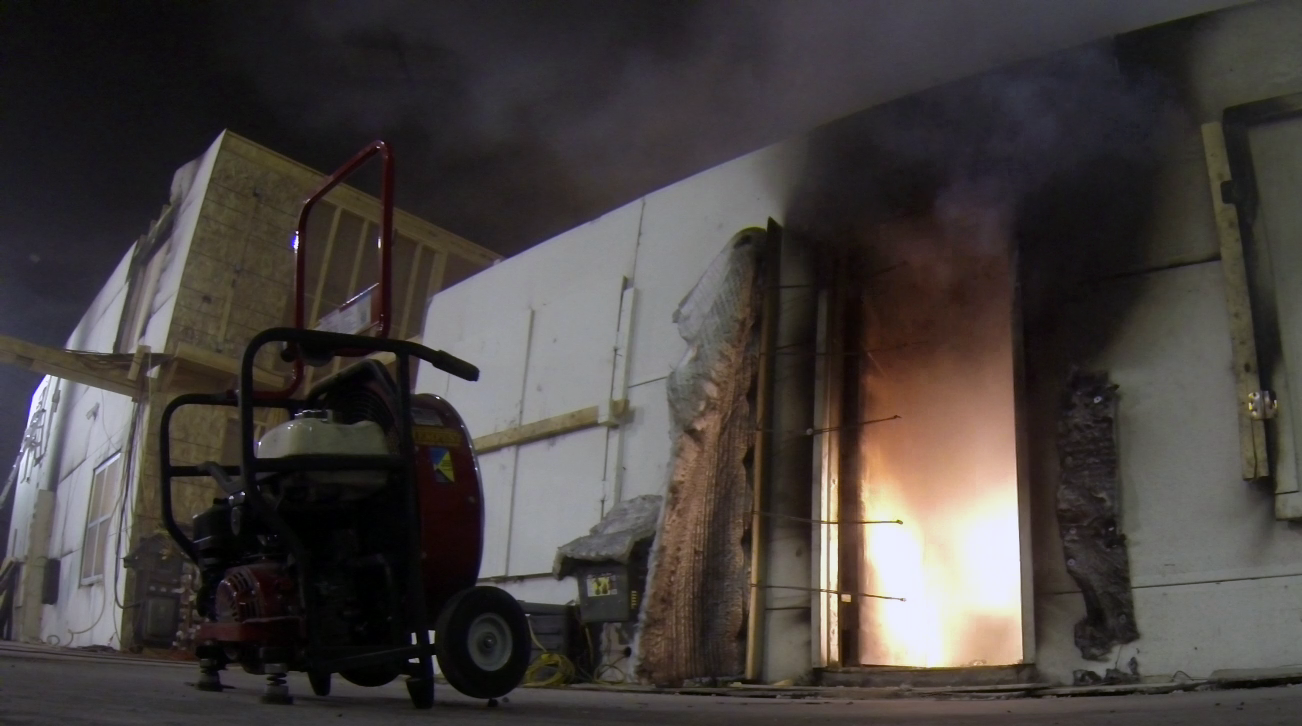
\includegraphics[width = 1.5in]{0_Images/Tactical_Considerations/Ongoing_Assessment/ReadInlet/120Sec.png}} \\
		\subfloat[150 Seconds]{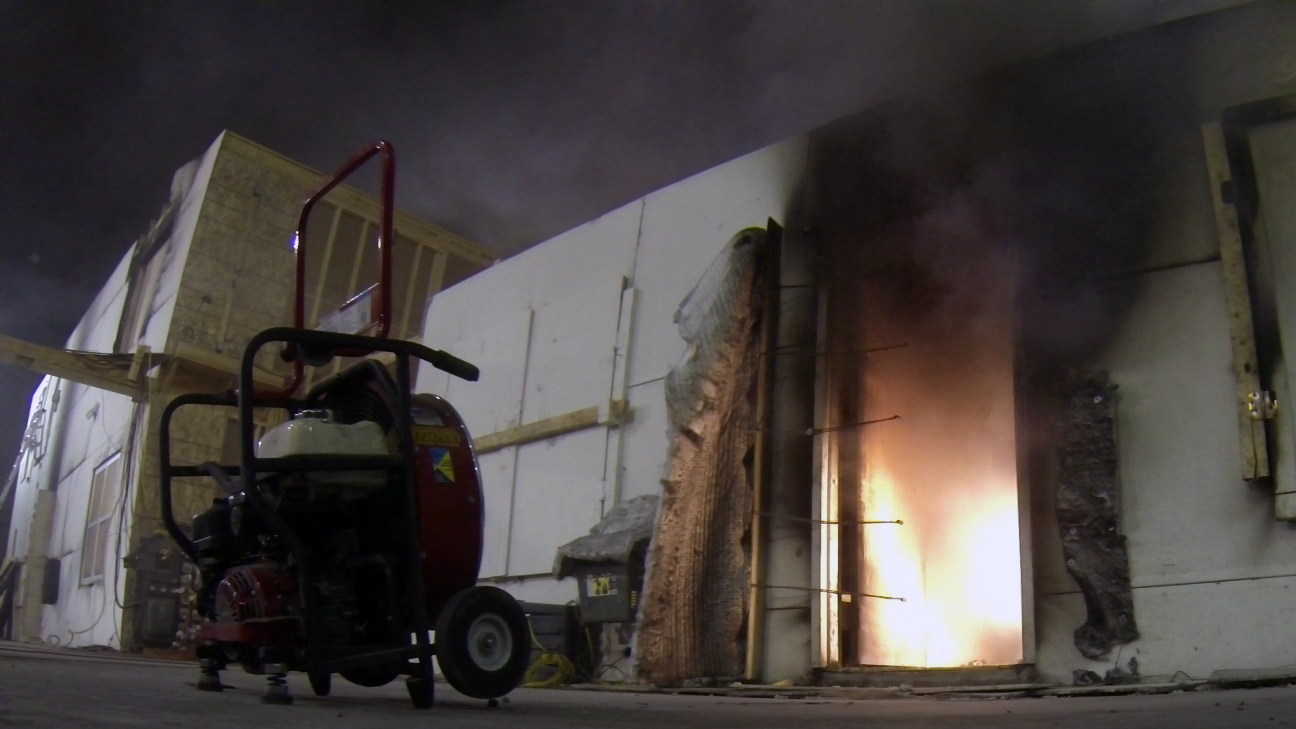
\includegraphics[width = 1.5in]{0_Images/Tactical_Considerations/Ongoing_Assessment/ReadInlet/150Sec.png}} &
		\subfloat[180 Seconds]{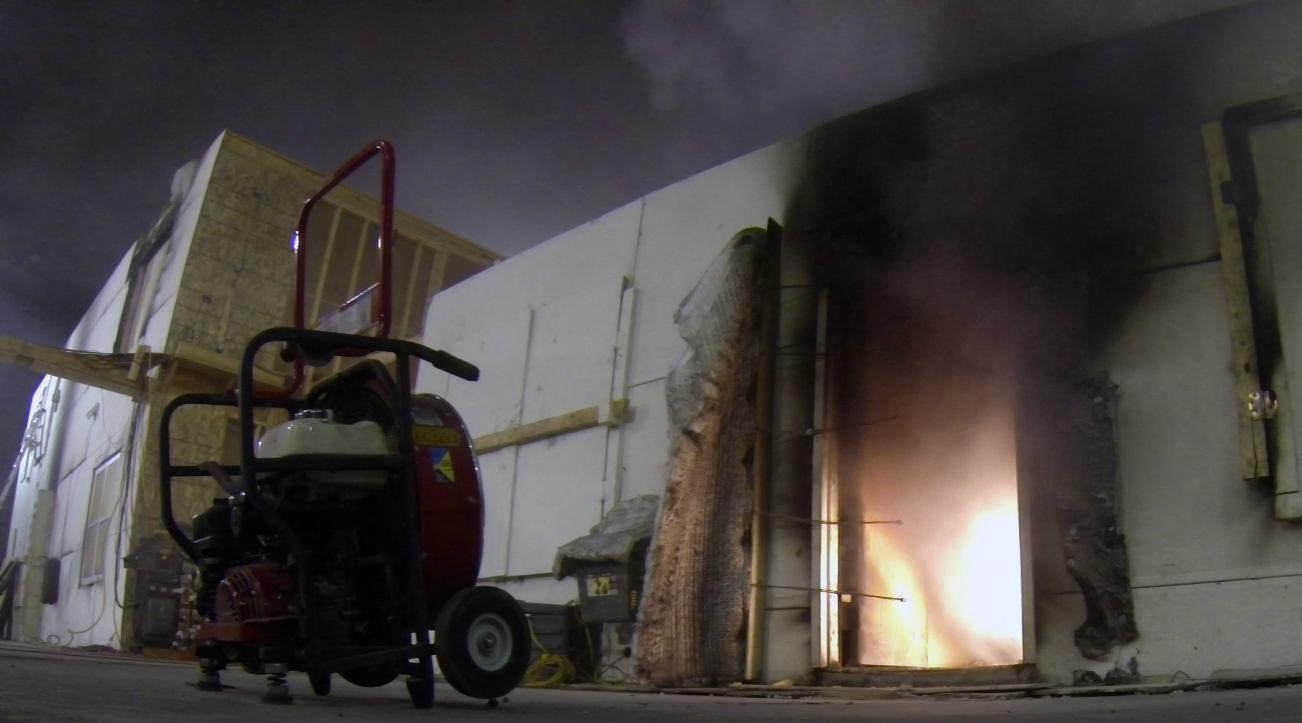
\includegraphics[width = 1.5in]{0_Images/Tactical_Considerations/Ongoing_Assessment/ReadInlet/180Sec.png}} &
		\subfloat[210 Seconds]{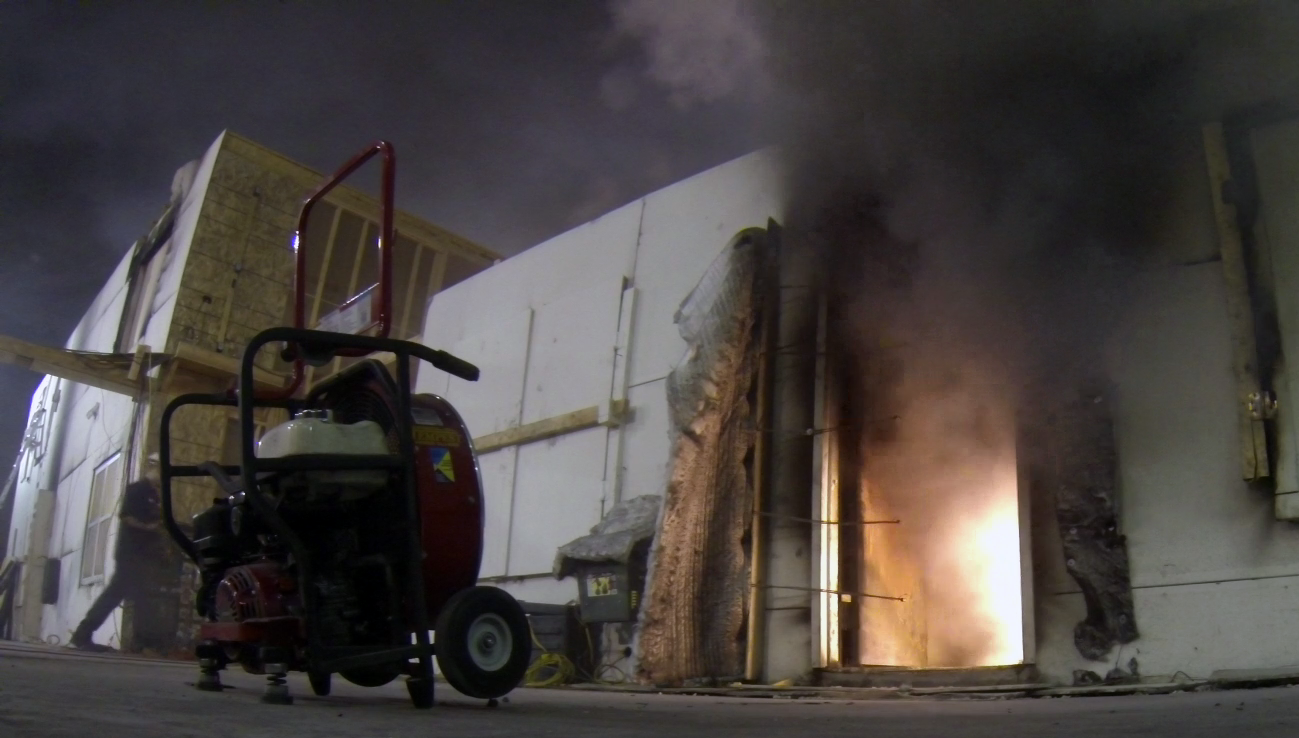
\includegraphics[width = 1.5in]{0_Images/Tactical_Considerations/Ongoing_Assessment/ReadInlet/210Sec.png}} \\
	\end{tabular}
	\caption{Reading the Inlet}
	\label{fig:ReadingInlet}
\end{figure}

When assessing the exhaust locations (s), the impact of PPA will be noticeable within seconds (Figure \ref{fig:ReadExhaust}). When the exhaust is first created the buoyant flows will result in a neutral plane located somewhere in the window depending on the location of the fire and stage of fire growth. The high pressure hot gases (smoke) will flow out the top of the window above the neutral plane. A gravity flow of cooler ambient air will flow in the bottom, below the neutral plane. Once the fan is turned on, the neutral plane should drop to the windowsill and the exhaust should become a unidirectional flow indicating the fan flow path has been established. A neutral plane above the window sill on the exhaust opening while conducting PPA indicates more flow is required or an obstruction exists between the inlet and the exhaust. This indicates additional actions such as increasing the fan flow by adding a fan or increasing fan throttle are necessary while ensuring the no obstruction exists in the intended fan flow path. If increased exhaust vent flow cannot be established within a short period of time, crews should stop the fan and consider implementing a different tactic.

\begin{figure}[H]
	\centering
	\begin{tabular}{c c c}
		\subfloat[Exhaust Without Fan Flow - Pre Flashover]{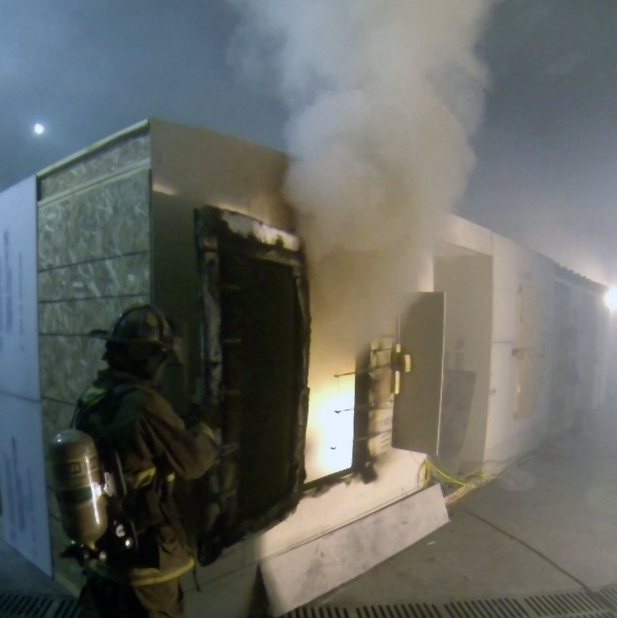
\includegraphics[width = 2.25in]{0_Images/Tactical_Considerations/Ongoing_Assessment/ReadExhaust/NoFanSmoke.png}} &
		\subfloat[Exhaust With Fan Flow - Pre Flashover]{\includegraphics[width = 2.25in]{0_Images/Tactical_Considerations/Ongoing_Assessment/ReadExhaust/FanSmoke.png}} \\
		\subfloat[Exhaust Without Fan Flow - Post Flashover]{\includegraphics[width = 2.25in]{0_Images/Tactical_Considerations/Ongoing_Assessment/ReadExhaust/NoFanFire.png}} &
		\subfloat[Exhaust With Fan Flow - Post Flashover]{\includegraphics[width = 2.25in]{0_Images/Tactical_Considerations/Ongoing_Assessment/ReadExhaust/FanFire.png}} \\
	\end{tabular}
	\caption{Reading the Exhaust}
	\label{fig:ReadExhaust}
\end{figure}

In addition to monitoring exterior conditions, interior crews must be monitoring interior conditions. Ineffective PPA has the potential to cause conditions to deteriorate faster than would be noted in horizontal or vertical ventilation. Identifying and reacting to deteriorating conditions becomes even more essential during PPA. With the fan introduced, interior crews should notice a decrease in temperature and increased visibility over time. If this is not the case, the structure should be evacuated until the elements required for a successful PPA are re-evaluated.

\subsection{Positive Pressure Attack is Exhaust Dependant} \label{sec:ExhaustDepend}
For PPA to be effective the pressure created by the fan must be greater than the pressure created by the fire. Although fan size does play a role in the effectiveness of PPA, exhaust size plays a greater role. Providing enough exhaust to reduce the pressure in the fire room to a pressure below what the fan is capable of producing in the remainder of the structure is essential for safe PPA operations.

A fire in post flashover state, venting to the exterior was seen to produce between 9Pa and 11Pa of pressure in the upper layer 1ft from the ceiling. This means for the fan to prevent flow from the fire compartment to an adjacent compartment, the adjacent compartment needs to be at least 9Pa, preferably 11Pa or higher. 

\begin{table} [H]
	\centering
	\caption{Venting - Post Flashover Fire Room Pressure Increase}
	\centering
	
	\begin{tabular}{|c|c|c|}
		\hline
		Experiment Number & $\delta$ Pressure (Pa) & Time Period (Min) \\ \hline \hline
		6 & 11.10 & 7:40 - 8:00 \\ \hline
		8 & 9.64 & 8:50 - 9:08 \\ \hline
		9 & 10.56 & 8:00 - 8:40 \\ \hline
		10 & 10.62 & 6:20 - 6:35 \\ \hline
		11 & 10.71 & 7:55 - 8:10 \\ \hline
		12 & 11.27 & 7:30 - 8:00 \\ \hline
		Average & 10.65 & -  \\ \hline
	\end{tabular}
	
	\begin{tablenotes}
		\centering
		\item Note: Only experiments where post flashover fire venting \\ to the exterior, prior to starting the fan \\ were utilized in this analysis.
	\end{tablenotes}
	\label{tab:FireRoomPressure}
\end{table}

With the intent of PPA to direct the flow out of the exhaust vent rather than into the structure, creating the pressure differential is imperative. The greater the differential pressure between the fire room and adjacent spaces, the more effective the PPA will be at keeping fire gases out of the adjacent spaces.

The most effective way to ensure that the pressure from the PPA in the adjacent compartments is higher than the pressure in the fire room is to have the exhaust openings in the fire room be larger than the inlet of the opening to the fire room.  For this reason, PPA/PPV training has placed a great deal of emphasis on the ideal exhaust to inlet ratio for PPA. The inlet size was thought to be the opening where the fan was placed. However, the true inlet is the opening to the fire compartment. In the structures tested, the interior doors had 16.7$ft^2$ of opening area and the entrance door had 20$ft^2$ of opening area. It should be noted that in most structures, the front door size is slightly larger than interior doors, however not vastly different sizes, thus the front door can be used as an approximation of the interior door size.

The experiments found PPA most effective when the fire was in a compartment separated from the remainder of the structure (see tactical consideration \ref{OpenSpaces}). Figure \ref{fig:RanchStructureOpenings} illustrates the opening sizes and intended fan flow for several of the experiments conducted. In the structures tested, the bedrooms had windows with 15$ft^2$ of opening area per window, with either one or two windows per bedroom. The bedroom door opening of 16.7$ft^2$ provided a limiting point for the flow, making the pressure in the living room and hallway higher than the pressure in the bedroom when the 15$ft^2$ window was open. However, because the window opening was smaller than the bedroom door the amount of flow exhausting the bedroom window was less than what was entering the bedroom door making the window the most limiting. This resulted in a pressure increase in the bedroom. 

In order to create the intended fan flow, the pressure in the fire room must be lower than the pressure in adjacent spaces. As seen in Figure \ref{fig:OneVSTwoWindowsColdFlow}, under cold flow conditions, when positive pressure attack is utilized the entire volume of the house is more or less at the same pressure, with the exception of the room where the exhaust is provided (bedroom 2). The lower pressure in the bedroom creates a flow from the higher pressure adjacent spaces into the lower pressure bedroom and out the low pressure vent. When the single window was open providing an exhaust to inlet ratio of approximately 1:1, the pressure in the exhaust room (bedroom 2) was 1/2 the pressure of the living room. Once the second window as open, the door to the bedroom became the limiting factor for flow in, resulting in no pressure increase in the bedroom.

\begin{figure}[H]
	\centering
	\includegraphics[width = 4in]{0_Images/Tactical_Considerations/PPA_Exhaust_Dependant/Opening_Sizes.pdf}
	\caption{Opening Sizes - Single Story Ranch Structure}
	\label{fig:RanchStructureOpenings}
\end{figure}

With this principle in mind, any exhaust to inlet ratio greater than 1:1 will not result in a pressure rise in the fire compartment due to the fan, only what the fire is capable of producing. In the configuration shown, as long as the fan is capable of creating greater than 11Pa of pressure in adjacent spaces, all of the products of combustion being created in the bedroom will exhaust out the bedroom windows. 

\begin{figure}[H]
	\centering
	\begin{tabular}{c c}
		\subfloat[Differential Pressures Within the Structure]{\includegraphics[width = 3.5in]{0_Images/Tactical_Considerations/An_Outlet_Must_be_Provided/Bedroom2SingleVDoubleWindow.pdf}} & 
		\subfloat[Ventilation Configuration]{\includegraphics[width = 1.75in]{0_Images/Tactical_Considerations/An_Outlet_Must_be_Provided/DoubleWindowBed2.pdf}} \\
	\end{tabular}
	\caption{Single Window vs. Double Window Cold Flow Pressure}
	\label{fig:OneVSTwoWindowsColdFlow}
\end{figure}

This also applies under fire conditions. If not enough exhaust is provided, the pressure created by the fire and the fan, will overwhelm the pressure created by the fan causing the the fire to grow back towards the fan. The solution is to lower the pressure in the fire compartment by 1) creating more exhaust openings in the fire compartment or 2) applying water to reduce the pressure created by the fire. 

Testing demonstrated a 2:1 exhaust to inlet ratio was much more effective than a ration of 1:1 or less. Although under non-fire conditions, the pressure in the bedroom with one window open is less than in the remainder of the structure, when fire is introduced it creates additional pressure. As the heat release rate of the fire increases, the pressure in the fire room increases. At the point where the fire room pressure matches the remainder of the structure, combustion products will flow from the fire room into the structure again. This increases temperatures, and transfers smoke and toxic gases from the fire compartment to the remainder of the structure. Figure \ref{fig:SingleVsDoubleWindow}b illustrates the increasing pressure as the fire grows (bedroom 2). At 10:15, when the pressure in the fire room (bedroom 2) is equal to the adjacent spaces, hot gas flow exits the top of the bedroom 2 door and flows back into the hall as seen in  Figure \ref{fig:SingleVsDoubleWindow}a. Creating the additional exhaust openings in the fire compartment and reaching a 2:1 ratio of exhaust to inlet results in a decrease of pressure in the fire room and the products of combustion are all exhausted. 

An additional means of reducing the pressure in the fire compartment would be through the application of water. Applying water to the fire reduces the heat release rate of the fire, and thus the pressure it can produce. If the fire is not adding pressure to the pressure created by the fan, the pressure difference between the fire compartment and adjacent spaces created by the fan with one exhaust will direct the flow out the exhaust opening rather than back into the structure. 

\begin{figure}[H]
	\centering
	\begin{tabular}{c c}
		\subfloat[Bedroom 2 Door Flow]{\includegraphics[width = 3.0in]{0_Images/Tactical_Considerations/An_Outlet_Must_be_Provided/FlowOneVTwoVents.pdf}} &
		\subfloat[Pressure Throughout Structure]{\includegraphics[width = 3.in]{0_Images/Tactical_Considerations/An_Outlet_Must_be_Provided/PressOneVTwoVents.pdf}} \\
	\end{tabular}
	\subfloat[Ventilation Configuration]{\includegraphics[width = 2.5in]{0_Images/Tactical_Considerations/An_Outlet_Must_be_Provided/Exp3VentConfigurations.pdf}}
	\caption{Positive Pressure Attack - Single Window Vs Double Window Fire}
	\label{fig:SingleVsDoubleWindow}
\end{figure}

Earlier research by NIST involved the impact of wind on positive pressure effectiveness. The work concluded positive pressure fans alone are not capable of overcoming the pressure created by the opposing wind condition. An exhaust on the windward side (high pressure side) of the structure will create a hazardous situation and should be avoided. If no other exhaust option is available firefighters should consider another tactic \cite{KerberMadrzyPPVInHighRise}. 

Proper exhaust size will limit the flow of heat and smoke from the fire compartment to the remainder of the structure. Heat and smoke flowing from the fire room towards the fan has the potential to cause vent point ignition at the fan inlet as seen in Figure \ref{fig:VentPointIgnitionLab} and \ref{fig:VentPointIgnitionField}. This is a very dangerous situation for fire fighters, as it indicates untenable conditions within the intended fan flow path, potentially cutting off the primary means of egress for the attack team.

\begin{figure}[H]
	\centering
	\includegraphics[width = 5in]{0_Images/Tactical_Considerations/PPA_Exhaust_Dependant/Vent_Point_Ignition.png}
	\caption{Vent Point Ignition of Fan Inlet During Laboratory Experiments}
	\label{fig:VentPointIgnitionLab}
\end{figure}

\begin{figure}[H]
	\centering
	\includegraphics[width = 5in]{0_Images/Tactical_Considerations/PPA_Exhaust_Dependant/Vent_Point_Ignition_Field.png}
	\caption{Vent Point Ignition of Fan Inlet From Incident Video}
	\label{fig:VentPointIgnitionField}
\end{figure}

Providing additional exhaust in the fire room will not negatively affect positive pressure attack, as it can only aid in ensuring the pressure created from the fire is not able to build and overcome the pressure created by the fan. With the size of a single window often being less square footage than the size of the door to the room, it will be necessary to vent additional windows to achieve the greater than a ratio of 1:1. 

Many rooms only have one window, or the sum of the area the windows in the room is less than the area of the door to the room. This does not mean the tactic of positive pressure attack will be ineffective, just that it will be less effective. An effort should be made to ensure the maximum exhaust ratio is achieved with all exhaust locations being in the fire room. If a minimum of a 1:1 ratio cannot be achieved, firefighters should consider a tactic other than PPA. 

Even when the required pressure difference is achieved between the fire room and adjacent spaces, backflow at the inlet where the fan is located will still occur. See tactical consideration \ref{sec:OngoingAssessment} for a description of why backflow at the inlet is not an indicator of what flows are occurring within the structure and alone cannot identify the effectiveness of a positive pressure attack.

\subsection{An outlet of sufficient size, must be provided, in the fire room to allow for effective PPA.} \label{sec:OutletInFireRoom}
PPA effectiveness is directly dependent on the ability of the fan to exhaust products of combustion to the exterior. Any exhaust opening created in conjunction with PPA should be located in the fire compartment. Exhaust openings not provided in the fire compartment will create unintended flow paths, resulting in the spread of smoke, and potentially fire into the room in which the exhaust is made. For example, as shown in Figure \ref{fig:ExhaustLocationComp}, when a vent is opened in the fire room, most of the heat and smoke will be vented out the window resulting in temperatures remaining low in the adjacent rooms. When the exhaust vent is created in an adjacent room, it results in temperature increase in that room.

\begin{figure}[H]
	\centering
	\begin{tabular}{c c}
		\setcounter{subfigure}{0} 
		\subfloat[5ft Temperature in Adjcent Bedrooms \& Hallway Comparison]{\includegraphics[width = 3.75in]{0_Images/Tactical_Considerations/An_Outlet_Must_be_Provided/VentComparisonTemps.pdf}} & 
		\subfloat[Ventilation Profile - Adjacent vs Fire Room Vent]{\includegraphics[width = 1.75in]{0_Images/Tactical_Considerations/An_Outlet_Must_be_Provided/ExhaustLocationLayoutFire.pdf}} \\
	\end{tabular}
	\caption{Exhaust Location Comparison with Fire in Bedroom 3}
	\label{fig:ExhaustLocationComp}
\end{figure}

Not only is the location of the exhaust important, but also the area or size of the opening. Even when an exhaust opening is located in the fire compartment, if it is not of sufficient size, the effect will be similar to exhaust in an adjacent compartment. The pressure created by the fire, combined with the pressure increase in the room due to the fan, will exceed the pressure created by the fan in the adjacent space, resulting in flow from the fire compartment into adjacent compartments. This results in increased temperatures, decreased visibility, and decreased survivability as discussed in tactical consideration \ref{sec:ExhaustDepend}.

\begin{figure}[H]
	\centering
	\begin{tabular}{*2c}
		\subfloat[Heat Flux from Window at 8ft]{\includegraphics[width = 3in]{0_Images/Tactical_Considerations/PPA_Exhaust_Dependant/Experiment8-HeatFlux.pdf}} &
		\subfloat[Heat Flux from Window at 12ft]{\includegraphics[width = 3in]{0_Images/Tactical_Considerations/PPA_Exhaust_Dependant/Experiment6-HeatFlux.pdf}} \\
	\end{tabular}
	\caption{Heat Flux from Bedroom 2 Window Vent}
	\label{fig:HeatFluxVent}
\end{figure}

As with any ventilation tactic, extension to exposures needs to be a consideration when utilizing PPA. The use of the fan intensifies the volume of fire venting from the exhaust window. As seen in Figure \ref{fig:HeatFluxVent} shows the energy received at 8ft away increases by almost 300\% once the fan is introduced. At 12ft the increase is over 150\%. Any exhaust created during PPA should be coordinated to limit the exposure potential. 


\subsection{During PPA, creating additional openings not in the fire room will create additional flow paths making PPA ineffective with the potential to draw the fire into all flow paths}
Additional openings not in the fire compartment will lower the pressure in the adjacent compartments, allowing for more flow from the fire compartment to the remainder of the structure. An example of this would be ventilating all of the bedroom windows in a ranch home prior to implementing positive pressure attack (Figure \ref{fig:AdditionalVents_Configurations}). 

\begin{figure} [H]
	\centering
	\begin{tabular}{*2c}
		\subfloat[Configuration - Single Vent]{\includegraphics[width = 3.25in]{0_Images/Tactical_Considerations/Additional_Vent/SingleVent.png}} &
		\subfloat[Configuration - Multiple Vents]{\includegraphics[width = 3.25in]{0_Images/Tactical_Considerations/Additional_Vent/Multiple_Vents.png}} \\
	\end{tabular}
	\caption{Additional Ventilation Outside the Fire Compartment}
	\label{fig:AdditionalVents_Configurations}
\end{figure}

\begin{figure} [H]
	\centering
	\includegraphics[width = 3 in]{0_Images/Tactical_Considerations/Additional_Vent/PressureSingle_Multiple.pdf}
	\caption{Additional Ventilation Openings Reduce Pressure Created by Fan}
	\label{fig:AdditionalVents_Pressure}
\end{figure}

With four times the additional ventilation openings, the fan cannot maintain the same amount of pressure in the living room. Figure \ref{fig:AdditionalVents_Pressure} shows the fan produced only approximately 1/2 the pressure increase when four times the ventilation openings were provided. The reduction in pressure in the living room resulted in additional fire gas flow from the fire room to surrounding compartments. 

\begin{figure} [H]
	\centering
	\begin{tabular}{*2c}
		\subfloat[Door Flow Bedroom 2 Door - Single Vent]{\includegraphics[width = 3.25in]{0_Images/Tactical_Considerations/Additional_Vent/SingleStoryOneVentDoor.pdf}} &
		\subfloat[Door Flow Bedroom 2 Door - Multiple Vents]{\includegraphics[width = 3.25in]{0_Images/Tactical_Considerations/Additional_Vent/SingleStoryMultiVentDoor.pdf}} \\
	\end{tabular}
	\caption{Additional Vents Outside the Fire Compartment Increases Flow to Adjacent Spaces}
	\label{fig:AdditionalVents_DoorFlow}
\end{figure}

Figure \ref{fig:AdditionalVents_DoorFlow} shows the flow exiting the top of the doorway from the fire room (bedroom 2) was more than double that of the single vent. In addition the outflow occurred at both the top and top middle measurement point. This additional flow represents additional products of combustion, that in the single vent case would have been exhausted out the ventilation opening, but in the multiple vent case are flowing back into the structure. 

The primary mode of heat transport from one compartment to another is convection. This increase in the flow out of the fire compartment results in heat transfer to other rooms in the structure. As seen in Figure \ref{fig:AdditionalVents_Temperature} the single vent in the fire room was able to exhaust most of the products of combustion created, reducing temperatures in adjacent spaces. The opposite occurs with additional vents as heat flows into adjacent spaces. The additional heat has the potential to ignite items in other rooms, as seen in the multiple vent case where the temperature in the master bedroom exceeds that of the hallway. 

\begin{figure} [H]
	\centering
	\begin{tabular}{*2c}
		\subfloat[5Ft Temperatures - Single Vent]{\includegraphics[width = 3.25in]{0_Images/Tactical_Considerations/Additional_Vent/SingleStoryOneVent5Ft.pdf}} &
		\subfloat[5Ft Temperatures - Multiple Vents]{\includegraphics[width = 3.25in]{0_Images/Tactical_Considerations/Additional_Vent/SingleStoryAdditionalVents5Ft.pdf}} \\
	\end{tabular}
	\caption{Products of Combustion Spreading to Adjacent Compartments Increase Temperature}
	\label{fig:AdditionalVents_Temperature}
\end{figure}

This is also noted in the two story structure, where ventilation is provided via a rear door while crews are advancing onto a second floor, compartmented bedroom fire. This could occur as a search crew or additional hose crew enters from the rear while conducting PPA. 

\begin{figure} [H]
	\centering
	\includegraphics[width = 3.25in]{0_Images/Tactical_Considerations/Additional_Vent/TwoStoryKitchenVent.png}
	\caption{Two Story Structure Access from Side C}
	\label{fig:AdditionalVents_TwoStoryConfig}
\end{figure}

Creating this additional opening is additional ventilation. Opening the rear door decreases the pressure in the family room, which allows the pressure created by the fire to overcome the pressure from the fan. The higher pressure fire room now flows into the lower pressure family room. With limited or no visibility, this could potentially result in rollover occurring above unsuspecting crews. Controlling or closing the rear door after access would have reversed the flow through the bedroom once again, resulting in lower temperature and increased visibility in the hallway approaching the fire. 

\begin{figure} [H]
	\centering
	\subfloat[5Ft Temperatures - Additional Opening in Rear]{\includegraphics[width = 3.25in]{0_Images/Tactical_Considerations/Additional_Vent/RearDoorOpen.pdf}} \
	\begin{tabular}{*2c}
		\subfloat[5 Seconds Prior to Opening Rear Door]{\includegraphics[width = 3.25in]{0_Images/Tactical_Considerations/Additional_Vent/5SecBeforeDoorOpen.png}} &
		\subfloat[5 Seconds After Opening Rear Door]{\includegraphics[width = 3.25in]{0_Images/Tactical_Considerations/Additional_Vent/5SecAfterDoorOpen.png}} \\
	\end{tabular}
	\caption{Products of Combustion Spreading to Adjacent Compartments Increase Temperature}
	\label{fig:AdditionalVents_TwoStory}
\end{figure}

This requires additional coordination between crews. Providing any additional openings outside the fire will create additional flow paths which can re-direct heat via convection onto potential victims and interior suppression/search crews. 

\subsection{The safety of PPA is decreased when the location and extent of the fire is not known with a high degree of certainty.}
To ensure the exhaust is provided in the most effective location, it is essential to identify the location of the fire. Several tools are available to aid firefighters in this identification. Thermal imaging cameras can be utilized from the exterior to identify heat signatures near windows and doors, indicating where the highest temperatures exist in the structure. 

Evaulating the changes in the neutral plane can help determine the location and extent of the fire. Although smoke density and color can identify the general location of a fire, identifying changes in the neutral plane after creating an opening will aid in understanding the proximity of the opening created to the seat of the fire. 

\begin{figure}[H]
	\centering
	\begin{tabular}{*4c}
		\subfloat[Prior To Opening]{\includegraphics[width=1.5in]{0_Images/Tactical_Considerations/Locate_Fire/FireRoomLeft/PriorToOpen.png}} & 
		\subfloat[5 Seconds After]{\includegraphics[width=1.5in]{0_Images/Tactical_Considerations/Locate_Fire/FireRoomLeft/5Sec.png}} \\ 
		\subfloat[10 Seconds After]{\includegraphics[width=1.5in]{0_Images/Tactical_Considerations/Locate_Fire/FireRoomLeft/10Sec.png}} & 
		\subfloat[20 Seconds After]{\includegraphics[width=1.5in]{0_Images/Tactical_Considerations/Locate_Fire/FireRoomLeft/20Sec.png}} \\
	\end{tabular}
	\caption{Fire Room Neutral Plane}
	\label{fig:NeutralPlaneFireRoom}
\end{figure}

Figure \ref{fig:NeutralPlaneFireRoom} shows a ventilation opening provided in the fire compartment. The chronological pictures show a change in neutral plane, smoke color and density over the 20 second period shown. The neutral plane drops in the opening as the volume and density increase. In Figure \ref{fig:NeutralPlaneNonFireRoom} the opening shows little to no change in the neutral plan, smoke color or density. This is because the ventilation was not provided in the fire compartment but an adjacent connected compartment. The difference between providing an opening in the fire compartment and not in the fire compartment has to do with the distance the clean air must travel along the flow path to the seat of the fire. If the newly added air has to travel farther to interact with the fire it takes more time to cause identifiable changes in the smoke and consequently the neutral plane.

It is important to remember that venting a window is not a temporary action. Once glass is broken, it cannot be replaced. Whenever possible, a doorway should be used to identify the location of the fire. Closing the door after inspecting the neutral plane will  limit the heat release rate of the fire by limiting the available oxygen until crews are in position to implement PPA. 



\begin{figure}[H]
	\centering
	\begin{tabular}{*4c}
		\subfloat[Prior To Opening]{\includegraphics[width  = 1.5in]{0_Images/Tactical_Considerations/Locate_Fire/NotFireRoom/PriorToOpen.png}} & 
		\subfloat[5 Seconds After]{\includegraphics[width  = 1.5in]{0_Images/Tactical_Considerations/Locate_Fire/NotFireRoom/5Sec.png}} & 
		\subfloat[10 Seconds After]{\includegraphics[width  = 1.5in]{0_Images/Tactical_Considerations/Locate_Fire/NotFireRoom/10Sec.png}} & 
		\subfloat[20 Seconds After]{\includegraphics[width  = 1.5in]{0_Images/Tactical_Considerations/Locate_Fire/NotFireRoom/20Sec.png}} \\
	\end{tabular}
	\caption{Non Fire Room Neutral Plane}
	\label{fig:NeutralPlaneNonFireRoom}
\end{figure}

If PPA is implemented where the fire location is not known, it must be understood that the points between where the fire is and where the exhaust location is made will become untenable for both trapped occupants and firefighters. Providing an exhaust of adequate size in the fire compartment can decrease temperatures, increase visibility, and tenability. Providing exhaust in an adjacent compartment will create a flow path, rendering the exhausted compartment and other adjacent compartments untenable.

For more information on how ventilation location effects tenability see tactical consideration \ref{sec:OutletInFireRoom}.

\subsection{PPA will not be effective on a fire located in an open concept floor plan or any floor plan with high ceilings.} \label{OpenSpaces}
In order for positive pressure attack to be effective, the fan must be capable of increasing pressure in the adjacent compartments. This forces the products of combustion out of the structure rather than into adjacent compartments. This pressure increase is only possible where the fire is located within a compartment. 

\begin{figure}[H]
	\centering
	\subfloat[Single Story]{\includegraphics[width = 2.5in ]{0_Images/Tactical_Considerations/Compartmentalization/SingleStoryCompartments.pdf}} \
	\begin{tabular}{c c}
		\subfloat[Two Story - First Floor]{\includegraphics[width = 2in ]{0_Images/Tactical_Considerations/Compartmentalization/TwoStoryCompartments1st.pdf}} & 
		\subfloat[Two Story - Second Floor]{\includegraphics[width = 2in ]{0_Images/Tactical_Considerations/Compartmentalization/TwoStoryCompartments2nd.pdf}} \\
	\end{tabular}
	\caption{Understanding Compartmentalization of Structures}
	\label{fig:Compartmentalization}
\end{figure}

As seen in Figure \ref{fig:Compartmentalization}, the areas in green are provided with compartmentalization and separated from the remainder of the structure. Areas in red are part of the open concept plan, where a lack of compartmentalization exists. Fire in the red areas of the structure would not be separated from adjacent compartments by a doorway.

Without a doorway to separate the fire compartment from the remainder of the structure, the pressure increase in adjacent areas cannot be achieved. This causes the fan to create a churning or mixing of the fire gases. High ceilings compound the problem as buoyant gases are carried vertically instead of out of the structure, further mixing the interior environment (\ref{fig:FlowCirculation}). Air added by the fan increases the fire size in an open floor plan. The products of combustion flow from the open areas into adjacent compartments increasing the temperature, reducing visibility and tenability. 

\begin{figure}[H]
	\centering
	\includegraphics[width = 3in]{0_Images/Tactical_Considerations/Compartmentalization/CirculatingFlow.png} 
	\caption{Fan Circulating Flow in an Open Concept Floor Plan}
	\label{fig:FlowCirculation}
\end{figure}

\begin{figure}[H]
	\centering
	\begin{tabular}{*2c}
		\subfloat[Open Plan Fire (Family Room) 5ft Temperatures]{\includegraphics[height = 3.0in]{0_Images/Tactical_Considerations/Compartmentalization/FamilyRoom5Ft.pdf}} &
		\subfloat[Open Plan Fire (Family Room) Ventilation Profile]{\includegraphics[height = 2.65in]{0_Images/Tactical_Considerations/Compartmentalization/FamilyRoomFire.jpg}} \\
		\subfloat[Compartmented Fire (Bedroom 3) 5ft Temperatures]{\includegraphics[height = 3.0in]{0_Images/Tactical_Considerations/Compartmentalization/Bedroom35Ft.pdf}} &
		\subfloat[Compartmented Fire (Bedroom 3) Ventilation Profile]{\includegraphics[height = 2.65in]{0_Images/Tactical_Considerations/Compartmentalization/Bedroom3Fire.jpg}} \\		
	\end{tabular}
	\caption{Two Story Fire in Open Plan versus Compartmented Fire - Temperatures}
	\label{fig:2StoryOpen_Comparment_Temps}
\end{figure}  

Figure \ref{fig:2StoryOpen_Comparment_Temps}a shows how the temperatures in a two story open concept structure increase during PPA when the fire is located in the open concept living space. Temperatures continue to rise after PPA is initiated. Figure \ref{fig:2StoryOpen_Comparment_Temps}c shows that temperatures in the same structure with a fire in a compartmentalized bedroom decrease after PPA is initiated. Not only do temperatures increase during PPA with a fire in the open plan, but gas concentrations and visibility are negatively impacted when the fire in the open plan as compared to the fire in the bedroom as shown in Figure \ref{fig:2StoryOpen_Comparment_Gas} and \ref{fig:2StoryOpen_Comparment_Visability}. 

\begin{figure}[H]
	\centering
	\begin{tabular}{*2c}
		\subfloat[Open Plan Fire Family Room Gas Concentrations]{\includegraphics[height = 3.25in]{0_Images/Tactical_Considerations/Compartmentalization/FamilyRoomGas.pdf}} &
		\subfloat[Open Plan Fire Ventilation Profile]{\includegraphics[height = 2.75in]{0_Images/Tactical_Considerations/Compartmentalization/FamilyRoomFire.jpg}} \\
		\subfloat[Compartmented Fire Bedroom 3 Gas Concentrations]{\includegraphics[height = 3.25in]{0_Images/Tactical_Considerations/Compartmentalization/Bed3Gas.pdf}} &
		\subfloat[Compartmented Fire  Ventilation Profile]{\includegraphics[height = 2.75in]{0_Images/Tactical_Considerations/Compartmentalization/Bedroom3Fire.jpg}} \\	
	\end{tabular}
	\caption{Two Story Fire in Open Plan versus Compartmented Fire - Gas Concentrations}
	\label{fig:2StoryOpen_Comparment_Gas}
\end{figure}  

\begin{figure}[H]
	\centering
	\begin{tabular}{*2c}
		\subfloat[Open Plan Fire (Family Room) Fan On]{\includegraphics[width = 3.25in]{0_Images/Tactical_Considerations/Compartmentalization/Open_Fan_On.png}} &
		\subfloat[Compartmented Fire (Bed 3) Fan On]{\includegraphics[width = 3.25in]{0_Images/Tactical_Considerations/Compartmentalization/Bed3_Fan_On.png}} \\
		\subfloat[Open Plan Fire (Family Room) 30s After Fan On]{\includegraphics[width = 3.25in]{0_Images/Tactical_Considerations/Compartmentalization/Open_30s_After.png}} &
		\subfloat[Compartmented Fire (Bed 3) 30s After Fan On]{\includegraphics[width = 3.25in]{0_Images/Tactical_Considerations/Compartmentalization/Bed3_30s_After.png}} \\
		\subfloat[Open Plan Fire (Family Room) 1min After Fan On]{\includegraphics[width = 3.25in]{0_Images/Tactical_Considerations/Compartmentalization/Open_1m_After.png}} &
		\subfloat[Compartmented Fire (Bed 3) 1min After Fan On]{\includegraphics[width = 3.25in]{0_Images/Tactical_Considerations/Compartmentalization/Bed3_1m_After.png}} \\
	\end{tabular}
	\caption{Two Story Fire in Open Plan versus Compartmented Fire Visibility}
	\label{fig:2StoryOpen_Comparment_Visability}
\end{figure}  

When the same structure has a fire located in a compartment, the fan is capable of increasing the pressure in the adjacent open plan space, preventing the flow of products of combustion from the fire room to the remainder of the structure. As the fan introduces outside air, the built up products of combustion are exhausted through the fire room, improving visibility, temperature, and tenability. 

Applying this concept to the use of PPA during a fire in the kitchen of the two story test structure would indicate the tactic would not be effective. In order to create flow out the kitchen windows and sliding door, the ratio of the exhaust capabilities of the space to the inlet size of the space would need to be greater than 1:1. A ratio of greater than 1:1 ensures a higher pressure in the adjacent space (yellow), as compared to the fire area (green), forcing the smoke and heat out the windows/door. As seen in Figure \ref{fig:TwoStoryKitchenFire}, the available exhaust in the kitchen area is 50.5 $ft^2$ and the inlet to the space is 130.5 $ft^2$ with a ratio of 0.4:1. This ratio would not permit the fan to maintain a higher pressure in the adjacent space as compared to the fire area. The pressure from the fire, combined with the pressure from the fan, would result in overpressure of the fire area (green) and flow of heat and smoke into the adjacent area (yellow). In addition, the extra oxygen added due to the use of the fan has the potential to increase the fire in the kitchen space, resulting in even more smoke/heat flowing into the adjacent areas.

\begin{figure}[H]
	\centering
	\includegraphics[width = 4in]{0_Images/Tactical_Considerations/Compartmentalization/Kitchen_Fire.png}
	\caption{Use of PPA in the Two Story Colonial on a Kitchen Fire}
	\label{fig:TwoStoryKitchenFire}
\end{figure}

Understanding how compartmentalization and floor plan affect how PPA either controls the flow or increases the fire size is essential to understanding when positive pressure attack is a viable tactic in any floor plan.

\subsection{The application of water, as quickly as possible, whether from the interior or exterior prior to initiating PPA will increase the likelihood of a successful outcome.} \label{sec:EarlyApplication}
The application of water onto a compartment fire has been shown to slow the growth rate, increasing firefighter and occupant safety while decreasing property loss. This makes rapid hose line deployment a top priority for first arriving crews. Although positive pressure attack can improve the efficiency of a hose stretch, it is not a substitute for the application of water on the seat of the fire.  

\begin{figure}[H]
	\centering
	\begin{tabular}{*2c}
		\subfloat[Hallway Temperatures]{\includegraphics[width = 4in ]{0_Images/Tactical_Considerations/Application_of_Water/TransitionalvsDelayed.pdf}} & 
		\subfloat[Ventilation Profile]{\includegraphics[width = 3in]{0_Images/Tactical_Considerations/Application_of_Water/Experiment_8.jpg}}\\
	\end{tabular}
	\caption{Hallway Temperatures - Transitional vs Delayed Attack}
	\label{fig:TransitionalvsDelayed}
\end{figure}

For departments that choose to utilize PPA as their primary fire attack method, training should focus on minimizing the time lapse between the start of the fan and the application of water to the fire. If an interior attack is chosen, interior hose advancement should take advantage of the fan's ability to influence the flow path and reduce temperatures by following the intended fan flow towards the seat of the fire. Figure \ref{fig:TransitionalvsDelayed} shows that, after water has been applied, the temperatures in the hallway decrease to tenable levels for victims. Without water application, PPA does not reduce temperatures to tenable levels for victims. 

\begin{figure} [H]
	\centering
	\begin{tabular}{*2c}
		\subfloat[Exterior Application]{\includegraphics[height = 3in ]{0_Images/Tactical_Considerations/Application_of_Water/ExteriorApplication.png}} &
		\subfloat[Interior Application]{\includegraphics[height = 3in]{0_Images/Tactical_Considerations/Application_of_Water/InteriorApplication.png}} \\
	\end{tabular}
	\caption{Water Application during Positive Pressure Attack}
	\label{fig:ReachOfStreamApplication}
\end{figure} 

Hence, the effectiveness of PPA, was seen to increase dramatically after water was applied to the fire as seen in Figure \ref{fig:PPAFlowEffectivness}. Cooling the upper gas layer reduced the overall heat release rate of the fire, reducing the pressure created by the fire. Once water application transitioned the fire from vent limited to fuel limited, the fan was capable of preventing any flow from the fire compartment into the structure, redirecting the smoke, heat, and toxic gases out the exhaust vent. 

\begin{figure} [H]
	\centering
	\begin{tabular}{*2c}
		\subfloat[Bedroom 2 Door Velocities]{\includegraphics[width = 3.25in ]{0_Images/Tactical_Considerations/Application_of_Water/Bed2Door_ExteriorAttack.pdf}} &
		\subfloat[Ventilation Configuration]{\includegraphics[width = 3.25in]{0_Images/Tactical_Considerations/Application_of_Water/ExteriorVentConfig.png}} \\
	\end{tabular}
	\caption{Positive Pressure Attack Effectiveness}
	\label{fig:PPAFlowEffectivness}
\end{figure}

An application of water off of the ceiling at a steep angle into the fire compartment from the exterior reduced the heat release rate of the fire, making PPA more effective at exhausting the already created products of combustion. The increased effectiveness of the fan leads to cooler temperatures for the attack crew stretching to the seat of the fire. Even with the fan, the short duration between the exterior attack and the interior suppression did not permit much visibility improvement as the structure was still charged with smoke. Had the application from the exterior not been followed by a rapid stretch to the interior, the bedroom fire would have regrown. 

\begin{figure} [H]
	\centering
	\begin{tabular}{*2c}
		\setcounter{subfigure}{0} 
		\subfloat[Bedroom Temperatures]{\includegraphics[width = 3 in ]{0_Images/Tactical_Considerations/Application_of_Water/TwoStoryBed4AttackTemps.pdf}} &
		\subfloat[Hallway Gas Concentrations]{\includegraphics[width = 3 in ]{0_Images/Tactical_Considerations/Application_of_Water/TwoStoryBed4AttackHallGas.pdf}} \\
		\subfloat[5 Ft Temeperatures]{\includegraphics[width = 3 in ]{0_Images/Tactical_Considerations/Application_of_Water/TwoStoryBed4Attack5Ft.pdf}} &
		\subfloat[Pressure]{\includegraphics[width = 3 in ]{0_Images/Tactical_Considerations/Application_of_Water/TwoStoryBed4AttackPress.pdf}} \\
		\subfloat[First Floor Ventilaion Profile]{\includegraphics[width = 3 in ]{0_Images/Tactical_Considerations/Application_of_Water/Experiment_25_-_1st_floor.jpg}} &
		\subfloat[Second Floor Ventilaion Profile]{\includegraphics[width = 3 in ]{0_Images/Tactical_Considerations/Application_of_Water/Experiment_25_-_2nd_floor.jpg}} \\
	\end{tabular}
	\caption{Two Story Combined Transition and Positive Pressure Attack }
	\label{fig:TwoStoryTransitional}
\end{figure}

Figure \ref{fig:TwoStoryTransitional} shows what occurs when water is applied prior to PPA implementation. The rapid decrease in temperatures, gas concentrations, and pressure demonstrated the value of a well coordinated attack. Water application improved conditions regardless of wheather it was applied via an interior or exterior attack. 
 
\subsection{PPA is not a replacement for using the reach of your hose stream.}
PPA can increase visibility and decrease temperatures, allowing firefighters to get too close to the fire area before putting water on it. When proper exhaust is provided, the fan has the capability of redirecting the majority of the flow out the exhaust opening, rather than back into the structure and over the advancing hose team. If the flow from the fan was cut off for any reason, including being obstructed by firefighters in the inlet or along the flow path, the result will be rapid temperature rise and onset of zero visibility. The energy, which was previously being exhausted, is now split between the exhaust and the inlet as if the fan was not in place. 

Compartment fires are often ventilation-limited. The available oxygen limits the heat release rate, as the flow available through a bi-directional flow path is not the most efficient. This has the potential to limit the compartment fire growth pre-flashover resulting in less energy release. When a PPA is utilized, the additional flow from the fan will provide additional oxygen, which increases the fire size, often taking the compartment to flashover. Cutting off or obstructing the flow of the fan results in the energy from a flashed over compartment being directed out of the compartment towards advancing crews instead of into the ventilation limited compartment. The compartment will eventually return to the prior ventilation-limited state if no water is applied.  

\begin{figure} [H]
	\centering
	\begin{tabular}{c c}
		\subfloat[Bedroom 2 Door Flow]{\includegraphics[width = 3.25in]{0_Images/Tactical_Considerations/Reach_of_Stream/Bed2DoorFlowChanges.pdf}} & 
		\subfloat[Hallway Temperatures]{\includegraphics[width = 3.25in]{0_Images/Tactical_Considerations/Reach_of_Stream/HallTempIncrease.pdf}} \\
		\subfloat[IR With Fan Flow]{\includegraphics[width = 2.25in]{0_Images/Tactical_Considerations/Reach_of_Stream/1minAfterFan.png}} &  
		\subfloat[IR With Fan Obstructed]{\includegraphics[width = 2.25in]{0_Images/Tactical_Considerations/Reach_of_Stream/15SecAfterMoveObs.png}} \\
		\subfloat[Ventilation Configuration]{\includegraphics[width = 2.25in]{0_Images/Tactical_Considerations/Reach_of_Stream/ExteriorVentConfig.png}} &  
		\subfloat[Camera Angle]{\includegraphics[width = 2.25in]{0_Images/Tactical_Considerations/Reach_of_Stream/CameraView.pdf}} \\
	\end{tabular}
	\caption{Effect of Removing or Obstructing Fan}
	\label{fig:RemovingFan}
\end{figure}


Figure \ref{fig:RemovingFan} shows the impact of obstructing or moving the fan. In Figure \ref{fig:RemovingFan}a the flow from the fire room to the remainder of the structure is reduced with the fan, once the fan is removed, the flow is greater than before the fan was applied. The temperature in the halway shows the same pattern in Figure \ref{fig:RemovingFan}b, as the fan reduces hallway temperatures from 800$^{\circ}$F to 500$^{\circ}$F. However, once the fan is moved/obstructed, it increases to 1400F at the ceiling in the hallway. The IR footage from before and after the fan is obstructed shows the increase in thermal energy.  

Using the reach of your stream as you approach the fire from a safe distance will reduce the energy released by the fire. Should the fan become obstructed or shut off while fire fighters are approaching the fire compartment, this upper layer cooling will decrease the thermal assault on the advancing attack crew. Putting water on smoke cools the space, which lowers the temperature, lowering the pressure in turn making PPA more effective. 

Using the reach of your stream may be flowing while moving, or the application of water in the direction of the fire, to cool prior to advancing. Taking advantage of open concept floor plans, an attack crew may be capable of applying water to most of the 1st floor from the entrance and most of the 2nd floor bedrooms from the 1st floor.  This early application of water, as soon as your stream can reach the fire compartment, will increase the effectiveness of PPA as described in tactical consideration \ref{sec:EarlyApplication}.

Additionally, firefighters should appreciate the fact that they are a potential impediment to the air flow they are using, especially as they approach the door to a fire room. The same is true for a crew advancing down a narrow hallway. Attack line crews should take advantage of the increased visibility and reduced temperatures to make the advance as quickly as possible.

\subsection{During PPA, extension into void spaces when using PPA is directly related to the exhaust capabilities of the void space.} \label{TC:Extension_Into_Voids}
In order for fire extension into the void space there must be an entrance (penetration) for the fire and exit(exhaust) for the products of combustion. An inlet, only allows the products of combustion to accumulate, limiting oxygen, slowing the ignition of objects in that space, and thus limiting the fire spread. Previous work on fire extension through gypsum walls identified locations such as outlets, switches, lights, and HVAC vents as providing a break in the fire barrier\cite{DHS2011} \cite{WeinschenkStrongVentFlowFires}.  These breaks in the gypsum typically lead to stud or joist bays. 

\begin{figure} [H]
	\centering
	\begin{tabular}{c c}
		\subfloat[Single Outlet and Switch Rear]{\includegraphics[height = 3in]{0_Images/Tactical_Considerations/Void_Space_Extension/Single_Outlet_Switch.jpg}} &
		\subfloat[Double Outlet and Switch Front]{\includegraphics[height = 3in]{0_Images/Tactical_Considerations/Void_Space_Extension/Double_Outlet_Switch.jpg}} \\
	\end{tabular}
	\caption{Void Space Wall Penetrations}
	\label{fig:VoidSpaceSingleDouble}
\end{figure}

To transfer enough heat into the void space to extend fire, there must be an exhaust provided. Take, for example an outlet and light switch in a stud bay in platform construction (Figure \ref{fig:VoidSpaceSingleDouble}a).  The stud cavity can either be enclosed on all sides or have penetrations for lighting, plumbing or HVAC (Figure \ref{fig:VoidSpaceSingleGraphs}b). In the the stud bay that is enclosed, no exhaust was provided. In the case of a bay with plumbing, lighting, or HVAC penetrations, limited exhaust is provided, as the majority of the hole created to run the utility contains the utility itself. 

These two configurations were tested with single outlet and light switches. As seen in Figure \ref{fig:VoidSpaceSingleGraphs}a, during PPA, the room adjacent the void space reached flash-over and temperatures at the ceiling reached 1700$^{\circ}$F. The void space reached just over 500F, regardless of whether it was enclosed or contained small penetrations. The enclosed cavity grew slightly slower but both peaked at the same point and remained relatively steady during the positive pressure attack. 

\begin{figure} [H]
	\centering
	\begin{tabular}{c c}
		\subfloat[Stud Bay Temperatures]{\includegraphics[width = 3in]{0_Images/Tactical_Considerations/Void_Space_Extension/Platform_PipeVsNoPipe.pdf}} &
		\subfloat[Outlet and Switch Locations]{\includegraphics[width = 3in]{0_Images/Tactical_Considerations/Void_Space_Extension/Outlet_SwitchLocation.png}} \\
	\end{tabular}
	\subfloat[Top Plate Configuration]{\includegraphics[width = 5in]{0_Images/Tactical_Considerations/Void_Space_Extension/SingleGangTopPlate.jpg}}
	\caption{Void Space Wall Penetrations}
	\label{fig:VoidSpaceSingleGraphs}
\end{figure}

Although the penetration existed in the gypsum and the fire melted the plastic switch/outlet boxes away, the lack of exhaust prevented extension. This caused smoke damage and discoloration of materials, but no charing of the wood occurred (Figure \ref{fig:VoidSpaceSingleAfterPhotos}). 

\begin{figure} [H]
	\centering
	\begin{tabular}{c c}
		\subfloat[Single Switch \& Outlet Front]{\includegraphics[height = 2.5in]{0_Images/Tactical_Considerations/Void_Space_Extension/Single_Post_Fire_Front.jpg}} &
		\subfloat[Single Switch \& Outlet Rear Overall]{\includegraphics[height = 2.5in]{0_Images/Tactical_Considerations/Void_Space_Extension/Single_Outlet_Post_Rear_Overall.jpg}} \\
		\subfloat[Single Switch \& Outlet Rear Bottom]{\includegraphics[width = 3in]{0_Images/Tactical_Considerations/Void_Space_Extension/Single_Outlet_Post_Rear_Bottom.jpg}} &
		\subfloat[Single Switch \& Outlet Rear Middle]{\includegraphics[width = 3in]{0_Images/Tactical_Considerations/Void_Space_Extension/Single_Outlet_Post_Rear_Middle.jpg}} \\
	\end{tabular}
	\subfloat[Single Switch \& Outlet Rear Top]{\includegraphics[width = 3in]{0_Images/Tactical_Considerations/Void_Space_Extension/Single_Outlet_Post_Rear_Top.jpg}} 
	\caption{Post Fire Wall Images Single Box}
	\label{fig:VoidSpaceSingleAfterPhotos}
\end{figure}

During the fire, light gray smoke was noted exiting the holes in the top plate with the pipe penetrations. This would have caused non-thermal damage to any void connected, but would not have led to extension.

\begin{figure} [H]
	\centering
	\begin{tabular}{c c}
		\subfloat[Stud Bay Exhaust No-Fan]{\includegraphics[height = 2.75in ]{0_Images/Tactical_Considerations/Void_Space_Extension/Single_No_Fan_Exhaust.png}} &
		\subfloat[Stud Bay Exhaust With Fan]{\includegraphics[height = 2.75in ]{0_Images/Tactical_Considerations/Void_Space_Extension/Single_Fan_Exhaust.png}}	\\
	\end{tabular}
	\caption{Stud Bay Exhaust - Single Outlet and Switch - Pipe Penetrations}
\end{figure}

Increasing the size of the gypsum penetration has little effect on the potential for extension if the exhaust remains the same. For instance, a double outlet and switch with no opening above will not result in burning in the study cavity. Temperatures were 200F higher than in the single outlet and switch, however, even with flashover in the bedroom, post fire inspection of the stud cavity only indicated smoke damage. 

\begin{figure} [H]
	\centering
	\begin{tabular}{c c}
		\subfloat[Single Switch \& Outlet Post Fire Rear]{\includegraphics[height = 2.5in]{0_Images/Tactical_Considerations/Void_Space_Extension/SingleGangPost.jpg}} &
		\subfloat[Double Switch \& Outlet Post Fire Rear]{\includegraphics[height = 2.5in]{0_Images/Tactical_Considerations/Void_Space_Extension/DoubleGangPost.jpg}} \\
	\end{tabular}
	\subfloat[Single Vs. Double Outlet/Switch Comparison (Platform Construction)]{\includegraphics[width = 3in]{0_Images/Tactical_Considerations/Void_Space_Extension/SingleVsDouble.pdf}}
\end{figure}

If the exhaust size is increased, as is the case in balloon construction, then combustion can occur in the stud space. There was charring of studs and flames observed from the exhaust point, even before PPA was applied. Temperatures in the stud cavity with balloon frame construction began approaching temperatures in the adjacent compartment. 

\begin{figure}[H]
	\centering
	\includegraphics[width = 4in]{0_Images/Tactical_Considerations/Void_Space_Extension/FireBeforeFan.png}
	\caption{Fire From Simulated Balloon Frame Stud Cavity Prior to PPA}
	\label{fig:FireBeforeFan}
\end{figure}

\begin{figure} [H]
	\centering
	\begin{tabular}{c c}
		\subfloat[Balloon Fram Construction]{\includegraphics[height = 2.75in]{0_Images/Tactical_Considerations/Void_Space_Extension/DoubleGangTopPlate.jpg}} &
		\subfloat[Stud Bay Temperatures]{\includegraphics[width = 3in]{0_Images/Tactical_Considerations/Void_Space_Extension/BalloonVsPlatform.pdf}} \\
		\subfloat[Stud Bay Exhaust No-Fan]{\includegraphics[width = 3in]{0_Images/Tactical_Considerations/Void_Space_Extension/Balloon_Exhaust_No_Fan.png}} &
		\subfloat[Stud Bay Exhaust With Fan]{\includegraphics[width = 3in]{0_Images/Tactical_Considerations/Void_Space_Extension/Balloon_Exhaust_With_Fan.png}} \\
	\end{tabular}
	\caption{Balloon Frame Construction Vs Platform}
	\label{fig:VoidSpaceBalloonVsPlatform}
\end{figure}

\begin{figure} [H]
	\centering
	\begin{tabular}{c c}
		\subfloat[Double Switch \& Outlet Rear Overall]{\includegraphics[height = 2.25in]{0_Images/Tactical_Considerations/Void_Space_Extension/DoubleGangPostOverall.jpg}} &
		\subfloat[Double Switch \& Outlet Rear Bottom]{\includegraphics[height = 2.25in]{0_Images/Tactical_Considerations/Void_Space_Extension/DoubleGangPostBottom.jpg}} \\
		\subfloat[Double Switch \& Outlet Rear Middle]{\includegraphics[width = 3in]{0_Images/Tactical_Considerations/Void_Space_Extension/DoubleGangPostMiddle.jpg}} &
		\subfloat[Double Switch \& Outlet Rear Top]{\includegraphics[width = 3in]{0_Images/Tactical_Considerations/Void_Space_Extension/DoubleGangPostTop.jpg}} \\
	\end{tabular}
	\caption{Double Box Post Fire Wall Images - Platform (Left), Balloon (Right)}
	\label{fig:VoidSpaceDoubleAfterPhotos}
\end{figure}

With the top plate of the wall opened, simulating balloon frame construction, fire spread into the void space with and without PPA. PPA allowed for it to occur faster.  In structures with openings into the attic space via vents and return air vents (especially with flex ducting), it should be assumed that there will be extension into attic space (especially with PPA).  Attic spaces should always be checked with a charged hose line. \href{http://www.firecompanies.com/modernfirebehavior/AtticFiresOnlineCourse/story.html}{Click here to access UL FSRI's Attic and Exterior Fire Spread online training program for more information.}

\subsection{PPA does not negatively affect the survivability of occupants behind a closed door.}
Prior research has shown the importance of having a closed door between occupants and the fire if they are not able to escape \cite{DHS2008}, \cite{DHS2010}. This was emphasized in these experiments, where temperatures and gas concentrations in the closed or isolated rooms remained above established tenability criteria where as compartments which were not isolated exceeded these threshold values. 

\begin{figure} [H]
	\centering
	\begin{tabular}{c c}
		\subfloat[Closed Bedroom Ceiling Temperatures Single Story]{\includegraphics[width = 3 in]{0_Images/Tactical_Considerations/Open_vs_Closed_Bedroom/SingleStoryBed3Temps.pdf}} &
		\subfloat[Open Bedroom Ceiling Temperatures Single Story]{\includegraphics[width = 3 in]{0_Images/Tactical_Considerations/Open_vs_Closed_Bedroom/SingleStoryBed1Temps.pdf}} \\
	\end{tabular}
	\caption{Open versus Closed Bedroom Ceiling Temperatures Single Story}
\end{figure}

\begin{figure} [H]
	\centering
	\begin{tabular}{c c}
		\subfloat[Closed Bedroom Ceiling Temperatures Two Story]{\includegraphics[width = 3 in]{0_Images/Tactical_Considerations/Open_vs_Closed_Bedroom/TwoStoryBed2Temps.pdf}} &
		\subfloat[Open Bedroom Ceiling Temperatures Two Story]{\includegraphics[width = 3 in]{0_Images/Tactical_Considerations/Open_vs_Closed_Bedroom/TwoStoryBed1Temps.pdf}} \\
	\end{tabular}
	\caption{Open versus Closed Bedroom Ceiling Temperatures Two Story}
\end{figure}

The SFPE Handbook established the occupant tenability threshold criteria for temperature at 250F, for CO greater than 5000 PPM for 5 minutes or for oxygen below 12\% \cite{SFPEHandbookPurser}. Ceiling temperatures in the closed bedroom never exceeded 250F at the ceiling level, whereas the open bedroom temperatures exceed that prior to becoming ventilation limited. The two story structure shows the same temperature variations between the open and closed bedroom, with even lower closed bedroom temperatures due to the increased volume of the structure. 

In closed bedrooms, the CO concentration in both the single story and two story experiments remained below the 5000 PPM threshold. The open area in the single story shows concentrations exceeding the 10,000 PPM level. Data from the two story closed bedroom shows concentrations remained below the 5000 PPM threshold. Data from the open bedroom in the two story also shows values remained below 5000 PPM for some experiments but not all. In general, exposure in the open bedroom was greater than in the closed bedroom. 

\begin{figure} [H]
	\centering
	\begin{tabular}{c c}
		\subfloat[Closed Bedroom CO Concentration Single Story]{\includegraphics[width = 3 in]{0_Images/Tactical_Considerations/Open_vs_Closed_Bedroom/SingleStoryBed3CO.pdf}} &
		\subfloat[Dining Room CO Concentration Single Story]{\includegraphics[width = 3 in]{0_Images/Tactical_Considerations/Open_vs_Closed_Bedroom/SingleStoryDiningCO.pdf}} \\
	\end{tabular}
	\caption{Open Area versus Closed Bedroom Carbon Monoxide Concentration Single Story}
\end{figure}

\begin{figure} [H]
	\centering
	\begin{tabular}{c c}
		\subfloat[Closed Bedroom CO Concentration Two Story]{\includegraphics[width = 3 in]{0_Images/Tactical_Considerations/Open_vs_Closed_Bedroom/TwoStoryBed2CO.pdf}} &
		\subfloat[Open Bedroom CO Concentration Two Story]{\includegraphics[width = 3 in]{0_Images/Tactical_Considerations/Open_vs_Closed_Bedroom/TwoStoryBed3CO.pdf}} \\
	\end{tabular}
	\caption{Open Bedroom versus Closed Bedroom Carbon Monoxide Concentration Two Story}
\end{figure}

Oxygen Concentration remained high in the closed bedrooms for both the single story and two story structure. When the room was not isolated from the fire compartment with a closed door, the oxygen concentration dropped below the 12\% tenability threshold. 

 \begin{figure} [H]
 	\centering
 	\begin{tabular}{c c}
 		\subfloat[Closed Bedroom Oxygen Concentration Single Story]{\includegraphics[width = 3 in]{0_Images/Tactical_Considerations/Open_vs_Closed_Bedroom/SingleStoryBed3O2.pdf}} &
 		\subfloat[Dining Room Oxygen Concentration Single Story]{\includegraphics[width = 3 in]{0_Images/Tactical_Considerations/Open_vs_Closed_Bedroom/SingleStoryDiningO2.pdf}} \\
 	\end{tabular}
 	\caption{Open Area versus Closed Bedroom Oxygen Concentration Single Story}
 \end{figure}
 
 \begin{figure} [H]
 	\centering
 	\begin{tabular}{c c}
 		\subfloat[Closed Bedroom Oxygen Concentration Two Story]{\includegraphics[width = 3 in]{0_Images/Tactical_Considerations/Open_vs_Closed_Bedroom/TwoStoryBed2O2.pdf}} &
 		\subfloat[Open Bedroom Oxygen Concentration Two Story]{\includegraphics[width = 3 in]{0_Images/Tactical_Considerations/Open_vs_Closed_Bedroom/TwoStoryBed3O2.pdf}} \\
 	\end{tabular}
 	\caption{Open Bedroom versus Closed Bedroom Oxygen Concentration Two Story}
 \end{figure}

Although this analysis only looked at tenability and not lethality, survivability potential of occupants in a closed bedroom or in a compartment isolated from the fire compartment remains higher than those in compartments open to the fire area. The inclusion of a well coordinated positive pressure attack did not negatively impact this increased survivability. The isolation of the compartment prevented the establishment of a flowpath through that space. In any case, the survivability of victims in an isolated compartment (closed bedroom) exceeded the survivability of any potential victims located in an attached (open) compartment. 

\subsection{When PPV is used post fire control, in single story residential structures, the more openings made in the structure during PPV, the more effective it is at ventilating the structure.}
The 18 in. gas fan used was capable of moving so much air it could exhaust through more than 5 times the inlet size to most efficiently remove products of combustion. As the number of exhaust points increased, the exhaust flow continued to increase. 

Ventilation is by definition, the \textit{``planned, systematic and coordinated removal of heated air, smoke, gases or other airborne contaminants from a structure, replacing them with cooler and/or fresher air''} \cite{Essentials6}. By definition, ventilation is changing out the air in the structure with outside air. If this change occurs faster, conditions will improve faster. In the single story structure, positive pressure ventilation was most effective when multiple openings were provided, (up to 5 times the size of the inlet). 

\begin{table}[H]
	\centering
	\caption{Single Story Selected Fan Air Changes}
	\begin{tabular}{|c|c|c|c|}
		\hline
		Ratio & Flow (CFM) & Air Changes Per Hour & Time for Single Air Change (mm:ss) \\ \hline \hline
		5:1 & 22187.5 & 154.2 & 00:23 \\ \hline
		3:1 & 18579.8 & 129.1 & 00:28 \\ \hline
		2:1 & 15979.7 & 111.0 & 00:32 \\ \hline
		1:1 & 8999.4 & 62.5 & 00:58 \\ \hline
	\end{tabular}
	\label{tab:SingleStoryAirChanges}
\end{table}

With today’s fans flow rates, systematically exhausting smoke one room at a time is not as effective as exhausting several rooms at once.  When trying to ventilate one room at a time, smoke will be entrained from connected spaces leading to very inefficient smoke removal.  All connected spaces will be ventilated at the same time, with smoke only being forced out the single opening.

\begin{figure} [H]
	\centering
	\includegraphics[width = 5in]{0_Images/Tactical_Considerations/Systematic_Vs_Non-Systematic/EntrainedAir.pdf}
	\caption{Air Entrainment From Connected Spaces}
\end{figure}

The temperature is gradually reduced throughout the structure during systematic ventilation, but it is not until the room itself is ventilated that the temperatures return to ambient. The elevated temperature is an indication that some of the products of combustion remain. The structures visibility improves gradually throughout, but not until the room is ventilated does visibility completely clear. 

\begin{figure} [H]
	\centering
	\begin{tabular}{c c c}
		\subfloat[Systematic Bedroom 1]{\includegraphics[width = 2in]{0_Images/Tactical_Considerations/Systematic_Vs_Non-Systematic/Systematic_Bed1.pdf}} &
		\subfloat[Systematic Bedroom 2]{\includegraphics[width = 2in]{0_Images/Tactical_Considerations/Systematic_Vs_Non-Systematic/Systematic_Bed2.pdf}} &
		\subfloat[Systematic Bedroom 3]{\includegraphics[width = 2in]{0_Images/Tactical_Considerations/Systematic_Vs_Non-Systematic/Systematic_Bed3.pdf}} \\
	\end{tabular}
	\subfloat[Systematic Ventilation 7Ft Temperatures]{\includegraphics[width = 3.25in]{0_Images/Tactical_Considerations/Systematic_Vs_Non-Systematic/Systematic.pdf}} \\
	\begin{tabular}{c c}
		\subfloat[Start PPV (00:00)]{\includegraphics[width = 2.75in]{0_Images/Tactical_Considerations/Systematic_Vs_Non-Systematic/Systematic/BeginVent.png}} & 
		\subfloat[Bedroom 2 Window Open (03:41)]{\includegraphics[width = 2.75in]{0_Images/Tactical_Considerations/Systematic_Vs_Non-Systematic/Systematic/Bed2Open.png}} \\
		\subfloat[Bedroom 3 Window Open (04:49)]{\includegraphics[width = 2.75in]{0_Images/Tactical_Considerations/Systematic_Vs_Non-Systematic/Systematic/Bed3Open.png}} & 
		\subfloat[Ventilation Complete (06:06)]{\includegraphics[width = 2.75in]{0_Images/Tactical_Considerations/Systematic_Vs_Non-Systematic/Systematic/Complete.png}} \\
	\end{tabular}
	\caption{Systematic Ventilation}
\end{figure}

Providing additional exhaust during positive pressure ventilation increases the flow though the structure, changing the atmosphere faster. Temperatures return to ambient in all exhausted rooms, with temperatures slowly decreasing in connected spaces as air is entrained. Once the flow path is established, temperatures drop. 

\begin{figure} [H]
	\centering
	\begin{tabular}{c c}
		\subfloat[Non-Systematic Ventilation]{\includegraphics[width = 3.25in]{0_Images/Tactical_Considerations/Systematic_Vs_Non-Systematic/Non-Systematic.pdf}} &
		\subfloat[Systematic Ventilation 7Ft Temperatures]{\includegraphics[width = 3 in]{0_Images/Tactical_Considerations/Systematic_Vs_Non-Systematic/Non_Systematic.pdf}} \\
		\subfloat[Start PPV (00:00)]{\includegraphics[width = 2.75in]{0_Images/Tactical_Considerations/Systematic_Vs_Non-Systematic/Non-Systematic/StartVent.png}} & 
		\subfloat[Ventilation Complete (03:41)]{\includegraphics[width = 2.75in]{0_Images/Tactical_Considerations/Systematic_Vs_Non-Systematic/Non-Systematic/CompleteVent.png}} \\
	\end{tabular}
	\caption{Non-Systematic Ventilation}
\end{figure}

Post knock down, the more openings made, the more flow the fan can provide and the faster the air is exchanged. More air changes add to the effectiveness of positive pressure ventilation, as long as the fan is capable of providing the additional flow. Based on cold flow results all of the the fans tested provided this increased flow in the single story structure up to a 5:1 ratio. In the two story structure, on average, a 4:1 ratio provided the greatest flow. 

As with PPA, environmental conditions can impact PPV. Work done by NIST illustrated that wind velocities as little as 10 mph can impact both natural and mechanical ventilation \cite{KerberMadrzykowskiLabWindDriven}. Exhaust vents on the windward (High Pressure) side of the building can become inlets due to the pressure from the wind. In addition, a strong cross wind is capable of blocking an exhaust. 

\subsection{When PPV is used post fire control, it is important to assess for extension.} \label{Assess_For_Extension}
While the fan provides additional visibility after fire control by exhausting products of combustion out of the structure faster, it also has the potential to hide extension in void spaces. The increased air flow has the potential to accelerate smoldering fires in voids resulting in extension that may have self extinguished in the absence of additional oxygen. 

Interior crews should use the increased visibility provided with positive pressure ventilation to evaluate for extension faster. Knowing where to check for extension, such as ductwork penetrations, outlets, switches, and HVAC return plenums, will speed up the overhaul process and limit the chance of a fire in the structure getting ahead of interior crews. Priority should be given to void spaces connected to the fire compartment with an exhaust, as described in tactical consideration \ref{TC:Extension_Into_Voids}. Directing attention to these spaces immediately following knockdown will limit the possibility of extension.  

In addition to checking void spaces immediately post knockdown, incident commanders should consider shutting down the fan or closing a door to block fan flow periodically to assess the smoke conditions during overhaul. The fan alters the flows within the structure, hiding the possibility of a growing fire. Smoke from a void space that would build up on the interior is exhausted to the exterior. Shutting the fan down, or closing the door temporarily, will allow interior crews to evaluate if smoke conditions on the interior are changing and allow incident commanders to evaluate the exterior conditions.

\subsection{When PPV is used post fire control, starting or turning in the fan immediately after fire control will provide the most benefit.}  
Once water is on the fire and the attack crew has the upper hand, fans will assist with increasing visibility and reducing temperatures to ambient to allow for other fireground operations like search, rescue, and overhaul to happen faster and more efficiently.  

Both horizontal and vertical ventilation take advantage of the buoyancy of fire gases. The buoyancy drives the higher pressure flow out the vent to the exterior, which causes a lower pressure inside the structure, drawing in cooler, higher pressure, ambient air. If the attack crew has applied water to the fire, bringing it from ventilation limited to fuel limited, the ventilation is effective. The additional oxygen introduced after fire knockdown is not causing the fire to grow \cite{DHS2008} \cite{DHS2010}. Adding a fan to the buoyant flow will increase the ventilation effectiveness. 

\begin{figure}[H]
	\centering
	\begin{tabular}{*2c}
		\subfloat[Single Story Exahust Ratio Comparison - Electric]{\includegraphics[width=3.25in]{0_Images/ColdFlow/Single_Story/Ratio_Comparison_Electric.pdf}} &
		\subfloat[Single Story Exahust Ratio Comparison - Gas]{\includegraphics[width=3.25in]{0_Images/ColdFlow/Single_Story/Ratio_Comparison_Gas.pdf}} \\
		\subfloat[Two Story Exahust Ratio Comparison - Electric]{\includegraphics[width=3.25in]{0_Images/ColdFlow/Two_Story/RatioFlowDoorEle.pdf}} &
		\subfloat[Two Story Exahust Ratio Comparison - Gas]{\includegraphics[width=3.25in]{0_Images/ColdFlow/Two_Story/RatioFlowDoorGas.pdf}} \\
	\end{tabular}
	\caption{Two Story Cold Flow: Exhaust Ratio Comparison Gas Fans - Front Door Inflow}
	\label{fig:MoreFlowTC}
\end{figure}

The six gas and six electric fans were labeled `A'$-$`F' to present the results in generic form. As seen in Figure \ref{fig:MoreFlowTC}a and Figure \ref{fig:MoreFlowTC}b, the fans in the single story continued to produce more flow as more exhaust openings were provided. Even when using an electric fan, the more exhaust openings provided, the more flow was achieved. Ratios of up to 5:1 were tested for both the electric and gas fans, with 5:1 producing the most flow in the single story structure. 

Figure \ref{fig:MoreFlowTC}c and Figure \ref{fig:MoreFlowTC}d show the ratios tested in the two story structure. On average, the electric fans show a slight increase in flow as more openings are provided. The gas fans, however, shows a decrease in flow when 5:1 exhaust ratio is tested vs the 4:1 ratio. The fan is not capable of producing the necessary pressure in the 5:1 ratio of the two story colonial structure. This is due to the larger volume of the two story structure as compared to the single story.

A fan, capable of providing enough CFM for the given exhaust size (up to 5:1 in our single story ranch, up to 4:1 in out two story colonial) used in conjunction with horizontal ventilation will take the bi-directional window vent and make it uni-directional, increasing the flow.

As with horizontal ventilation, vertical ventilation becomes more effective with the addition of pressure from a fan. The additional pressure would accelerate the rate at which gases are exhausted through a vertical vent, increasing the number of air changes occurring in the structure.

When the fan is applied sooner, more attention needs to be paid to fire extension, as discussed in tactical consideration \ref{Assess_For_Extension}. Knowing where to check for extension such as ductwork penetrations, outlets, switches, and HVAC return plenums will speed up the overhaul process and limit the chance of a fire in the structure getting ahead of interior crews.  The use of the fan must be coordinated with interior crews and incident command to ensure fire control has been achieved.  

\clearpage

\glsaddall
\printglossary[nonumberlist]

\clearpage

\printbibliography

\end{document}

